
%%%%%%%%%%%%%%%%%%%%%%%%%
% Dokumentinformationen %
%%%%%%%%%%%%%%%%%%%%%%%%%
\newcommand{\titleinfo}{FTP\_PartDiff -- Partial Differential Equations}
\newcommand{\authorinfo}{Theory: S. Eicher, Numerik: L. Schmid, S. Eicher, R.
Koller, S. Boller, S. Bischof, D. Strebel, S. Blöchlinger}
\newcommand{\versioninfo}{HS2023}

%%%%%%%%%%%%%%%%%%%%%%%%%%%%%%%%%%%%%%%%%%%%%
% Standard projektübergreifender Header für
% - Makros
% - Farben
% - Mathematische Operatoren
%
% DORT NUR ERGÄNZEN, NICHTS LÖSCHEN
%%%%%%%%%%%%%%%%%%%%%%%%%%%%%%%%%%%%%%%%%%%%%
% Genereller Header
\documentclass[10pt,twoside,a4paper,fleqn]{article}
\usepackage[utf8]{inputenc}
\usepackage[left=1cm,right=1cm,top=1cm,bottom=1cm,includeheadfoot]{geometry}
\usepackage[ngerman]{babel,varioref}
\usepackage[T1]{fontenc}

% Pakete
\usepackage{amssymb}
\usepackage{amsmath}
\usepackage{bm} %bold math symbols
\usepackage{fancybox}
\usepackage{graphicx}
\usepackage{color}
\usepackage{xcolor}
\usepackage{lastpage}
\usepackage{wrapfig}
\usepackage{fancyhdr}
\usepackage{hyperref}
\usepackage{tikz}
\usepackage{verbatim}
\usepackage{floatflt}
\usepackage{arydshln}
\usepackage{ucs}
\usepackage{pdflscape} % landscape
\usepackage{multirow} % zellen in tabellen verbinden
\usepackage{multicol}
%s\usepackage{diagbox} % getrennte zelle in tabelle
% \usepackage{array} % anordnung in tabellen

%%%%%%%%%%%%%%%%%%%%
% Generelle Makros %
%%%%%%%%%%%%%%%%%%%%
\newcommand{\formelbuch}[1]{$_{\textcolor{red}{\mbox{\small{S#1}}}}$}
\newcommand{\verweis}[2]{ {\small (siehe auch \ref{#1}, #2 (S. \pageref{#1}))
}}
\newcommand{\subsubadd}[1]{\textcolor{black}{\mbox{#1}}}
\newenvironment{liste}[0]{
	\begin{list}{$\bullet$}{\setlength{\itemsep}{0cm}\setlength{\parsep}{0cm} \setlength{\topsep}{0cm}}}
    {\end{list}}

\newcommand{\logd}[0]{\log_{10}}
\newcommand{\subsubsubsection}[1]{\textbf{#1}}

\newenvironment{aufzaehlung}[0]{
	\begin{enumerate}{\setlength{\itemsep}{0cm}\setlength{\parsep}{0cm}
	\setlength{\topsep}{0cm}}} {\end{enumerate}}

\newcommand{\abbHeight}[3]{
	\begin{center}
		\includegraphics[height=#2]{./bilder/#1} \\
		#3
    \end{center}
}

%\newcommand{\skriptsection}[2]{\section{#1 {\tiny Skript S. #2}}}
%\newcommand{\skriptsubsection}[2]{\subsection{#1 {\tiny Skript S. #2}}}
%\newcommand{\skriptsubsubsection}[2]{\subsubsection{#1 {\tiny Skript S. #2}}}
%\renewcommand{\skriptsection}[2]{\section{#1 {\tiny Schaum S. #2}}}
%\renewcommand{\skriptsubsection}[2]{\subsection{#1 {\tiny Schaum S. #2}}}
%\renewcommand{\skriptsubsubsection}[2]{\subsubsection{#1 {\tiny Schaum S. #2}}}
\newcommand{\skriptsection}[2]{\section{#1 \formelbuch{#2}}}
\newcommand{\skriptsubsection}[2]{\subsection{#1 \formelbuch{#2}}}
\newcommand{\skriptsubsubsection}[2]{\subsubsection{#1 \formelbuch{#2}}}

%%%%%%%%%%
% Farben %
%%%%%%%%%%
\definecolor{black}{rgb}{0,0,0}
\definecolor{red}{rgb}{1,0,0}
\definecolor{white}{rgb}{1,1,1}
\definecolor{grey}{rgb}{0.8,0.8,0.8}

%%%%%%%%%%%%%%%%%%%%%%%%%%%%
% Mathematische Operatoren %
%%%%%%%%%%%%%%%%%%%%%%%%%%%%
\DeclareMathOperator{\sinc}{sinc}
\DeclareMathOperator{\sgn}{sgn}
\DeclareMathOperator{\tr}{tr}
\DeclareMathOperator{\tridiag}{tridiag}



% Fouriertransformationen
\unitlength1cm
\newcommand{\FT}
{
\begin{picture}(1,0.5)
\put(0.2,0.1){\circle{0.14}}\put(0.27,0.1){\line(1,0){0.5}}\put(0.77,0.1){\circle*{0.14}}
\end{picture}
}


\newcommand{\IFT}
{
\begin{picture}(1,0.5)
\put(0.2,0.1){\circle*{0.14}}\put(0.27,0.1){\line(1,0){0.45}}\put(0.77,0.1){\circle{0.14}}
\end{picture}
}

\newcommand{\todo}[1]{\colorbox{red}{\textbf{#1}}}
\newcommand{\e}{\mathrm{e}}
\newcommand{\grad}[1]{\underset{#1}{\mathrm{grad~}}}
\DeclareMathOperator{\Real}{Re}
\DeclareMathOperator{\Imag}{Im}

\newcommand{\cfbox}[2]{%
    \colorlet{currentcolor}{.}%
    {\color{#1}%
    \fbox{\color{currentcolor}#2}}%
}


\newcommand{\partFrac}[2]{\frac{\partial #1}{\partial #2}}

%%%%%%%%%%%%%%%%%%%%%%%%%%%%
% Allgemeine Einstellungen %
%%%%%%%%%%%%%%%%%%%%%%%%%%%%
%pdf info
\hypersetup{pdfauthor={\authorinfo},pdftitle={\titleinfo},colorlinks=false}
\author{\authorinfo}
\title{\titleinfo}

%Kopf- und Fusszeile
\pagestyle{fancy}
\fancyhf{}
%Linien oben und unten
\renewcommand{\headrulewidth}{0.5pt}
\renewcommand{\footrulewidth}{0.5pt}


\fancyhead[L]{\titleinfo{ }- Summary}
%Kopfzeile rechts bzw. aussen
\fancyhead[R]{\today{ }- Page \thepage/\pageref{LastPage}}
\fancyfoot[C]{\copyright{ }\authorinfo}

% Einr�cken verhindern versuchen
\setlength{\parindent}{0pt}


% Möglichst keine Ergänzungen hier, sondern in header.tex
\begin{document}

%%%%%%%%%%%%%%%%%%%%%%%%%%%%%%%%%%%%%%%%%%%%%%%%%%%%%%%%%%%%%%%%%%%%%%%%%%%%%%%%%%%%%%%%%%%%%%%
%%%%%%%%%%%%%%%%%%%%%%%%%%%%%%%%%%%%%%%%%%%%%%%%%%%%%%%%%%%%%%%%%%%%%%%%%%%%%%%%%%%%%%%%%%%%%%%

\tableofcontents

\newpage

\section{Theory}

\subsection{Begriffe und Klassifikation}

\subsubsection{Ordnung}

Wie bei gewöhnlichen Differentialgleichungen ist die Ordnung
die höchste Ableitung der unbekannten Funktion, die in der
Differentialgleichung vorkommt.\\

\textbf{PDGL 1. Ordnung: } \qquad$F\biggl(x_1,\dots,x_n, u, \frac{\partial u}{\partial x_1},\dots,\frac{\partial u}{\partial x_n}\biggr)$

Sie kann durch Substitution $\frac{\partial u}{\partial x_i}\to p_i$ durch  $F(x_1,\dots,x_n,u,p_1,\dots,p_n),$
ausgedrückt werden.\\

\textbf{PDGL 2. Ordnung: } \qquad $F\biggl(x_1,\dots,x_n,u,
\frac{\partial u}{\partial x_1},\dots,\frac{\partial u}{\partial x_n},
\frac{\partial^2 u}{\partial x_1^2},\dots,\frac{\partial^2 u}{\partial x_n^2}\biggr)$

Sie kann durch Substitution $\frac{\partial u}{\partial x_i}\to p_i,~\frac{\partial^2 u}{\partial x_i\partial x_j}\to t_{ij}$ durch
$F(x_1,\dots,x_n,u,p_1,\dots,p_n,t_{11},t_{12},\dots,t_{n,n-1},t_{nn})$
ausgedrückt werden.\\
\textbf{Beispiel Übung}\\
\begin{tabular}{lclcl}
$\frac{\partial^2 u}{\partial x_1 \partial x_2} = 0$ & $\Rightarrow$ & 
    $F(t_{12}) = t_{12} = 0$ & $\Leftrightarrow$ &
    $F \left( \frac {\partial^2 u}{\partial x_1 \partial x_2} \right) = 0$ \\
$\frac{\partial u}{\partial x_1} = \frac{\partial u}{\partial x_2} $ & $\Rightarrow$ & 
    $F(p_1,p_2) = p_1 - p_2 = 0$ & $\Leftrightarrow$ & 
    $F \left( \frac{\partial u}{\partial x_1}, \frac{\partial u}{\partial x_2} \right) = 0$ \\
$x_1 \frac{\partial u}{\partial x_1} + x_2 \frac{\partial u}{\partial x_2} = \frac{\partial u}{\partial x_3} $ & 
    $\Rightarrow$ & $F(x_1,x_2,p_1,p_2,p_3) = x_1 p_1 + x_2 p_2 - p_3$ & $\Leftrightarrow$ &
    $F\left( x_1,x_2,\frac{\partial u}{\partial x_1},\frac{\partial u}{\partial x_2},\frac{\partial u}{\partial x_3} \right)
    = x_1\frac{\partial u}{\partial x_1} + x_2\frac{\partial u}{\partial x_2} - \frac{\partial u}{\partial x_3} = 0$

\end{tabular}

\subsubsection{Laplace-Operator}
\begin{tabular}{ll}
Kartesisch: $\Delta u(x,y,z)=\frac{\partial^2u}{\partial x^2}+\frac{\partial^2u}{\partial y^2}+\frac{\partial^2u}{\partial z^2}$
& Zylinder: $\Delta f ( \rho , \phi , z ) = \frac{1}{\rho} \frac{\partial}{\partial \rho}
\left( \rho\,\frac{\partial f}{\partial \rho} \right) +
\frac{1}{\rho^2}\frac{\partial^2 f}{\partial \phi^2} +
\frac{\partial^2 f}{\partial z^2}$ \\
Polar: $\Delta f(r, \varphi ) =
\frac{1}{r}\frac{\partial f}{\partial r} r \frac{\partial f}{\partial r} + \frac{1}{r^2} \frac{\partial^2 f}{\partial \varphi^2}$
& Kugel: $\Delta f ( r , \vartheta , \phi ) = \frac{1}{\rho^2}\frac{\partial}{\partial \rho} \left(\rho^2 \frac{\partial f}{\partial \rho}\right) + \frac{1}{\rho^2 \sin\theta} \frac{\partial}{\partial \theta} \left(\sin\theta \frac{\partial f}{\partial \theta}\right) + \frac{1}{\rho^2 \sin^2\theta} \frac{\partial^2 f}{\partial \varphi^2}$
\end{tabular}

\subsubsection{Umwandlung in System niedriger Ordnung}

\begin{tabular}{ll}
Gegeben:& $F\biggl(x,y,u,\frac{\partial u}{\partial x},\frac{\partial u}{\partial y},
\frac{\partial^2 u}{\partial x^2},\frac{\partial^2 u}{\partial x\partial y},
\frac{\partial^2u}{\partial y^2}\biggr)=0.$\\[0.2cm]
Substitution: & $p=\frac{\partial u}{\partial x},\qquad q=\frac{\partial u}{\partial y}$\\[0.2cm]
Für zweite Ableitungen: & $\frac{\partial^2 u}{\partial x^2}=\frac{\partial p}{\partial x},\quad \frac{\partial^2 u}{\partial x\partial y}=\frac{\partial p}{\partial y}=\frac{\partial q}{\partial x},\quad\frac{\partial^2 u}{\partial y^2}=\frac{\partial q}{\partial y}$\\[0.2cm]
Gleichungssystem 1.Ordnung& $p=\frac{\partial u}{\partial x},\quad q=\frac{\partial u}{\partial y},\quad\frac{\partial p}{\partial y}=\frac{\partial q}{\partial x}$
\end{tabular}

\subsubsection{Notationen einer PDGL, Gebiet $\Omega$}
\begin{minipage}{4cm}
	\begin{tabular}{ll}
	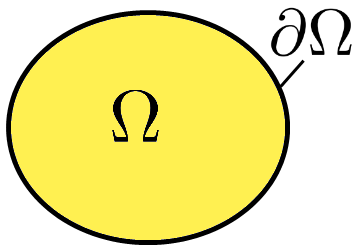
\includegraphics[width=3cm]{Content/Theory/Gebiet}&
	\end{tabular}
\end{minipage}
\begin{minipage}{4cm}	
	\begin{tabular}{ll}
		$\overset{\circ}{\Omega}$ & Innere Punkte\\
		$\partial\Omega$ & Rand\\
		$\overset{\_}{\Omega}$ & Gebiet $\Omega$ und Rand $\partial\Omega$\\
	\end{tabular}
\end{minipage}

Das Gebiet einer PDGL \textbf{muss} offen sein, nur dann ist die partielle
Ableitung überall definiert. Das Gebiet ist offen, wenn um jeden Punkt im Gebiet
$\Omega$ ein kleiner Ball gezeichnet werden kann, welches sich auch im Gebiet $\Omega$ befindet.\\

\begin{minipage}{4cm}
	Kein Gebiet:\\
	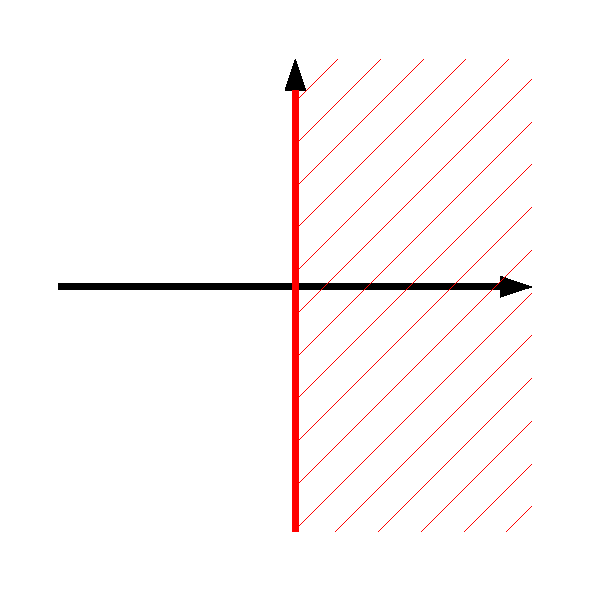
\includegraphics[width=4cm]{Content/Theory/gebiet_1.pdf}\\

\end{minipage}
\begin{minipage}{4cm}
  	Gebiet:\\
  	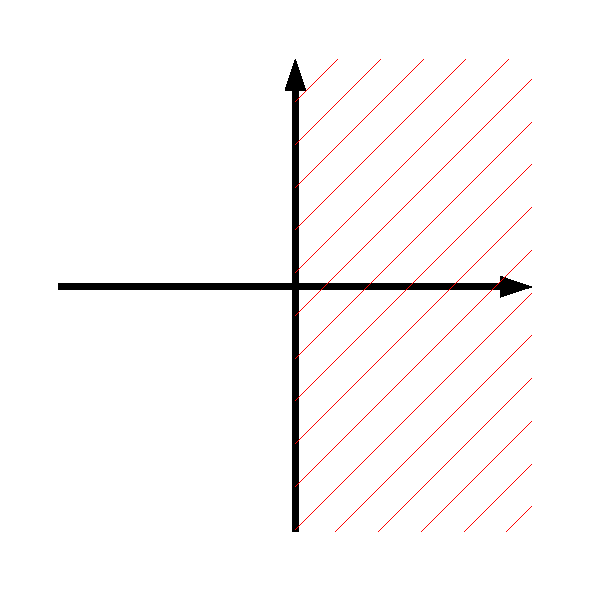
\includegraphics[width=4cm]{Content/Theory/gebiet_2.pdf}\\
\end{minipage}

\textbf{Lösung einer PDGL:}\\
\begin{tabular}{ll}
Gegeben:& Gebiet $\Omega$, PDGL,Randwerte $\partial\Omega$\\
Lösung:& Funktion $u$: $\overset{\_}{\Omega}\rightarrow \mathbb{R}$, PDGL in $\Omega$ und Randwerte auf $\partial\Omega$\\
\end{tabular} \\
'gut gestellt' wen die Angaben die Lösung eindeutig bestimmen

\subsubsection{Klassifikation einer PDGL}
\begin{tabular}{lll}
Ordnung:& \multicolumn{2}{l}{Höchste vorkommende partielle Ableitung}\\
Typ:& Linear: & Linear in $u, x_1,...,x_n, \frac{\partial u}{\partial x_1},\ldots,\frac{\partial u}{\partial x_n}$\\
& Quasilinear: &  Linear in $\frac{\partial u}{\partial x_1},\ldots,\frac{\partial u}{\partial x_n}$\\
& Nichtlineare: & Alles andere
\end{tabular}


\subsection{Method of Characteristics}

\textbf{Important:} Characteristics \textbf{cannot} be used as initial conditions, otherwise the characteristic becomes the solution (instead of obtaining a surface, you get a curve).\\
\textbf{Important:} The characteristic must pass through the boundary only once.\\
Useful for Quasilinear PDEs of 1st order. If separation is possible, this (simpler) method should be used.

Initial condition:
\[
    a(x,y,u)\cdot\partFrac{u}{x}+b(x,y,u)\cdot\partFrac{u}{y}-c(x,y,u)=0
\]
Characteristic:
\[
    \frac{d}{dt} \begin{bmatrix} x(t) \\ y(t) \\ u(t) \end{bmatrix}
    = \begin{bmatrix} a(x,y,u) \\ b(x,y,u) \\ c(x,y,u) \end{bmatrix}
\]


\begin{tabular}{ll}
Region:& $\Omega\{\ldots|x>0, \text{all }y\}$\qquad Boundary condition: $u(0,y_0)=g(y_0)$\\
Vector notation:& $\begin{bmatrix}
    a(x,y,u)\\ b(x,y,u)\\ c(x,y,u)
    \end{bmatrix}
\underset{\overrightarrow{n}\text{: Normal to surface}}{\underbrace{\begin{bmatrix}
\partFrac{u}{x} & \partFrac{u}{y} & -1
\end{bmatrix}}}=0 $ \\[1cm]
Tangents:& $\overrightarrow{t}_x=\begin{bmatrix}1\\0\\ \partFrac{u}{x}\end{bmatrix}\qquad
			\overrightarrow{t}_y=\begin{bmatrix}0\\1\\ \partFrac{u}{y}\end{bmatrix}\qquad \overrightarrow{n} \bullet \overrightarrow{t_x} = 0 \qquad \overrightarrow{n} \bullet \overrightarrow{t_y} = 0 \qquad \overrightarrow{t_x} \bullet \overrightarrow{t_y} = \overrightarrow{n}$\\[1cm]

Solution approach: & For each initial point $\begin{bmatrix} 0\\y_0\\g(y_0)\end{bmatrix}$ find a characteristic, then solve for $x$, $y$.
\end{tabular}

\paragraph{Boundary Conditions}
A solution function $u(x,y)$ must be covered by characteristics.
The solution is now determined by the boundary values.

\begin{minipage}{10cm}
    For the depicted region $\Omega$, different cases are possible:
    \begin{enumerate}
        \item Boundary values on the \emph{left} and \emph{right} are given. A region in the middle is undetermined.
        \item Boundary values on the \emph{upper} and \emph{lower} boundaries are given. A part of the region is over-determined.
        \item Boundary values on the \emph{left} and \emph{lower} boundaries are given. The function is uniquely determined (but not necessarily differentiable everywhere).
    \end{enumerate}
    The solution is not determinable for all boundary values. \newline
    If two characteristics meet $\rightarrow$ Singularity
\end{minipage}
\hspace{0.5cm}
\begin{minipage}{8cm}
    \centering
    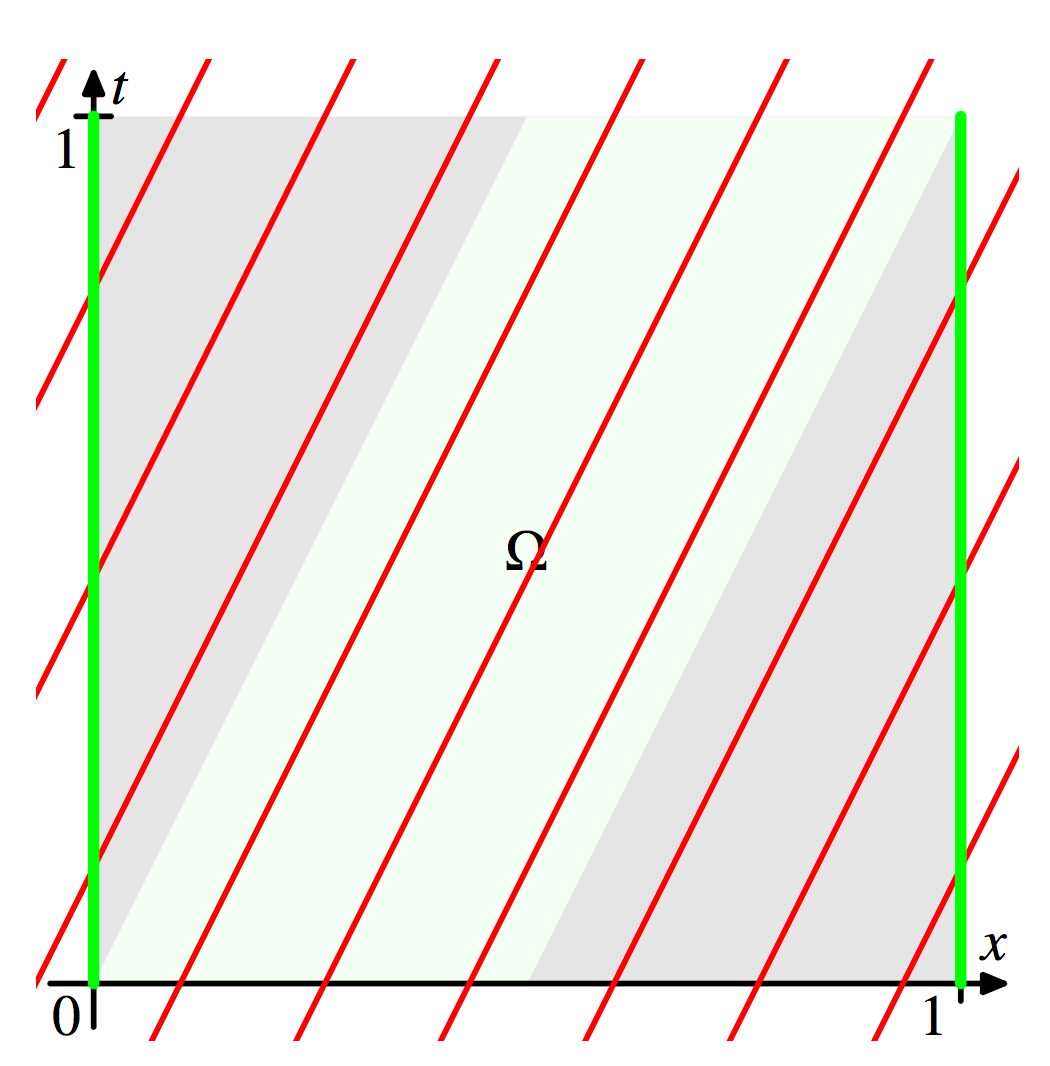
\includegraphics[width=6cm]{Content/01_theory/charakteristiken_randwerte.png}
\end{minipage}

\paragraph{Example:}~\\
\begin{enumerate}
	\item PDE with boundary conditions and domain: $\partFrac ux+2\partFrac uy=3$, \; $u(0,y)=g(y)=\sin(y) \Rightarrow u(0,y_0) = g(y_0) = \sin(y_0)$\\
	Terms in matrix form: $\begin{bmatrix}a\\b\\c\end{bmatrix}=\begin{bmatrix}1\\2\\3\end{bmatrix}$
	\item Calculate characteristics from PDE $\rightarrow$ ODE: 	$\frac {d}{dt}\begin{bmatrix}x(t)\\y(t)\\u(t)\end{bmatrix}=\begin{bmatrix}1\\2\\3\end{bmatrix}$
	\item Solve ODEs (for standard ODEs, see \ref{sec:dgls} on page \pageref{sec:dgls}.):
	$\begin{bmatrix}x\\y\\u\end{bmatrix}=\begin{bmatrix}1t+x_0\\2t+y_0\\3t+u_0\end{bmatrix}$
	\item Substitute initial conditions: $\begin{bmatrix}x\\y\\u\end{bmatrix}=\begin{bmatrix}1t+x_0\\2t+y_0\\3t+u_0\end{bmatrix}\Bigg|_{t=0}=
	\begin{bmatrix}x_0\\y_0\\u_0\end{bmatrix}=\begin{bmatrix}0\\y_0\\\sin(y_0)\end{bmatrix}$\\
	Solution of ODE is: $\begin{bmatrix}x\\y\\u\end{bmatrix}=\begin{bmatrix}1\\2\\3\end{bmatrix}\cdot t+ \begin{bmatrix}0\\y_0\\\sin(y_0)\end{bmatrix}$\\

	\item Eliminate all variables except $u,x,y$: $u=3x+\sin(y-2x)$
	\item Verification:
	Derive the result ($u=3x+\sin(y-2x)$) and substitute it into the original PDE $\partFrac ux+2\partFrac uy=3$ to check if it is satisfied.

\end{enumerate}


\subsection{Method Separation}
Choosing a suitable coordinate system is important.

\begin{enumerate}
\item \textbf{Approach} (Highest derivative decisive):
	\begin{itemize}
		\item For PDE 1st Order: $U(x,y)=X(x) + Y(y)$
		\item For PDE 2nd Order: $U(x,y)=X(x) \cdot Y(y)$
	\end{itemize}
\item \textbf{Substitution: } Substitute the approach into the PDE.
\item \textbf{Separation: } Each side of the PDE should only have one variable. The two resulting ordinary differential equations are coupled by a constant (fixing the variable). Choice of constant: If oscillation is expected, $-k^2$, otherwise $k$, unless you know better ;-).
\item \textbf{Solving the ODEs: } Obtain a family of solutions
\item \textbf{Constructing the General Solution: } (Linear combination of solutions), adhere to boundary conditions!
\end{enumerate}

\begin{minipage}{0.49\textwidth}
\textbf{Example 1: } PDE: $\frac1x\partFrac{u}{x}+\frac1y\partFrac{u}{y}=\frac{1}{y^2}$
\begin{enumerate}
	\item Approach:\\[0.4cm]
	$u(x,y)=X(x) + Y(y)$ (1st Order)
	\item Substitution:\\[0.4cm]
	$\partFrac{u}{x}=X'(x)$\qquad $\partFrac{u}{y}=Y'(y)$ \quad $\Rightarrow$ \quad $\frac{X'(x)}{x}+\frac{Y'(y)}{y}=\frac{1}{y^2}$
	\item Separation:\\[0.4cm]
	$\frac{X'(x)}{x}=k=\frac{1}{y^2}-\frac{Y'(y)}{y}$
	\item Solving ODEs:\\[0.4cm]
	$X'(x)=k\cdot x \quad\Rightarrow\quad X(x)=\frac12 kx^2+C_x$\\
	$Y'(y)=\frac1y-ky \quad\Rightarrow\quad Y(y)=\ln(y)-\frac12 ky^2+C_y$
	\item Linear Combination:\\[0.4cm]
	$u(x,y)=\frac12 kx^2 - \frac12 ky^2+ln(y)+C$
\end{enumerate}

\textbf{Example 2: } PDE: $x^2\partFrac{^2u}{x^2}+x\partFrac{u}{x}+y^2\partFrac{^2u}{y^2}+y\partFrac{u}{y}=0$\\
Boundary conditions: $\Omega=[1,2]\times[1,2]$ \qquad $u=0$ on $\partial\Omega$
\begin{enumerate}
	\item Approach:\\[0.4cm]
	$u(x,y)=X(x) \cdot Y(y)$ (2nd Order)
	\item Substitution:\\[0.4cm]
	$x^2X''(x)Y(y)+xX'(x)Y(y)+y^2X(x)Y''(y)+yX(x)Y'(y)=0$
	\item Separation: Division by $X(x)Y(y)$\\[0.4cm]
	$\frac{x^2X''(x)}{X(x)}+\frac{xX'(x)}{X(x)}+\frac{y^2Y''(y)}{Y(y)}+\frac{yY'(y)}{Y(y)}=0\quad\Rightarrow\quad \frac{x^2X''(x)}{X(x)}+\frac{xX'(x)}{X(x)}=k=-\frac{y^2Y''(y)}{Y(y)}-\frac{yY'(y)}{Y(y)}$
	\item Solving ODEs:\\[0.4cm]
	$\frac{x^2X''(x)}{X(x)}+\frac{xX'(x)}{X(x)}=k\quad\Rightarrow\quad x^2X''(x)+xX'(x)-kX(x)=0$\qquad with $X(1)=X(2)=0$\\
	$\frac{y^2Y''(y)}{Y(y)}-\frac{yY'(y)}{Y(y)}=-k\quad\Rightarrow\quad y^2Y''(y)+yY'(y)+kY(y)=0$\qquad with $Y(1)=Y(2)=0$\\[0.4cm]
	Solution of ODEs not done here.
\end{enumerate}
\end{minipage}
\hfill
\begin{minipage}{0.49\textwidth}
\textbf{Example 3: }PDE: $\partFrac{^2u}{t^2}=\partFrac{^2u}{x^2}$ \quad $u(t=0,x)=0$\\
Boundary conditions: $x=[0,\pi]$ \\
\qquad\qquad $\partFrac{u}{t}(t=0,x)=\sin^3(x)=\frac34\sin(x)-\frac14\sin(3x)$
\begin{enumerate}
	\item Approach:\\[0.4cm]
	$u(t,x)=T(t) \cdot X(x) $ (2nd Order)
	\item Substitution:\\[0.4cm]
	$T''(t)\cdot X(x) = X''(x)\cdot T(t)$
	\item Separation:\\[0.4cm]
	$\frac{X''(x)}{X(x)}= -\mu^2=\frac{T''(t)}{T(t)}$
	\item Solving ODEs:\\[0.4cm]
		$X(x)=\sin(\mu x) \qquad T(t)=\sin(\mu t)$\\
		$X(x)=\cos(\mu x) \qquad T(t)=\cos(\mu t)$
	\item Linear Combination:\\[0.4cm]
		The boundary conditions $x=0$ and $x=\pi$ can only be satisfied with $\sin(\mu x) $ and positive, integer $\mu$. $cos(nx)$ terms are eliminated.\\[0.4cm]
		$u(t,x)=\sum\limits_{n=1}^{\infty}{a_n\sin(nx)\sin(nt)} + \sum\limits_{n=1}^{\infty}{b_n\sin(nx)\cos(nt)}$\\[0.4cm]
		The coefficients $a_n$ and $b_n$ must be determined using the initial conditions at time $t=0$:\\[0.4cm]
		$u(0,x)=\sum\limits_{n=1}^{\infty}{b_n\sin(nx)}=0 \quad\Rightarrow\quad b_n=0$\\[0.2cm]
		$\partFrac{u}{t}(\pi,x)=\sum\limits_{n=1}^{\infty}{a_nn\sin(nx)}=\sin^3(x)=\frac34\sin(x)-\frac14\sin(3x) \quad\Rightarrow\quad a_1=\frac34 \quad a_3=-\frac{1}{12}\quad a_k=0$ for $k\neq 1,3$\\[0.4cm]
		$u(t,x)=\frac34\sin(x)\sin(t)-\frac1{12}\sin(3x)\sin(3t)$
\end{enumerate}
\end{minipage}


\subsection{Hamilton-Jacobi Theorie}
Die Hamilton-Jacobi Theorie geht von einer Gesamtenergie $H(x_i,p_i)$ in Abhängigkeit von Ort
und Impuls aus.
Dazu muss eine Funktion $S(x_i,t)$ gefunden werden, für welche
\begin{align*}
    \frac{\partial S}{\partial t} = H\left(x_i,p_i\right) = H\left(x_i,\frac{\partial S}{\partial x_i}\right)
    && \text{mit} \quad
    p_i = \frac{\partial S}{\partial x_i}
\end{align*}
Diese kann meist durch Integration gelöst werden.
Dabei werden die Integrationskonstanten $P_i$ eingeführt.
Die \emph{Bahnparameter} $Q_i$ sind
\[
    Q_i = \frac{\partial S}{\partial P_i}
\]
und die Bahnkurve hat die Form
\[
    x_i(t,Q_i,P_i)
\]

\begin{landscape}

\begin{minipage}{7cm}
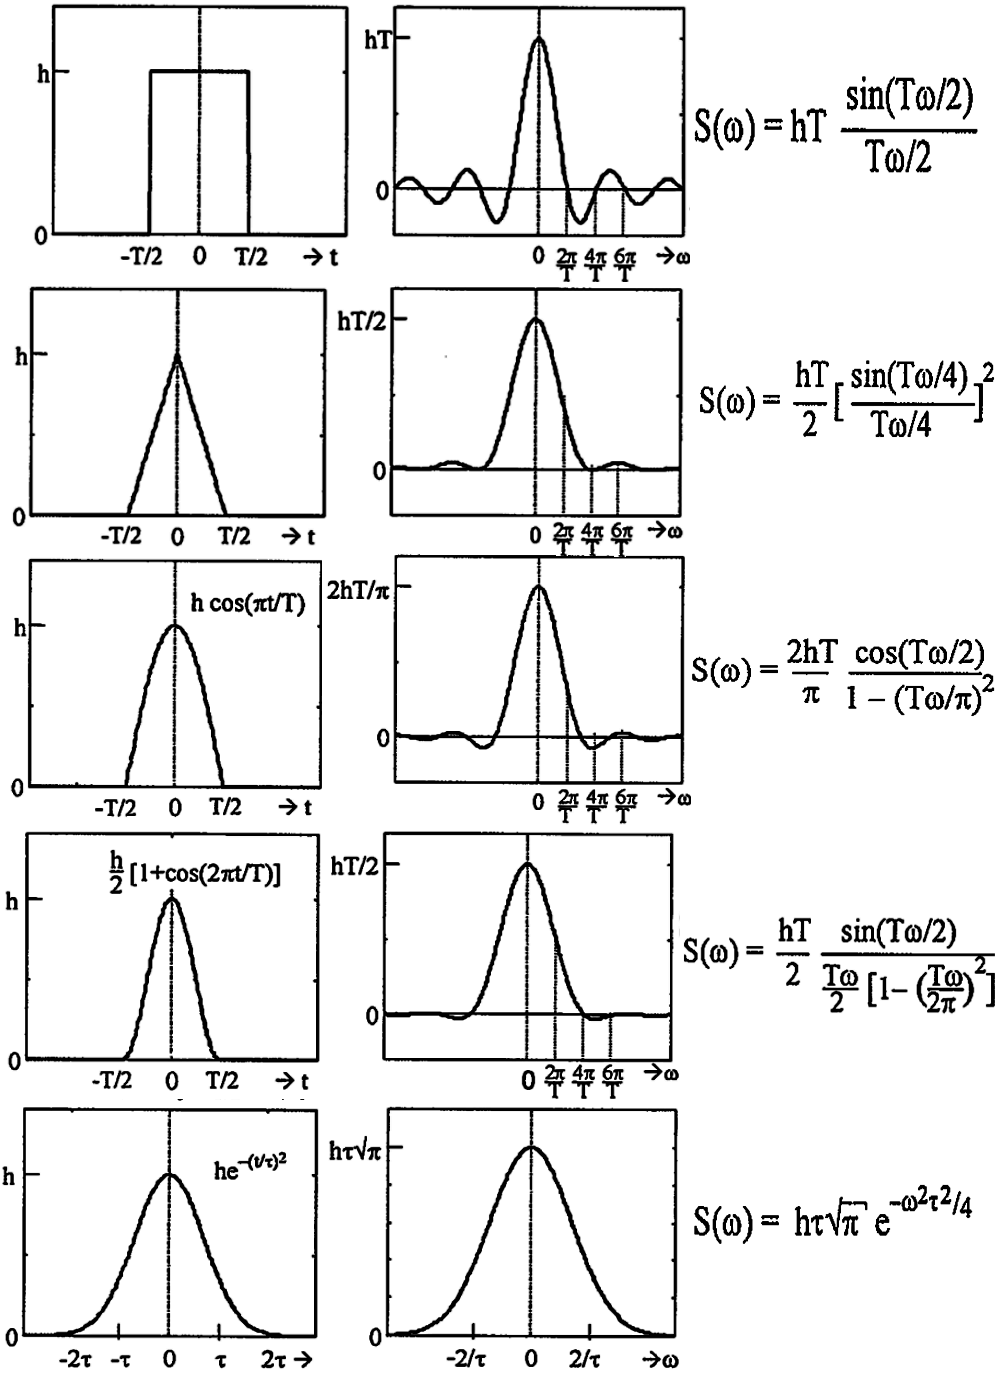
\includegraphics[width=\textwidth,trim= 0cm 0cm 0cm 0cm]{bilder/Transformationen/Fourier-Trafo.png}

\end{minipage}
\begin{minipage}{8.25cm}
	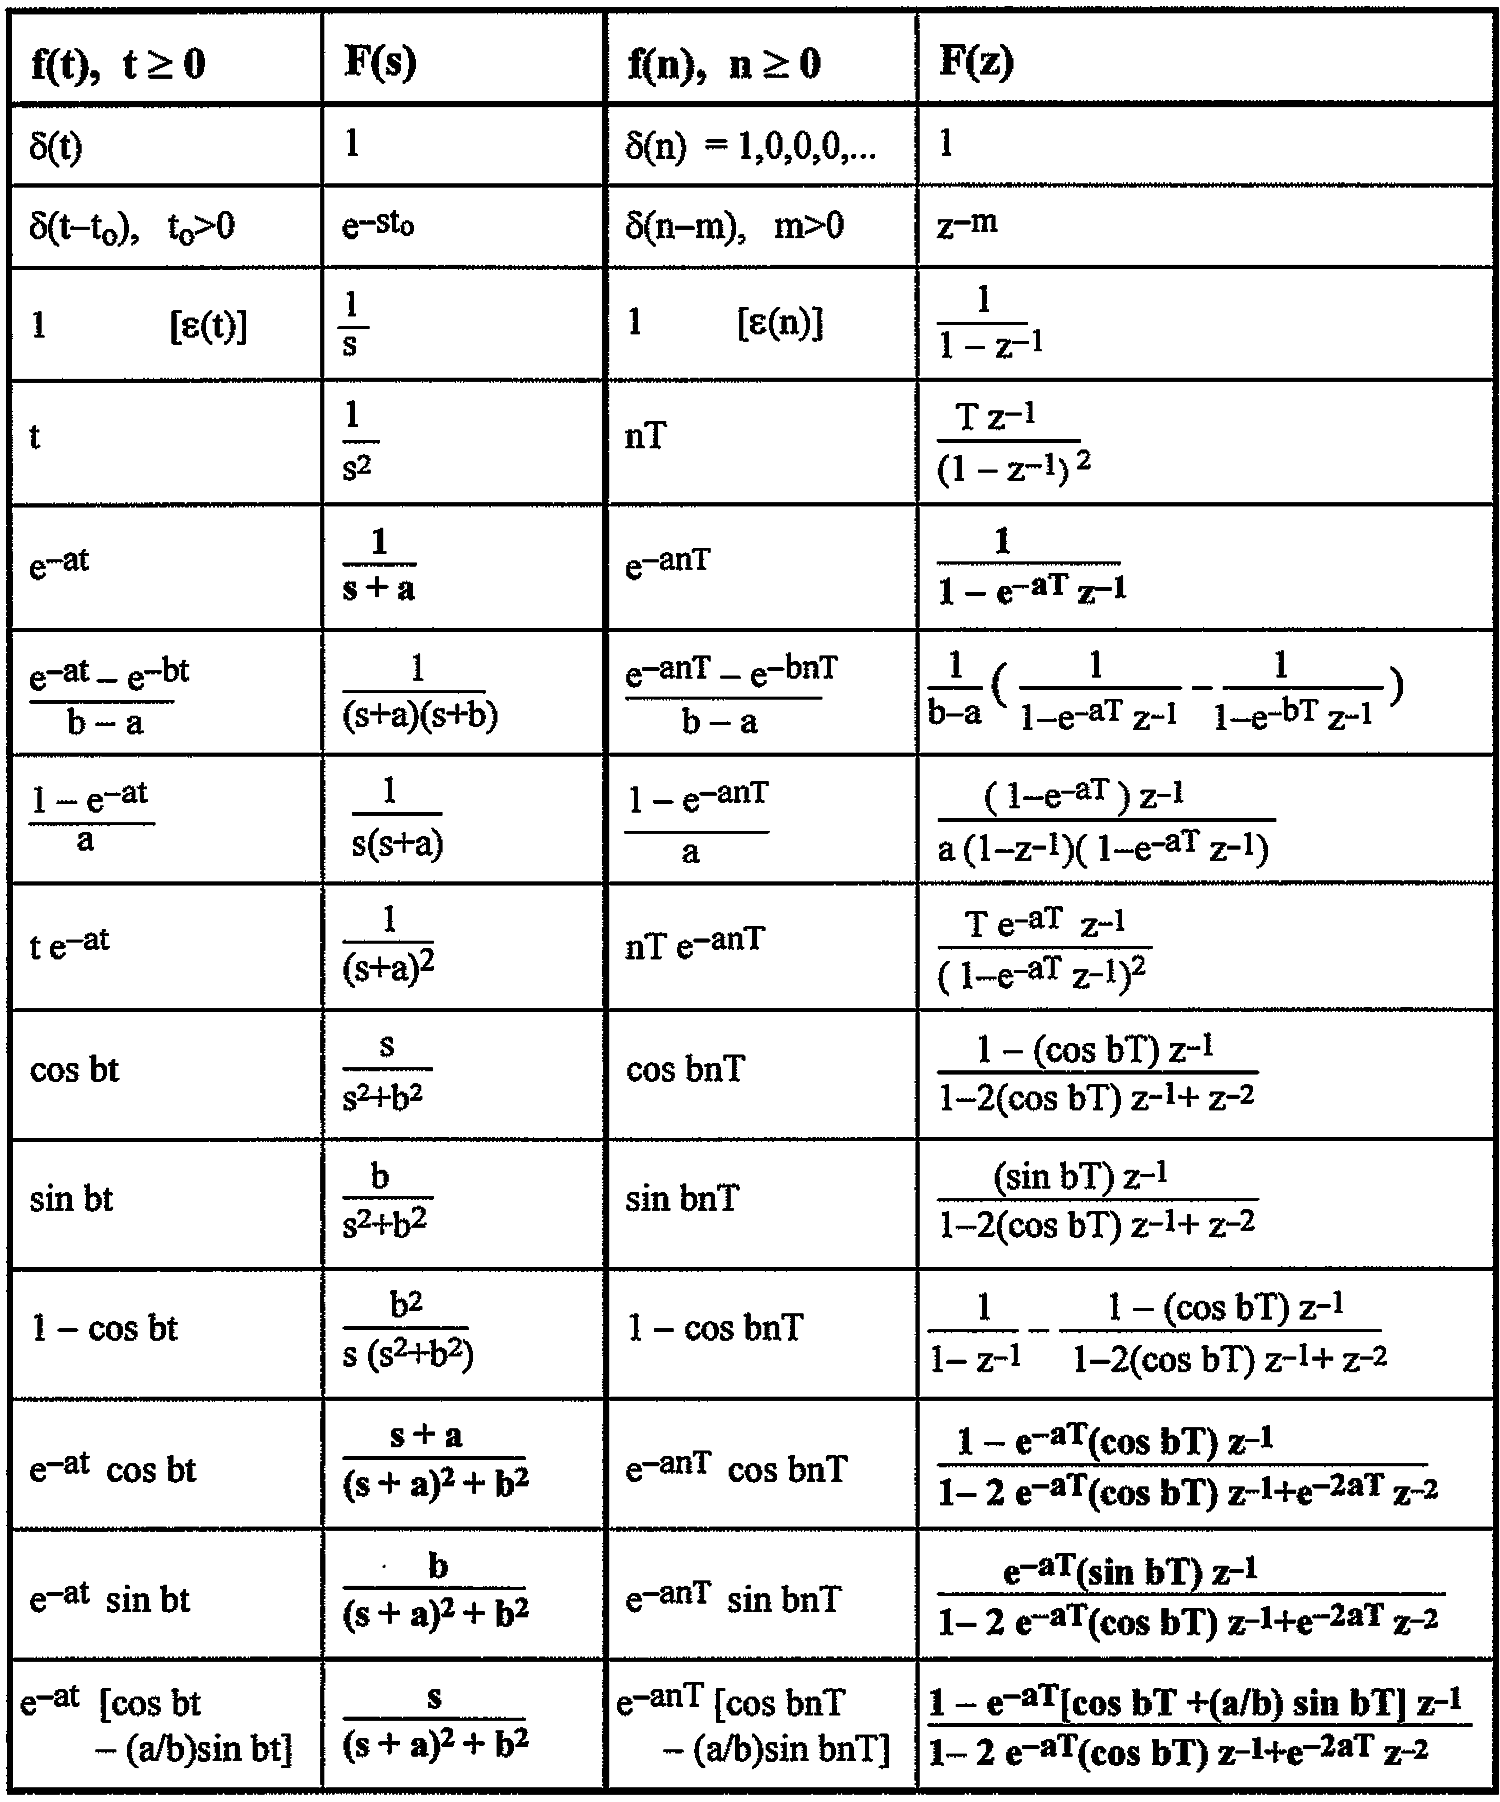
\includegraphics[width=\textwidth,trim= 0cm 0.3cm 0cm 0.45cm]{bilder/Transformationen/Z-Lexikon.png}
	\end{minipage}
	\begin{minipage}{10cm}
	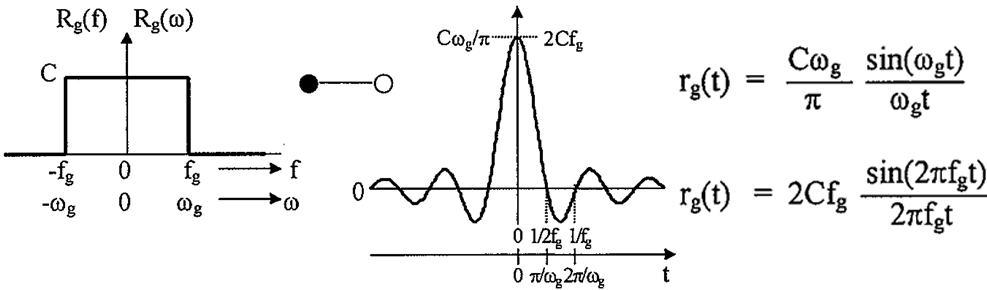
\includegraphics[width=\textwidth,trim= 0cm 0cm 0cm 0cm]{bilder/Transformationen/Rechteck-Sinc.png}
	\textbf{Matrizeninversion}\\
	$A^{-1} = \begin{pmatrix}
	a & b \\ c & d \\
	\end{pmatrix}^{-1} =
	\frac{1}{\det(A)} \begin{pmatrix}
	d & -b \\ -c & a \\
	\end{pmatrix}  =
	\frac{1}{ad-bc} \begin{pmatrix}
	d & -b \\ -c & a \\
	\end{pmatrix}\quad$\\
	$A^{-1} = \begin{pmatrix}
	a & b & c\\ d & e & f \\ g & h & i \\
	\end{pmatrix}^{-1} =
	\frac{1}{\det(A)} \begin{pmatrix}
	ei - fh & ch - bi & bf - ce \\
	fg - di & ai - cg & cd - af \\
	dh - eg & bg - ah & ae - bd
	\end{pmatrix}$\\
	\begin{minipage}{4cm}
		\textbf{Trigonometrie} \\
		$e^{j\varphi}=\cos(\varphi)+ j \cdot \sin(\varphi) $
		$e^{-j\varphi}=\cos(\varphi)- j \cdot \sin(\varphi) $
		$\cos(x) = \frac{e^{jx} + e^{-jx}}{2}$\\
		$\sin(x) = \frac{e^{jx} - e^{-jx}}{2j}$\\
		$\cos^2(x) = \frac12 + \frac{\cos(2x)}{2}$\\
		$\sin^2(x) = \frac12 - \frac{\cos(2x)}{2}$\\
		$\sin(2x)=2\sin(x)\cdot\cos(x)$\\
		$\sin^2(x)+\cos^2(x)=1$
	\end{minipage}
	\begin{minipage}{5cm}
		\textbf{Determinanten} \\
		\footnotesize
		$\det \begin{pmatrix} a & b \\ c & d\\ \end{pmatrix} =
		a d - b c \quad$\\
		$\det \begin{pmatrix} 
		a & b & c \\
		d & e & f \\
		g & h & i  \end{pmatrix}
		= a e i + b f g + c g h \\
		\text{\hspace{2.5cm}} -c e g - f h a - i b d$		\normalsize
	\end{minipage}
\end{minipage}

%\section{Fourier Transformation}
\begin{minipage}{0.85\linewidth}
%\subsubsection{Eigenschaften von Fourier- und Z-Transformation}
\footnotesize 
\renewcommand{\arraystretch}{1.1}
\begin{tabular}{|p{4.3cm}||p{1.8cm}|p{1.8cm}||p{2.2cm}|p{2.4cm}||p{1.9cm}|p{2.6cm}|}
\hline
\textbf{Bezeichnung}
  & \multicolumn{2}{|c||}{\textbf{Zeitbereich}}
  & \multicolumn{2}{|c||}{\textbf{Kontinuierlicher Frequenzbereich}}
  & \multicolumn{2}{|c|}{\textbf{Diskreter Frequenzbereich}} \\
  & \textbf{kontinuierlich}
  & \textbf{diskret}
  & \textbf{Fourier-Integral} 
  & \textbf{Laplace}
  & \textbf{Diskrete FT} 
  & \textbf{Z-Transformation} \\
\hline
\hline
  Linearität 
  & $\alpha\cdot f(t) + \beta\cdot g(t)$
  & $\alpha\cdot f(n) + \beta\cdot g(n)$
  & $\alpha\cdot F(\omega) + \beta\cdot G(\omega)$
  & $\alpha\cdot F(s) + \beta\cdot G(s)$
  & $\alpha\cdot F(n) + \beta\cdot G(n)$
  & $\alpha\cdot F(z) + \beta\cdot G(z)$\\
\hline
  "Ahnlichkeit / Zeitskalierung bzw. Spiegelung an Y-Achse
  &	$f(\alpha t)$ 
  & $f(-n)$
  & $\frac{1}{|\alpha|}F \left (\frac{\omega}{\alpha} \right)$
  & $\frac{1}{\alpha}F \left (\frac{s}{\alpha} \right )$ 
  & $F(-n)$
  & $F(z^{-1})$\\
%\hline
  %D�mpfung
  %& -
  %& $e^{dn} f(n)$
  %& -
  %& - 
  %& -
  %& $F(z e^{d})$ \\
\hline
  Verschiebung im Zeitbereich 
  & $f(t\pm t_0)$ 
  & $f(n \pm n_0)$
  & $e^{\pm j\omega t_0} F(\omega)$
  & $F(s)e^{\pm t_0 s}$ 
  & $e^{\pm j\frac{n}{N}2 \pi n_0} F(n)$
  & $z^{\pm n_0} F(z)$\\
\hline
  Verschiebung im Frequenzbereich 
  & $f(t)e^{\mp\alpha t}$ 
  & $f(n) e^{\mp j \frac{n}{N} 2 \pi n_0}$
  & $F(\omega\pm \alpha)$
  & $F(s\pm\alpha)$ 
  & $F(n \pm n_0)$
  & $F(z \pm n_0)$\\
\hline
  Faltung im Zeitbereich 
  &	$f(t) \ast g(t)$
  & $f(n) \ast g(n)$
  & $F(\omega) \cdot G(\omega)$
  & $F(s) \cdot G(s)$
  & $F(n) \cdot G(n)$ 
  & $F(z) \cdot G(z)$ \\
\hline
  Faltung im Frequenzbereich 
  &	$f(t) \cdot g(t)$
  & $f(n) \cdot g(n)$
  & $\frac{1}{2\pi} F(\omega) \ast G(\omega)$
  & $\frac{1}{2\pi} F(s) \ast G(s)$ 
  & $\frac{1}{N} F(n) \ast G(n)$
  & $\frac{1}{N} F(z) \ast G(z)$\\
\hline
  Ableitungen im Zeitbereich bzw. Differenzenbildung 
  & $\frac{\partial^n f(t)}{\partial t^n}$ 
  & $\Delta^k f(n)$
  & $(j\omega)^n F(\omega)$
  & $s^nF(s)-s^{n-1}f(0+)-s^{n-2}\frac{\partial f(0+)}{\partial t}-\ldots
 			-s^0\frac{\partial^{n-1} f(0+)}{\partial t^{n-1}}$
  & 
  & $(1-z^{-1})^k F(z)$ \\
\hline
  Ableitung im Frequenzbereich
  & $(-t)^k\cdot f(t)$ 
  & $n f(n)$ 
  & $j^k \frac{-\partial^k F(\omega)}{\partial \omega^k}$
  & $\frac{\partial^k F(s)}{\partial s^k}$
  & 
  & $-z \frac{\partial F(z)}{\partial z}$ \\
\hline 			
  Integration bzw. Summierung
  & $\int\limits_{-\infty}^t f(\tau)d\tau$ 
  & $\sum\limits_{n=0}^{k} f(n)$
  & $\frac{F(\omega)}{j\omega}+F(0)\pi\delta(\omega)$
  & $\frac{F(s)}{s}$
  & 
  & $\frac{1}{1-z^{-1}} F(z)$ \\
\hline
  Anfangswert 
  & $\lim\limits_{t\rightarrow 0} f(t)$ 
  & $f(0)$
  & 
  & $\lim\limits_{s\rightarrow \infty} sF(s)$ 
  & 
  & $\lim\limits_{z \rightarrow \infty} F(z)$ \\
\hline
  Endwert
  &	$\lim\limits_{t\rightarrow \infty} f(t)$
  & $\lim\limits_{n\rightarrow \infty} f(n)$
  & 
  & $\lim\limits_{s\rightarrow 0} sF(s)$
  & 
  & $\lim\limits_{z \rightarrow 1} (1-z^{-1}) F(z))$\\
%\hline
  %Stabilit�t
  %& -
  %& -
  %& -
  %& Pole in LHE
  %& 
  %& Pole innerhalb Einheitskreis \\
%\hline
  %Kausalit�t
  %& -
  %& -
  %& A- \& Kausal
  %& Nur Kausal
  %& 
  %& $\lim\limits_{z \rightarrow \infty} z^{-1} F(z) = 0$ \\
\hline
\hline
  Spezial
  & \multicolumn{3}{l||}{
      Bessel-Theorem \qquad
      $\int\limits_{-\infty}^{\infty}f(t)g^{\ast}(t)dt =
         \frac{1}{2\pi}
         \int\limits_{-\infty}^{\infty}F(\omega)G^{\ast}(\omega)d\omega$}
  & \multicolumn{3}{|l|}{
      Parseval-Theorem \qquad
      $W = \int\limits_{-\infty}^{\infty}|f(t)|^2 dt = \frac{1}{2\pi}
      \int\limits_{-\infty}^{\infty}|F(\omega)|^2 d\omega$
    }\\
\hline

\end{tabular}
\end{minipage}
\begin{minipage}{0.2\linewidth}
\textbf{Quadratische Gleichung:}\\
$a\cdot x^2+b\cdot x +c=0$\\

$x_{1,2}=\frac{-b\pm \sqrt{b^2-4ac}}{2a}$\\

\textbf{Fouriertransformation:}\\

$\delta(t)\FT 1$\\
$1\FT 2\pi \delta(\omega)$\\
$\sigma(t)\FT \frac{1}{j\omega}+\pi\delta(\omega)$\\
$\text{sgn}(t)\FT \frac{2}{j\omega}$\\
$e^{\pm j \omega_0 t} \FT 2\pi \delta(\omega \mp \omega_0)$\\
$\sin(\omega_0t)\FT j\pi(\delta(\omega +\omega_0)-\newline\text{\hspace{2.7cm}}\delta(\omega -\omega_0))$\\
$\cos(\omega_0t)\FT \pi(\delta(\omega +\omega_0)+\newline\text{\hspace{2.6cm}}\delta(\omega -\omega_0))$\\
\end{minipage}


%% We don't need this and it does not fit onto the page. The trigonometric relationships are already on this page under ''Trigonometrie'', and the z-transforms are in the z-transform table. 
%% In my opinion the z-transform table should also be updated, because you can barely read it when it's included as a picture and scaled. 
 
% \begin{minipage}{\linewidth}
% \vspace*{-1cm}
% $e^{j\omega}=\cos(\omega) + j \cdot \sin(\omega)$
% \quad
% $\sin(\omega)=\dfrac{e^{j\omega} - e^{-j\omega}}{2j}$
% \quad
% $\cos(\omega)=\dfrac{e^{j\omega} + e^{-j\omega}}{2}$
% \quad
% $1\pm e^{-j\omega T}= (e^{j\frac{\omega}{2} T}\pm e^{-j\frac{\omega}{2} T})\cdot e^{-j\frac{\omega}{2} T}$
% \quad
% $a^n \FT \frac{1}{1-az^-1}$
% \quad
% $a^{|n|} \FT \frac{1-a^2}{(1-az^-1)(1-az)}$
% \quad
% \vspace*{-2cm}
% \end{minipage}


\end{landscape}

\subsection{PDE 2nd Order}
Linear partial differential equations of second order have the form:
$\boxed{\sum\limits_{i,j=1}^{n}{a_{ij}\partial_i\partial_j u}+\sum\limits_{i=1}^{n}{b_i\partial_i u}+cu=f}$

\subsubsection{Classification}
Classification only for PDEs of second order!

\begin{minipage}{9cm}
  Eigenvalue calculation: (e.g., for $ \partial^2_xu+2\partial_x\partial_yu+\partial^2_yu=0 $)
  \begin{enumerate}
    \item Form a symmetric matrix and subtract $\lambda$ on the diagonal. For example: $A = \begin{pmatrix}
      \partial_x^2 & \partial_x \partial_y \\
      \partial_y \partial_x  & \partial_y^2
    \end{pmatrix}$\\
    In diagonal matrices, the eigenvalues correspond to the diagonal entries.
    \item Set determinant equal to 0: $\det(\mathbf{A}-\lambda \mathbf{I}) = 0\quad\Rightarrow\quad \lambda_i$
    \item Solve the equation
  \end{enumerate}
\end{minipage}
\hfill
\begin{minipage}{9cm}
  Alternatively (if, for example, a very complicated PDE needs to be classified), the signs of the eigenvalues can also be determined via trace and determinant:
  \begin{enumerate}
    \item See left (Eigenvalue calculation): Form matrix $A$
    \item Calculate determinant and try to read from the table:
     $\det A = a_{11}a_{22} - a_{12}a_{21} = \lambda_1 \lambda_2$
    \item Calculate trace and try to read from the table:
      $\tr(A) = a_{11} + a_{22} = \lambda_1 + \lambda_2$
  \end{enumerate}
\end{minipage}

\begin{center}
\begin{tabular}{|l||l|l|l|l|l|}
\hline
\multirow{2}{*}{Class}&\multicolumn{3}{|c|}{Number of Eigenvalues} & det(A)&\multirow{2}{*}{Example}\\
& Positive & Negative & Zero(=0) & for n=2 &\\
\hline
Hyperbolic& n-1 & 1 & 0 & det < 0 & Wave Equation: $\frac{\partial^2 u}{\partial t^2} = \Delta u$ \\
\hline
Parabolic& n-1 & 0 & 1 & det = 0 & Heat Equation: $\frac{\partial u}{\partial t} = \Delta u$  \\
\hline
Elliptic&	n & 0 & 0 & det > 0 & Potential: $\Delta u = f$ \\
\hline
Ultrahyperbolic & >1 & >1 & 0 & - & -\\
\hline
\end{tabular}
\end{center}


\subsection{Elliptische PDGL}
$\Delta u=f\qquad \omega=\{(x,y)|y\geq 0\},\quad u(x,y)=ay$

\textbf{Satz:} Wenn $\Omega$ beschränkt und zusammenhängend, dann ist die Lösung u immer eindeutig.\\

\textbf{Beweis:} Annahme: $u=u_1-u_2$\\
Einsetzen: $\Delta u_1 - \Delta u_2=f-f=0$\\
$\left.(u_1-u_2)\right|_{\partial \omega}=g-g=0$\\
$\Delta u=0 \qquad \left.u\right|_{\partial\Omega}=0$\\
Falls $u=0$ eine Lösung, dann gibt es nur eine Lösung.

\subsubsection{Maximumprinzip} 

Wenn gilt $\Delta u=0$, so ist $u$ \emph{harmonisch}, und dann befinden 
sich die Extrema (Maxima und Minima der Funktion) auf dem Rand $\partial\Omega$.

\subsubsection{Beispiel (Übungslösungen)}
Eine elliptische PDGL wie $\Delta u = c$ hat mit der vorgegebenen
Dirichlet-Randwerten nur eine Lösung. Zur Erinnerung: Der Grund war das
Maximum-Prinzip. Gäbe es nämlich eine zweite Lösung $\bar v(r,\phi)$ mit
gleichen Randwerten, wäre $v - \bar v$ eine Lösung der Gleichung $\Delta (v -
\bar v) = 0$ also harmonische Funktion. Die Randwerte von $v - \bar v$ sind 0. Da eine
harmonische Funktion das Maximum auf dem Rand annimmt ist $v - \bar v = 0$ die
Lösung ist also eindeutig.

\newpage
\subsubsection{Greensche Funktion} 

Eine elliptische PDGL wird mittels Inversion von $\Delta$ gelöst. Dieser Umkehr geschieht mittels Greenscher Funktion, welche die Umkehrfunktion $\Delta$ ist\qquad $\Delta$: Laplace-Operator.

$u(x)=\int\limits_\Omega{\sigma(x,\xi)f(\xi)d\xi}+\int\limits_\Omega{h(x,\xi)f(\xi)d\xi}\qquad \sigma(x,\xi)=
\begin{cases}
	\frac 12|x-\xi| & n=1\\ 
	\frac 1{2\pi}\log|x-\xi| & n=2\\
	-\frac 1{4\pi}\frac{1}{|x-\xi|} & n=3\\
	\frac {1}{(2-n)\mu(S^{n-1})}|x-\xi|^{2-n} & n\geq 3\\
\end{cases}$\\


Greensche Funktion: $G(x,\xi)=\sigma(x,\xi)+h(x,\xi)$

Satz: Ist $\Omega$ ein Gebiet, auf dem das Dirichlet Problem eindeutig lösbar ist, dann gibt es eine Funktion $G(x,\xi)$, welche als Funktion von x die Gleichung

$\Delta G(x,\xi)=\delta(x-\xi)$

löst mit homogenen Randbedingungen.
Lösung: $u(x)=\int\limits_{\Omega}^{}{G(x,\xi)f(\xi)d\xi}+\int\limits_{\partial\Omega}g(\xi)\cdot\grad{\xi}G(x,\xi)d\eta\qquad \eta:\text{ Normale von }\partial G$

\subsubsection{Mittelwerteigenschaft harmonischer Funktionen}

$\Delta h=0$\qquad Mittelwerteigenschaft:\qquad $h(x)=
\begin{cases}
	\frac{h(x+\delta)+h(x-\delta)}{2}& n=1 \\ 
	\frac 1{2\pi r} \int\limits_{S_r^1}{h(x+\xi)d\xi} & n=2\\
	\frac 1{4\pi r^2} \int\limits_{S_r^2}{h(x+\xi)d\xi} & n=3\\
\end{cases}$
%\subsection{Parabolische PDGL}
\todo{Beschreibung}
\subsection{Hyperbolische PDGL}
\begin{minipage}{14cm}
	PDGL: $\partFrac{^2u}{t^2}-a^2\partFrac{^2 u}{x^2}=0\qquad \Omega=\left\{(x,t)|t>0\right\}\qquad u_0=u(x_0,0)$\\
	
	Trick: $(\partial_t +a\partial_x)(\partial_t-a\partial_x)u=(\partial_t^2-a^2\partial_x^2)u=0$\qquad(für konstante Geschwindigkeit $a$)\\
	
	Zwei mögliche Lösungen: $\underset{\text{\cfbox{red}{Nach rechts laufende Welle}}}{\underbrace{(\partial_t +a\partial_x)u=0}}\qquad \underset{\text{\cfbox{black}{Nach links laufende Welle}}}{\underbrace{(\partial_t-a\partial_x)u=0}}$\\
	
	Lösung mittels Charakteristiken: $\partFrac{}{s}
	\begin{Bmatrix}
		x(s)\\
		t(s)\\
		u(s)
	\end{Bmatrix}=
	\begin{Bmatrix}
		\pm a\\
		1\\
		0
	\end{Bmatrix}
	\begin{array}{ll}
		\Rightarrow&x=\pm as +x_0\\
		\Rightarrow&t= s +t_0=s\qquad (t_0=0)\\
		\Rightarrow&u=u_0\\
	\end{array}
	$\\
	
	$x=\pm at+x_0\quad\Rightarrow\quad x_0=x\mp at\quad\Rightarrow\quad u(x,t)=u_0(x\mp at)$\\
	
	Allgemeine Lösung aus Linearkombination: $\boxed{u(x,t)=u_+(x+at)+u_-(x-at)}$\\
	
	$\Rightarrow$ Es werden \textbf{zwei} Anfangsbedingungen benötigt um $u_+$ \textbf{und} $u_-$ zu bestimmen.\\
	
	z.B.: $u(x,0)=u_0(x)\qquad \partFrac{u}{t}(x,0)=g_0(x)$
	\end{minipage}
	\hfill
	\begin{minipage}{5cm}
	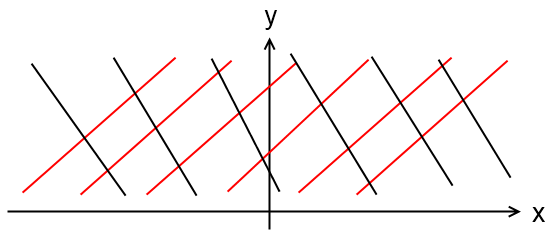
\includegraphics[width=5cm]{Content/01_theory/linksRechts}
	\end{minipage}
\subsubsection{Streifen/Charakteristiken}
	PDGL: $a\partial_x^2u+2b\partial_x\partial_yu+c\partial_y^2u+d\partial_xu+e\partial_yu+fu=g$ Symbolmatrix: $ 
		\begin{bmatrix}
			a & b\\
			b & c
		\end{bmatrix}$
	
	Entlang der Kurve $t\mapsto(x(t),y(t))$ sind die Anfangswerte / partiellen Ableitungen
	$
	\left.
	\begin{aligned}
	u(x(t),y(t))&=u(t)\\
	\partial_xu(x(t),y(t))&=p(t)\\
	\partial_yu(x(t),y(t))&=q(t)
	\end{aligned}
	\qquad
	\right\}
	\label{charanfangs}
	$
	
	Charakteristiken erfüllen DGL:
    \[
        a\dot y(t)^2-2b\dot x(t)\dot y(t)+c\dot x(t)^2=0
    \]
	
	Charakteristischer Streifen erfüllt zusätzlich: $a\dot p(t)\dot y(t)-h\dot x(t)\dot y(t)+c\dot x(t)\dot q(t)=0$



\newpage

\section{Numerik}
\subsection{Diskretisierung}
\subsubsection{1.Ableitung}

$$g'(x)\approx \frac{g(x+\Delta x)-g(x)}{\Delta x} \qquad\qquad \text{oder}
\qquad\qquad \boxed{g'(x)\approx \frac{g(x+\Delta x)-g(x-\Delta x)}{2\Delta
x}}\qquad \text{(Zentrale Differenz: Bessere Qualität)}$$
\subsubsection{2.Ableitung}
$\boxed{g''(x)\approx \frac{g(x-\Delta x)-2 g(x) + g(x+ \Delta x)}{\Delta x^2}}$ ist für zweite (bessere Qualität) Version die Gleiche

\subsection{FDM}
\textbf{TIPP:} Bei Anfangsbedingungen ungleich Null das Gleichungssystem selber von Hand herleiten, reduziert die Chance auf Fehler.
\subsubsection{Grundgleichung: $-u''(x)=f(x)$}
$ A^{(n)} \tilde{u}^{(n)} =f^{(n)}   $\\
$A^{(n)}= \frac{1}{\Delta x^2} \tridiag_{n-1} (-1,2,-1) = \frac{1}{\Delta x^2}
  \begin{bmatrix}
             2& -1 & 0 & \ldots \\
             -1& 2 & -1 & \ldots \\
              0& -1 & 2 & \ldots \\
              0& 0 & -1 & \ldots \\
             \ldots
           \end{bmatrix}$\qquad (eine $(n-1)\times(n-1)$-Matrize)\\
Randwert: $u(0)= a \qquad u(n)=b $ \qquad
$A^{(n)}\tilde{u}^{(n)} =\begin{bmatrix}
             f(x_1^{(n)}) + \dfrac{a}{\Delta x^2} \\
             f(x_2^{(n)}) \\
             \vdots  \\
             f(x_{(n-1)}^{(n)}) + \dfrac{b}{\Delta x^2}
           \end{bmatrix} $\\
\subsubsection{Grundgleichung: $T''(x) -  h T(x) = T_A$}
$-T'' + h T(x) = h T_A$\\
$A^{(n)}= \frac{1}{\Delta x^2} \tridiag_{n-1}
(-1,2+h\Delta x^2,-1) = \frac{1}{\Delta x^2}
  \begin{bmatrix}
             2+h\Delta x^2& -1 & 0 & \ldots \\
             -1& 2+h\Delta x^2 & -1 & \ldots \\
              0& -1 & 2+h\Delta x^2 & \ldots \\
              0& 0 & -1 & \ldots \\
             \ldots
           \end{bmatrix} $\\

\subsubsection{Beispiel Hausübung 7}
Gegeben: $ u''(x)=4(u(x)-x) $ mit den Randwerten $ u(0)=0 $  und $ u(1)=2 $ mit $\Delta x=1/3$.
\\
Gesucht: $ \tilde{u}(\frac{1}{3}) $ und $ \tilde{u}(\frac{2}{3}) $
\\
Lösen: Die Ableitung von $ u'' $ einsetzen, siehe oben, ergibt die allgemeine Gleichung von $ \frac{u(x-\Delta x)-2 u(x) + u(x+ \Delta x)}{\Delta x^2} =4 (u(x)-x) $, für die Punkte P1 und P2 ergibt das.
\\
P1: $ \frac{0-2 \tilde{u}(\frac{1}{3}) + \tilde{u}(\frac{2}{3})}{(\frac{1}{3})^2} =4(\tilde{u}(\frac{1}{3})-\frac{1}{3}) $
\qquad \qquad
P2: $ \frac{\tilde{u}(\frac{1}{3})-2 \tilde{u}(\frac{2}{3}) + 2}{(\frac{1}{3})^2} =4(\tilde{u}(\frac{2}{3})-\frac{2}{3}) $
\\
Nun das Gleichungssysteme lösen ergibt $ \tilde{u}(\frac{1}{3}) $ und $ \tilde{u}(\frac{2}{3}) $


\subsection{Konvergenz}
Ein Modell ist konvergent wenn bei $n\rightarrow\infty$ die Schätzung $\tilde{u}$ und $u$ übereinstimmt.\\

$\boxed{||v||_{\Delta x}=\sqrt{\Delta x (v_1^2+v_2^2 + \ldots v_{n-1}^2)}= \sqrt{\Delta
x}||v||}$\\
Es konvergiert wenn: $\lim\limits_{n\to \infty
}||\tilde{u}^{(n)}-u^{(n)}||_{1/n}=\sqrt{\frac{1}{n}}||\tilde{u}^{(n)}-u^{(n)}||=\sqrt{\frac{1}{n}}\sqrt{(\tilde{u}_1-u_1)^2
+ \ldots + (\tilde{u}_{n-1}-u_{n-1})}=0$\\

\subsection{Konsistenz}
Ein Modell ist konsistent wenn das Modell durch Vereinfachung mit der Realität übereinstimmt.

\subsubsection{Residuum}
Exakt: $A^{(n)}\cdot \tilde{u}^{(n)}-f^{(n)}=0$\\
Residuum: $A^{(n)}\cdot (u^{(n)}-\tilde{u}^{(n)})=r^{(n)}$

Eine Approximationsverfahren ist Konsistent, wenn $\boxed{\lim\limits_{n\rightarrow \infty}||r^{(n)}||_{1/n}=0}$ gilt.\\

Konsistenz ist eine notwendige, aber nicht hinreichende Bedingung für die Konvergenz eines Verfahrens.

\subsubsection{Taylor}
$g(x)= \sum\limits_{k=0}^n\frac{1}{k!} g^{(k)}(x_0)(x-x_0)^k +
\frac{1}{(n+1)!}g^{(n+1)}(\xi)(x-x_0)^{n+1}$ = Taylor
Approximationspolynom  + Lagrangsches Restglied\\
$\xi \longmapsto [x_0 < \xi < x]$\\

Alternative
$ f(x_0+h)=f(x_0)+f'(x_0)\frac{h}{1!}+...+f^{(n)}(x_0)\frac{h^n}{n!}+R_n(h) $ wobei $ h = x - x_0 $




\subsubsection{Vorwärt/Rückwärtsdifferenz}
$g'(x) - \frac{g(x+\Delta x) + g(x)}{\Delta x}= O(\Delta x) =
\frac{g''(\xi)}{2}\Delta x \Rightarrow$  1. Ordnung


\subsubsection{Zentraldifferenz}
$g'(x) - \frac{g(x+\Delta x) + g(x-\Delta x)}{2\Delta x}= O(\Delta x^2) =
\frac{g'''(\xi_1) + g'''(\xi_2)}{12}\Delta x^2 \Rightarrow$ 2. Ordnung



\subsubsection{2.Ableitung}
$g''(x) - \frac{g(x+\Delta x) -2 g(x)+ g(x-\Delta x)}{2\Delta x}= O(\Delta x^2) =
\frac{g''''(\xi_1) + g''''(\xi_2)}{24}\Delta x^2 \Rightarrow$ 2. Ordnung\\
\\
Globaler Konsistenzfehler für 2. Ableitung: $||r^{(n)}||_{1/n}\leq \frac 1{12}\max\limits_{\xi\in[0,1]}|f''(\xi)|\cdot \Delta x^2$

\subsection{Stabilität}
Die Stabilität einer Matrize kann über deren Norm $||A||_*$ bestimmt werden.\\

Es gilt: $||A||_*=\max\limits_{||x||_*=1}||A\cdot x||_*$\qquad$||A\cdot x||_*\leq||A||~||x||_*$\\

Ein Approximationsverfahren ist stabil wenn, wenn unabhängig von der konstante $C$ gilt:
$\boxed{||{A^{(n)}}^{-1}||_{1/n}\leq C}$\\



Die Bestimmung von $||A||$ ist im Allgemeinen nicht einfach, darum wird $||A||$ oft über den Umweg der Diagonalisierung von A bestimmt.

$y=A\cdot x\qquad\Rightarrow\qquad\tilde{y}=D\cdot\tilde{x}$\qquad mit\qquad $D=\begin{bmatrix}\lambda_1&&\\&\ddots&\\&&\lambda_n\end{bmatrix}$\\

Es gilt $TAT^T=D$, wobei T die Transformationsmatrix vom $x$-Koordinatensystem zum $\tilde{x}$-Koordinatensystem darstellt. $T$ ist orthogonal.
Die Diagonalelemente $\lambda_1,\ldots,\lambda_n$ werden auch Eigenwerte genannt.\\

Daraus folgt: $\boxed{||A||=\max\limits_{k}|\lambda_k|}$ sowie $\boxed{||A^{-1}||=\{\min\limits_{k}|\lambda_k|\}^{-1}}$\\

Eigenwerte bestimmen: $\boxed{\det(A-\lambda I)=|A-\lambda I|=0}\qquad \Rightarrow \qquad \lambda_1,\ldots,\lambda_n$\\
Eigenvektoren bestimmen (für jedes $\lambda_i$): $(A-\lambda_i I) \cdot v_i=0\qquad \Rightarrow \qquad v_1,\ldots,v_n$\\

\subsection{FDM für elliptisch PDGL (Poisson: $-\Delta u = f$)}
%Dirichletsche Randbedingung ($u(x,y)= f(x,y) \forall (x,y)\epsilon \delta G)$\\

Gleichung:    $-\Delta u(x,y)= f(x,y) \qquad
-\Delta u(x,y) = -\left(\frac{g(x+\Delta x,y ) -2 g(x,y)+ g(x-\Delta x,y)}{2\Delta x} +
\frac{g(x,y+\Delta y) -2 g(x,y)+ g(x,y-\Delta y)}{2\Delta y}\right)$\\

$h=\Delta x = \Delta y \Rightarrow \boxed{-\frac 1 {h^2} (\tilde{u}_{j,k+1} +
\tilde{u}_{j+1,k} + \tilde{u}_{j,k-1} + \tilde{u}_{j-1,k} - 4 \tilde{u}_{j,k})
= f_{j, k}}$\\[0.4cm]


$B \tilde{u} = f \Rightarrow B= \begin{bmatrix}
             T& D & 0 & \ldots \\
             D& T & D & \ldots \\
              0& D & T & \ldots \\
              0& 0 & D & \ldots \\
             \ldots
           \end{bmatrix}$
wobei $T=\frac{1}{h^2}\begin{bmatrix}
             4& -1 & 0 & \ldots \\
             -1& 4 & -1 & \ldots \\
              0& -1 & 4 & \ldots \\
              0& 0 & -1 & \ldots \\
             \ldots
           \end{bmatrix}$
und $D=\frac{1}{h^2}\begin{bmatrix}
             -1& 0& 0 & \ldots \\
             0 & -1 &  & \ldots \\
              0& 0&-1 & \ldots \\
             \ldots
           \end{bmatrix}$\\
   $\tilde{u}=\begin{bmatrix}
                \tilde{u}_{1,1}\\
                \tilde{u}_{2,1}\\
                \vdots\\
                \tilde{u}_{1,2}\\
                \tilde{u}_{2,2}\\
                \vdots
              \end{bmatrix}$
    $f=\begin{bmatrix}
               f_{1,1}\\
               f_{2,1}\\
               \vdots\\
               f_{1,2}\\
               f_{2,2}\\
               \vdots
             \end{bmatrix} +
             \frac{1}{h^2}\begin{bmatrix}
                u(0,0) + u(1,0) + u(0,1)\\
                u(2,0)\\
                \vdots\\
                u(0,2)\\
                0\\
                \vdots
              \end{bmatrix}$ \\
   Randbedingungen müssen in f eingearbeitet werden falls $u(x,y) \neq 0$ auf $\partial\Omega$


\subsubsection{Irreguläre Gitter (für den Rand)}
\begin{minipage}{3cm}
	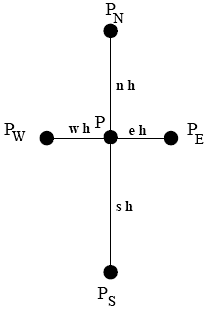
\includegraphics[width=3cm]{Content/02_numerics/irregulaereGitter.png}

\end{minipage}
\hfill
\begin{minipage}{14cm}

$- \frac{2}{h^2} \cdot \left(\frac{u(x+e \cdot h,y)-u(x,y)}{e(e+w)} +\frac{u(x-w \cdot h,y)-u(x,y)}{w(e+w)}+\frac{u(x,y+n \cdot h)-u(x,y)}{n(n+s)} + \frac{u(x,y-s \cdot h)-u(x,y)}{s(n+s)}\right)=f(x,y)$\\
\\
oder\\
\\
$- \frac{2}{h^2} \cdot \left(\frac{u(P_E) - u(P)}{e(e+w)} + \frac{u(P_W) - u(P)}{w(e+w)} + \frac{u(P_N) - u(P)}{n(n+s)} + \frac{u(P_S) - u(P)}{s(n+s)}\right) = f(x,y)$\\
\\
Wenn $\Delta x, \Delta y$ konstant ($w \cdot h = e \cdot h,\, n \cdot h = s \cdot h$) sowie $h=1$:\\
\\
$-\left(\frac{u(P_E) + u(P_W) - 2 u(P)}{\Delta x^2} + \frac{u(P_N) + u(P_S) - 2 u(P)}{\Delta y^2}\right) = f(x,y)$\\

\end{minipage}
\subsubsection{Neumann Rand
%$\partial_n u(x,y) \forall (x,y) \epsilon \partial_n G$
}
\begin{minipage}{4cm}
	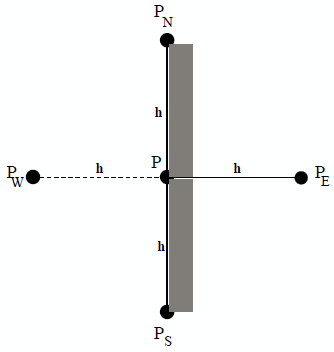
\includegraphics[width=4cm]{Content/02_numerics/NeumannRand.png}
\end{minipage}
\hfill
\begin{minipage}{14cm}
Bei Neumann Rand-Bedingungen müssen die Randpunkte ebenfalls berechnet werden.
In der Abbildung sind $P$, $P_N$ und $P_S$ auf dem Rand,
$P_E$ ist liegt innerhalb, und $P_W$ ausserhalb von $\Omega$.
Gegeben sei  die Neumannsche Randbedingung in $P$: $\boxed{\partFrac{u}{n}(P)=g(P)}$\\
Aus der Ableitung $u_x(P) = \partFrac{u}{n}(P) = \frac{u(P_E)-u(P_W)}{2h}$
kann der ausserhalb liegende Punkt $u(P_W)$ berechnet werden: $u(P_W)=u(P_E)-2h\cdot u_x(P)$.
Somit gilt:

$\boxed{\frac{2u(P_E) + u(P_N) +
u(P_S)- 4 u(P) - 2h\cdot u_x(P)}{h^2}}$\\

Sind $P_W$ und $P_E$ vertauscht, so ist das Vorzeichen umgekehrt:
$u(P_W)=u(P_E)+2h\cdot u_x(P)$.\\

\textbf{Spiegelmethode}:\\
Wenn $u_x(x,y) = 0$, dann spricht man auch von der Spiegelmethode. Die Punkte $P_W$ und $P_E$ weisen dann die gleiche Wertigkeit auf ($P_W=P_E$).
\end{minipage}


\subsection{FDM für parabolische PDGL}
	Wärmeleitungsgleichung: $\boxed{u_t(x,t)=u_{xx}(x,t)}$\qquad $f(0)=f(1)=0$ \qquad$ \overset{\_}{\Omega}=[0,1]\times [0,\infty]$\\

	Randbedingungen: $u(x,0)=f(x) \qquad u(0,t)=u(1,t)=0\qquad x\in(0,1) \qquad t\in[0,\infty)$

\newpage

\subsubsection{Explizites Verfahren (Richardson-Verfahren)}
$\boxed{\frac{\tilde{u}(x,t+\Delta t) - \tilde{u}(x,t)}{\Delta t} =
\frac{\tilde{u}(x+\Delta x, t)-2\tilde{u}(x,y) + \tilde{u}( x - \Delta x, t )} {\Delta x^2}} \qquad \Delta x=\frac{1}{n} \qquad \Delta t=\frac{r}{n^2} \qquad \boxed{r=\frac{\Delta
t}{\Delta x^2}}$\\

\textbf{Idee:} Aus den Positionen $k$ wird $k+1$ berechnet: $\tilde{u}_{j,k+1} = r \tilde{u}_{j-1,k} + (1-2r)\tilde{u}_{j,k} + r \tilde{u}_{j+1,k}$\\
Diskretisierung von t: k, k+1, \ldots\\
Diskretisierung von x: j, j+1, \ldots\\

\begin{itemize}
\item Initialisierung, Randbedingung: $\tilde{u}_{j,0}=f(j/n)$ \qquad $\tilde{u}_{0,k}=\tilde{u}_{n,k}=0$
\item Approximationsmatrize: $C^{(n)}=\tridiag_{n-1}(r,1-2r,r)=\begin{bmatrix}
1-2r& r		& 0		& 0 	&\cdots\\
r	& 1-2r  & r		& 0		&\cdots\\
0	& r		& 1-2r 	& r 	&\cdots\\
0	& 0		& r		& 1-2r 	&\cdots\\
\vdots&	\vdots&\vdots&\vdots&\ddots
\end{bmatrix}$
\item Einen Schritt berechnen: $\tilde{u}^{(k+1)}=C^{(n)} \tilde{u}^{(k)}$
\item $k$-Schritte berechnen: $\tilde{u}^{(k)}=\big\{C^{(n)}\big\}^k \tilde{u}^{(0)}$
\end{itemize}

\textbf{Konvergenzverhalten:} \\

\begin{minipage}{6cm}
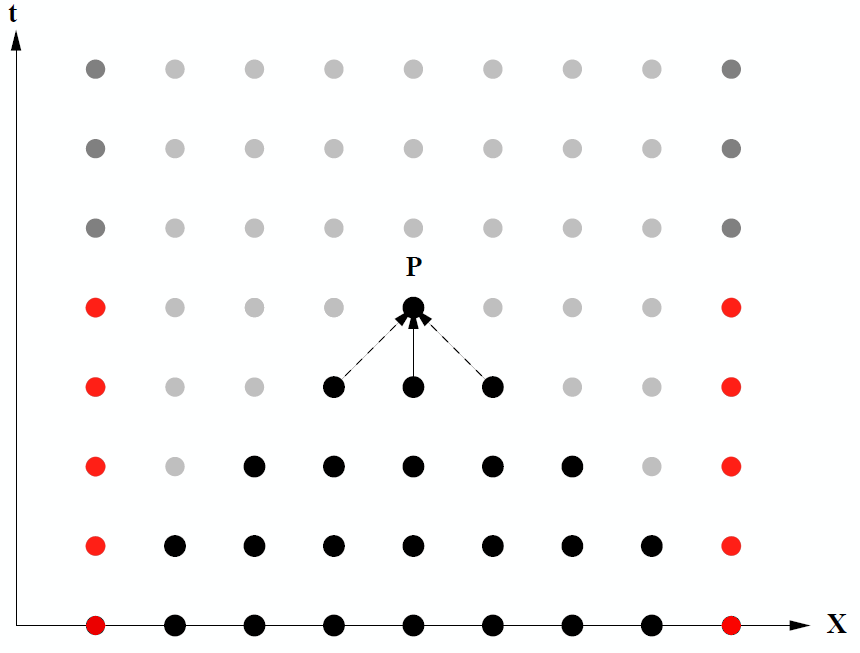
\includegraphics[width=6cm]{Content/02_numerics/KonvExplizit.png}
\end{minipage}
\hfill
\begin{minipage}{12cm}
Verfahren ist stabil wenn: $||C^{(n)}|| < 1 \qquad \Rightarrow\qquad r < \frac{1}{2}$\\

Dies macht es nötig, die Zeitschritte extrem klein zu wählen. Darum ist das Verfahren auch nicht wirklich praxistauglich, weil sehr hohe Rechenkapazität nötig sind.\\

Der Grund für das schlechte Konvergenzverhalten kann geometrisch visualisiert werden. In die Berechnung des Wertes im Knoten $P$, werden die Werte aller schwarz eingefärbter Knoten eingehen. Von den Randwerten wird nur die 0-te Stufe berücksichtigt.
\end{minipage}
Damit das Verfahren mit $C^k$ für k-Schritte berechnet werden kann, müssen die
rot eingefärbten Werte (links und rechts) gleich 0 sein (Boundary Condition).
Für den Randvektor $\tilde{u}^{(0)}$ werden nur die untersten schwarzen 7 Punkte
eingefüllt.

\subsubsection{Implizites Verfahren}
Im Unterschied zum expliziten Verfahren, das Werte vom vorherigen Zeitpunkt nutzt, wird hier das ein Gleichungssystem global gelöst.\\

$\boxed{\frac{\tilde{u}(x,t) - \tilde{u}(x,t -\Delta t)}{\Delta t} =
\frac{\tilde{u}(x+\Delta x, t)-2\tilde{u}(x,y) + \tilde{u}( x - \Delta x, t )} {\Delta x^2}}
 \qquad \Delta x=\frac{1}{n} \qquad \Delta t=\frac{r}{n^2} \qquad \boxed{r=\frac{\Delta
t}{\Delta x^2}}$\\

$ \tilde{u}_{j,k} = - r \tilde{u}_{j-1,k+1} + (1+2r)\tilde{u}_{j,k+1} - r \tilde{u}_{j+1,k+1}$

\textbf{Idee:} Die Ableitungen werden mittels Rückwärtsdifferenz berechnet\\


\begin{itemize}
\item Initialisierung, Randbedingung: $\tilde{u}_{j,0}=f(j/n)$ \qquad $\tilde{u}_{0,k}=\tilde{u}_{n,k}=0$
\item Approximationsmatrize: $E^{(n)}=\tridiag_{n-1}(-r,1+2r,-r)=\begin{bmatrix}
1+2r& -r		& 0		& 0 	&\cdots\\
-r	& 1+2r  & -r		& 0		&\cdots\\
0	& -r		& 1+2r 	& -r 	&\cdots\\
0	& 0		& -r		& 1+2r 	&\cdots\\
\vdots&	\vdots&\vdots&\vdots&\ddots
\end{bmatrix}$
\item Gleichung: $\tilde{u}^{(k)}=E^{(n)} \cdot \tilde{u}^{(k + 1)}$
\item Einen Schritt berechnen: $\tilde{u}^{(k+1)}=\left\{E^{(n)}\right\}^{-1} \tilde{u}^{(k)}$
\item $k$-Schritte berechnen: $\tilde{u}^{(k)}=\left\{E^{(n)}\right\}^{\bm{-}k} \tilde{u}^{(0)}$
\end{itemize}

\textbf{Vorteil:} Das implizite Verfahren ist immer stabil, unabhängig von der Zeitauflösung $\Delta t$\\
\textbf{Nachteil:} Aufwendige Matrixinversion nötig.

\subsubsection{Crank Nicolson -Verfahren (gemischtes Verfahren)}

Die Idee des Verfahrens von Crank-Nicolson ist es die beiden Approximationen

$\boxed{\frac{\tilde{u}(x,t+\Delta t) - \tilde{u}(x,t)}{\Delta t} =
\frac{\tilde{u}(x+\Delta x, t)-2\tilde{u}(x,t) + \tilde{u}( x - \Delta x, t )} {\Delta x^2}}$\\
$\boxed{\frac{\tilde{u}(x,t+\Delta t) - \tilde{u}(x,t)}{\Delta t} =
\frac{\tilde{u}(x+\Delta x, t+\Delta t)-2\tilde{u}(x,t+\Delta t) + \tilde{u}( x - \Delta x, t +\Delta t)} {\Delta x^2}}$

zu mitteln. Mit dieser Idee geht das stetige Problem in folgendes diskretes Problem über:

$-r \tilde{u}_{j-1,k+1} + (2+2r)\tilde{u}_{j,k+1} - r \tilde{u}_{j+1,k+1} = r
\tilde{u}_{j-1,k} + (2-2r)\tilde{u}_{j,k} + r \tilde{u}_{j+1,k} $

Wie bei den anderen Verfahren gilt: $\Delta x=\frac{1}{n} \qquad \Delta t=\frac{r}{n^2} \qquad \boxed{r=\frac{\Delta
t}{\Delta x^2}}$
\begin{itemize}
\item Initialisierung, Randbedingung: $\tilde{u}_{j,0}=f(j/n)$ \qquad $\tilde{u}_{0,k}=\tilde{u}_{n,k}=0$
\item Approximationsmatrizen:\\
$F^{(n)}=E^{(n)}+I=\tridiag_{n-1}(-r,2+2r,-r)=\begin{bmatrix}
2+2r& -r	& 0		& 0 	&\cdots\\
-r	& 2+2r  & -r	& 0		&\cdots\\
0	& -r	& 2+2r 	& -r 	&\cdots\\
0	& 0		& -r	& 2+2r 	&\cdots\\
\vdots&	\vdots&\vdots&\vdots&\ddots
\end{bmatrix}$\\
$G^{(n)}=C^{(n)}+I=\tridiag_{n-1}(~r,~2-2r,~r~)=\begin{bmatrix}
2-2r& r		& 0		& 0 	&\cdots\\
r	& 2-2r  & r		& 0		&\cdots\\
0	& r		& 2-2r 	& r 	&\cdots\\
0	& 0		& r		& 2-2r 	&\cdots\\
\vdots&	\vdots&\vdots&\vdots&\ddots
\end{bmatrix}$
\item Gleichung: $F^{(n)} \cdot \tilde{u}^{(k+1)}=G^{(n)} \cdot \tilde{u}^{(k)}$
\item Einen Schritt berechnen: $\tilde{u}^{(k+1)}=\left\{F^{(n)}\right\}^{-1} \cdot G^{(n)}\cdot \tilde{u}^{(k)}$
\item $k$-Schritte berechnen: $\tilde{u}^{(k)}=\left(\left\{F^{(n)}\right\}^{-1} \cdot G^{(n)}\right)^{k}\cdot \tilde{u}^{(0)}$
\end{itemize}

\subsection{FDM für Hyperbolische PDGL}

\begin{minipage}{8cm}
$u_{tt}=u_{xx} \rightarrow \text{homogen}$\\
$u_{tt} -u_{xx}= v(x,t) \rightarrow \text{inhomogen}$
\end{minipage}
\begin{minipage}{5cm}
Anfangsbedingungen:\\
$u(x,0)=f(x) \quad u_t(x,0)=g(x)$
\end{minipage}\\

\subsubsection{Leap-Frog-Schema}
$\tilde{u}_{j,k+1}=r^2 \tilde{u}_{j-1,k} + 2(1-r^2)\tilde{u}_{j,k}+ r^2
\tilde{u}_{j+1,k}-\tilde{u}_{j,k-1} \qquad r = \frac{\Delta t}{\Delta x}$\\
\\
$\tilde{u}_{j,0} = f(j\Delta x) \qquad \tilde{u}_{j,1}= f(j\Delta x) + g(j\Delta x)\Delta t + f''(j \Delta x) \frac{\Delta t^2}{2} $\\

\subsubsection{Transportgleichung}
$$u_x(x,t) + u_t(x, t) = 0 \qquad u(x,0)=f(x) \longrightarrow u(x,t)=f(x-t)$$


\subparagraph{Downwind Scheme}
$$\frac{\tilde{u}(x,t+\Delta t)-\tilde{u}(x,t)}{\Delta t} + \frac{\tilde{u}(x + \Delta x,t) - \tilde{u}(x, t)}{\Delta x} = 0 \qquad
\tilde{u}_{j,k+1}=(1+r)\tilde{u}_{j,k} - r\tilde{u}_{j+1,k} \quad r=\frac{\Delta t}{\Delta x} \quad \text{Meist Divergent}$$

\subparagraph{Upwind Scheme}
$$\frac{\tilde{u}(x,t+\Delta t)-\tilde{u}(x,t)}{\Delta t} + \frac{\tilde{u}(x,t) - \tilde{u}(x-\Delta x,
t)}{\Delta x} = 0 \qquad
\tilde{u}_{j,k+1}=(1-r)\tilde{u}_{j,k} + r\tilde{u}_{j-1,k} \quad \text{Konvergent für} \quad r=\frac{\Delta t}{\Delta x} \leq 1$$

\subparagraph{Centered Scheme}
$$\frac{\tilde{u}(x,t+\Delta t)-\tilde{u}(x,t)}{\Delta t} + \frac{\tilde{u}(x + \Delta x,t) - \tilde{u}(x - \Delta x, t)}{2 \Delta x} = 0 \qquad
\tilde{u}_{j,k+1}= - \frac{r}{2}\tilde{u}_{j+1,k} + \tilde{u}_{j,k} + \frac{r}{2}\tilde{u}_{j-1,k} \quad r=\frac{\Delta t}{\Delta x} $$


\subparagraph{Lax-Wendroff Scheme}
$$\tilde{u}_{j,k+1}=  A\tilde{u}_{j+1,k} + B \tilde{u}_{j,k} + C \tilde{u}_{j-1,k} \quad r=\frac{\Delta t}{\Delta x} \quad A = \frac{r^2 - r}{2} \quad B = 1- r^2 \quad C= \frac{r^2 +r}{2}$$

\subsection{FVM (Finite Volumen Methode, Verfahren von Voronoi)}
$\Delta u=0$\qquad in \quad$\Omega$\\
$u(x,y)=f(x,y)$ \qquad auf \quad$\partial\Omega$\\
Der Satz von Gauss sagt: $\boxed{\oint\limits_{\Gamma}{\Delta u(x,y) dx dy}=\int\limits_{\Gamma}{\mathrm{div}~\mathrm{grad}~ u(x,y) dx dy}=\oint\limits_{\partial\Gamma}{\mathrm{grad}~ u(x,y) d\vec{n}}}$\\


Wobei der Randnormalvektor $\vec{n}$ immer senkrecht gegen das Aussengebiet $\Gamma$ gerichtet wird.\\

$\Rightarrow$ $\oint\limits_{\Gamma}{\Delta u(x,y) dx dy}=\oint\limits_{\partial\Gamma}{\mathrm{grad}~ u(x,y) d\vec{n}}=0$

\begin{minipage}{4cm}
	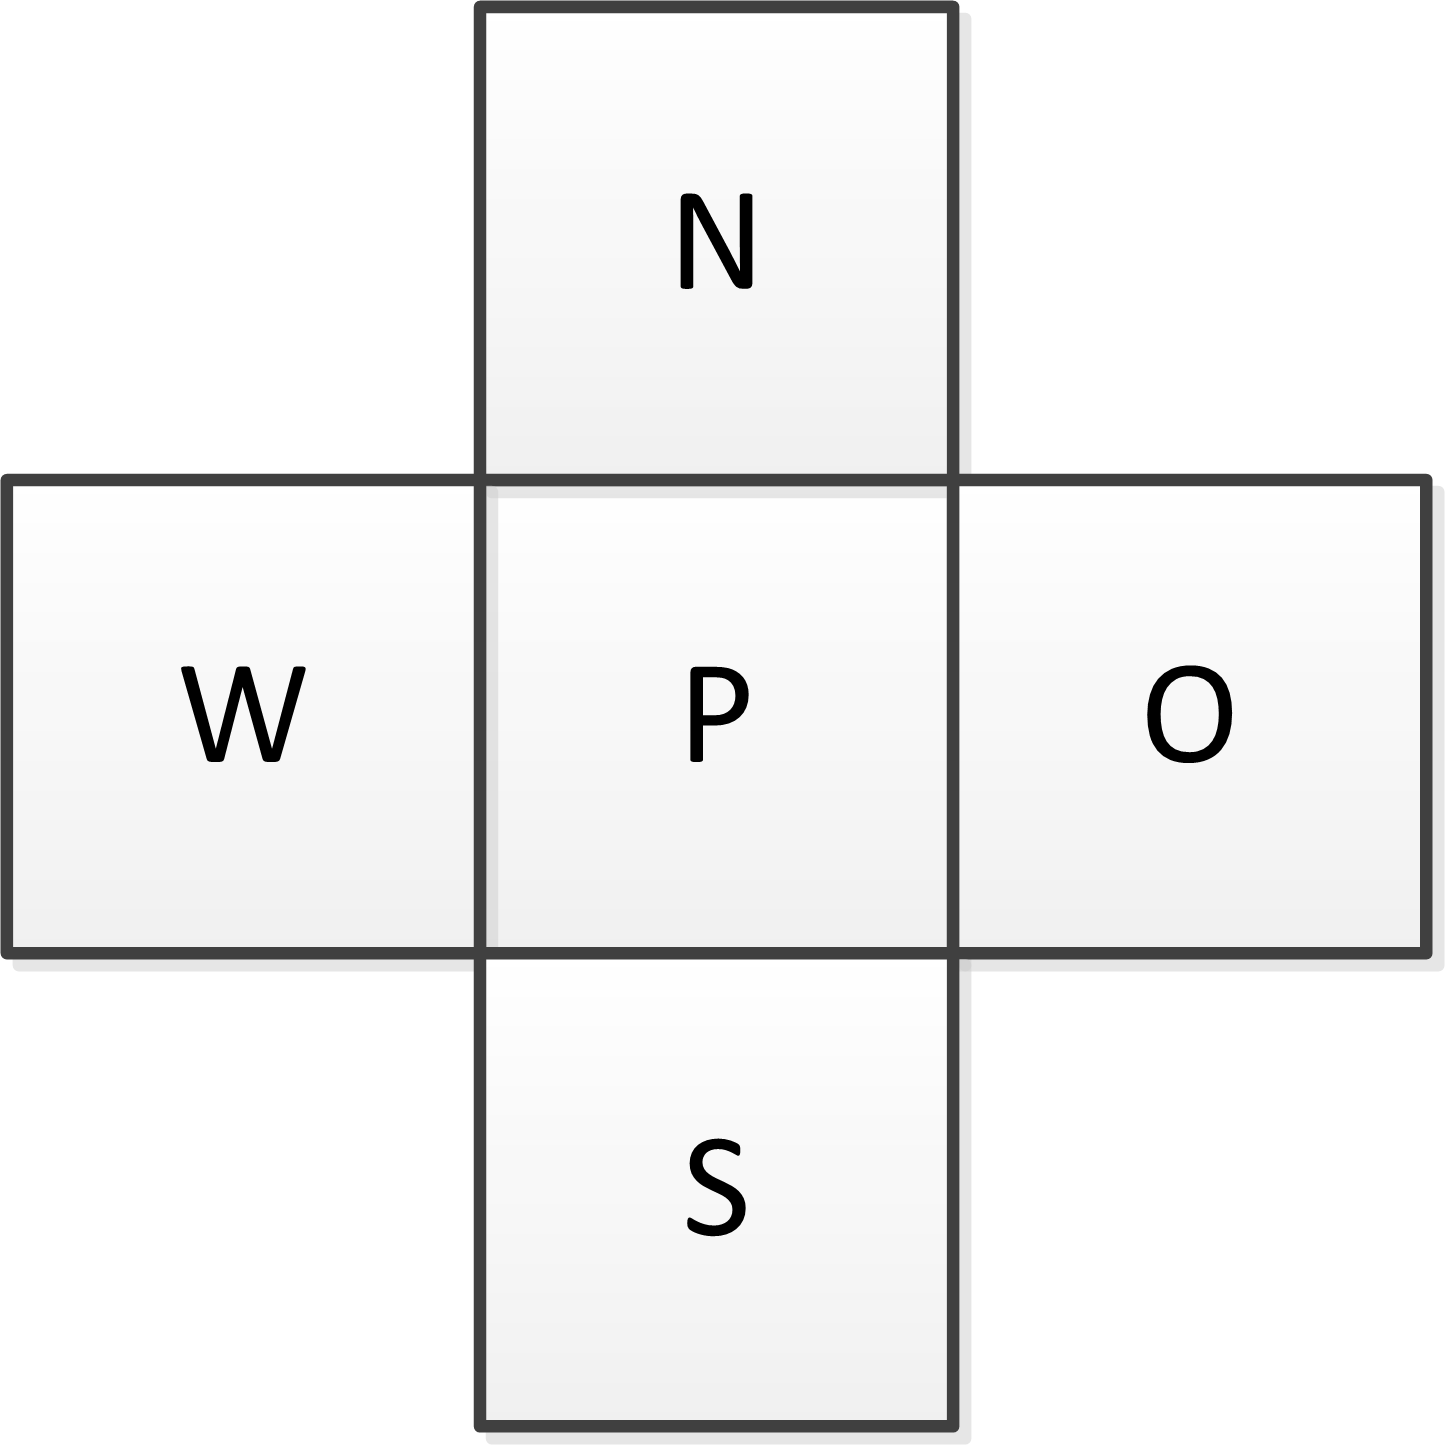
\includegraphics[width=4cm]{Content/02_numerics/FVMPrinzip.png}
\end{minipage}
\hfill
\begin{minipage}{14cm}
	$\frac{u(P_E)-u(P_P)}{h}\cdot h+\frac{u(P_N)-u(P_P)}{h}\cdot h+\frac{u(P_W)-u(P_P)}{h}\cdot h+\frac{u(P_S)-u(P_P)}{h}\cdot h\approx 0$\\

	$\Rightarrow\tilde{u}(P_E)+\tilde{u}(P_N)+\tilde{u}(P_W)+\tilde{u}(P_S)-4\cdot\tilde{u}(P_P)=0$
\end{minipage}

\textbf{Vorteile:}\\
\begin{itemize}
\item Man kann mit Flussgrössen und Bilanzen rechnen, dadurch kann der
Laplace-Operator $(\Delta)$ verzichtet werden und somit die aufwendige Mathematik umgangen werden.
\item Es kann mit komplizierten Geometrien gerechnet werden.
\end{itemize}

\begin{minipage}{6cm}
	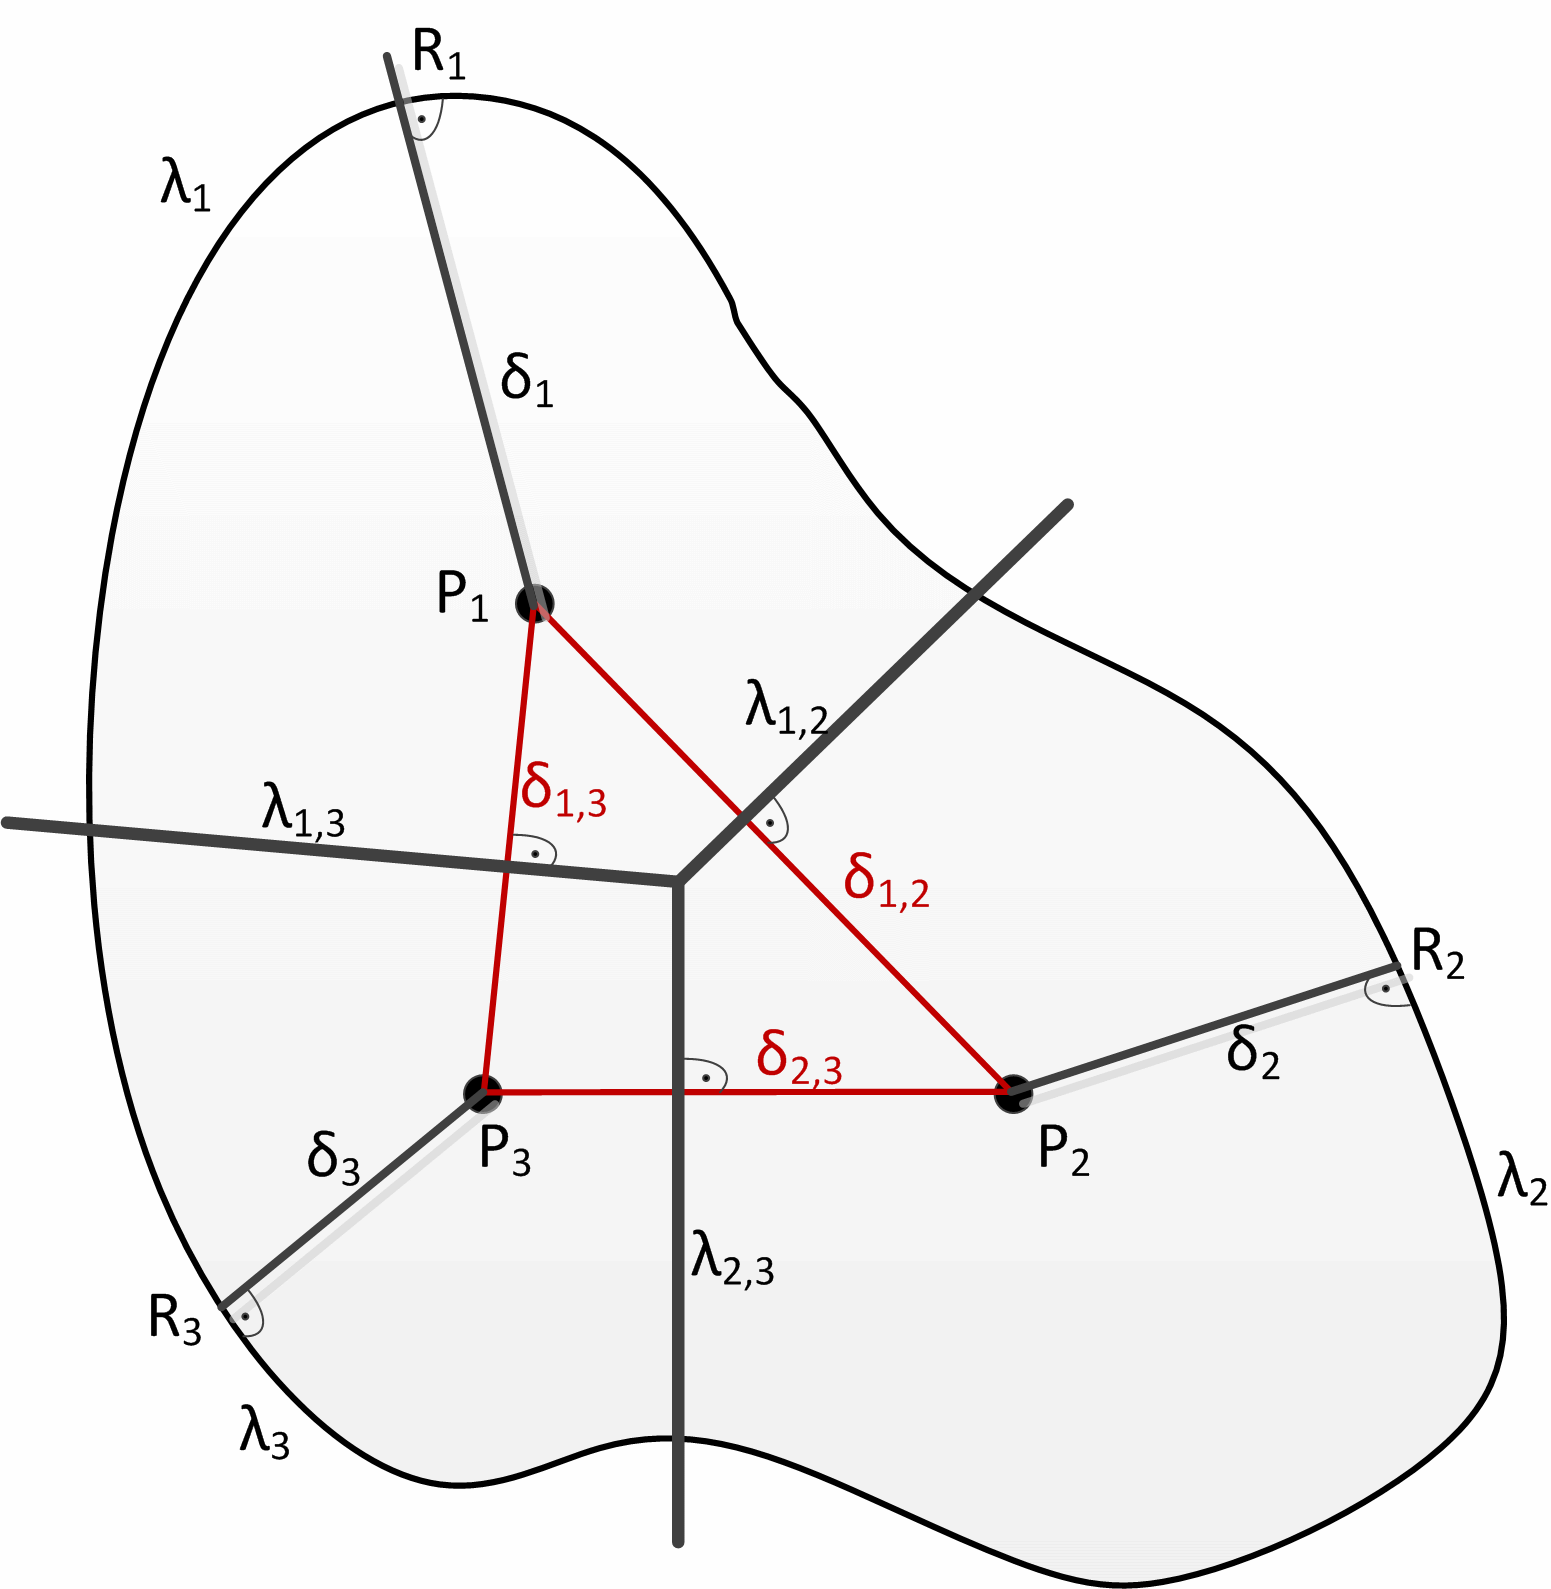
\includegraphics[width=6cm]{Content/02_numerics/FVM1.png}
\end{minipage}
\hfill
\begin{minipage}{12cm}
\textbf{Vorgehen bei der Berechnung:}\\
\begin{enumerate}
\item Punkte $P_1,\ldots,P_n$ wählen.
\item Aufteilen des Bereichs in kleine Teilbereiche, z.B. durch Mittelsenkrechte
\item Rand diskretisieren.\\
\end{enumerate}

Für $P_i$-Zelle: $\sum\limits_{j} \dfrac{u(P_{i,j}) - u(P_i)}{\delta_{i,j}} \cdot \lambda_{i,j} = 0$

Für P1-Zelle:\quad $\frac{\tilde{u}(P_2)-\tilde{u}(P_1)}{\delta_{1,2}}\cdot\lambda_{1,2}+\frac{\tilde{u}(P_3)-\tilde{u}(P_1)}{\delta_{1,3}}\cdot\lambda_{1,3}+\frac{\tilde{u}(R_1)-\tilde{u}(P_1)}{\delta_1}\cdot\lambda_1=0$\\

Für P2-Zelle:\quad $\frac{\tilde{u}(P_1)-\tilde{u}(P_2)}{\delta_{1,2}}\cdot\lambda_{1,2}+\frac{\tilde{u}(P_3)-\tilde{u}(P_2)}{\delta_{2,3}}\cdot\lambda_{2,3}+\frac{\tilde{u}(R_2)-\tilde{u}(P_2)}{\delta_2}\cdot\lambda_2=0$\\

Für P3-Zelle:\quad $\frac{\tilde{u}(P_2)-\tilde{u}(P_3)}{\delta_{2,3}}\cdot\lambda_{2,3}+\frac{\tilde{u}(P_1)-\tilde{u}(P_3)}{\delta_{1,3}}\cdot\lambda_{1,3}+\frac{\tilde{u}(R_3)-\tilde{u}(P_3)}{\delta_3}\cdot\lambda_3=0$\\
\end{minipage}

\begin{minipage}{6cm}
	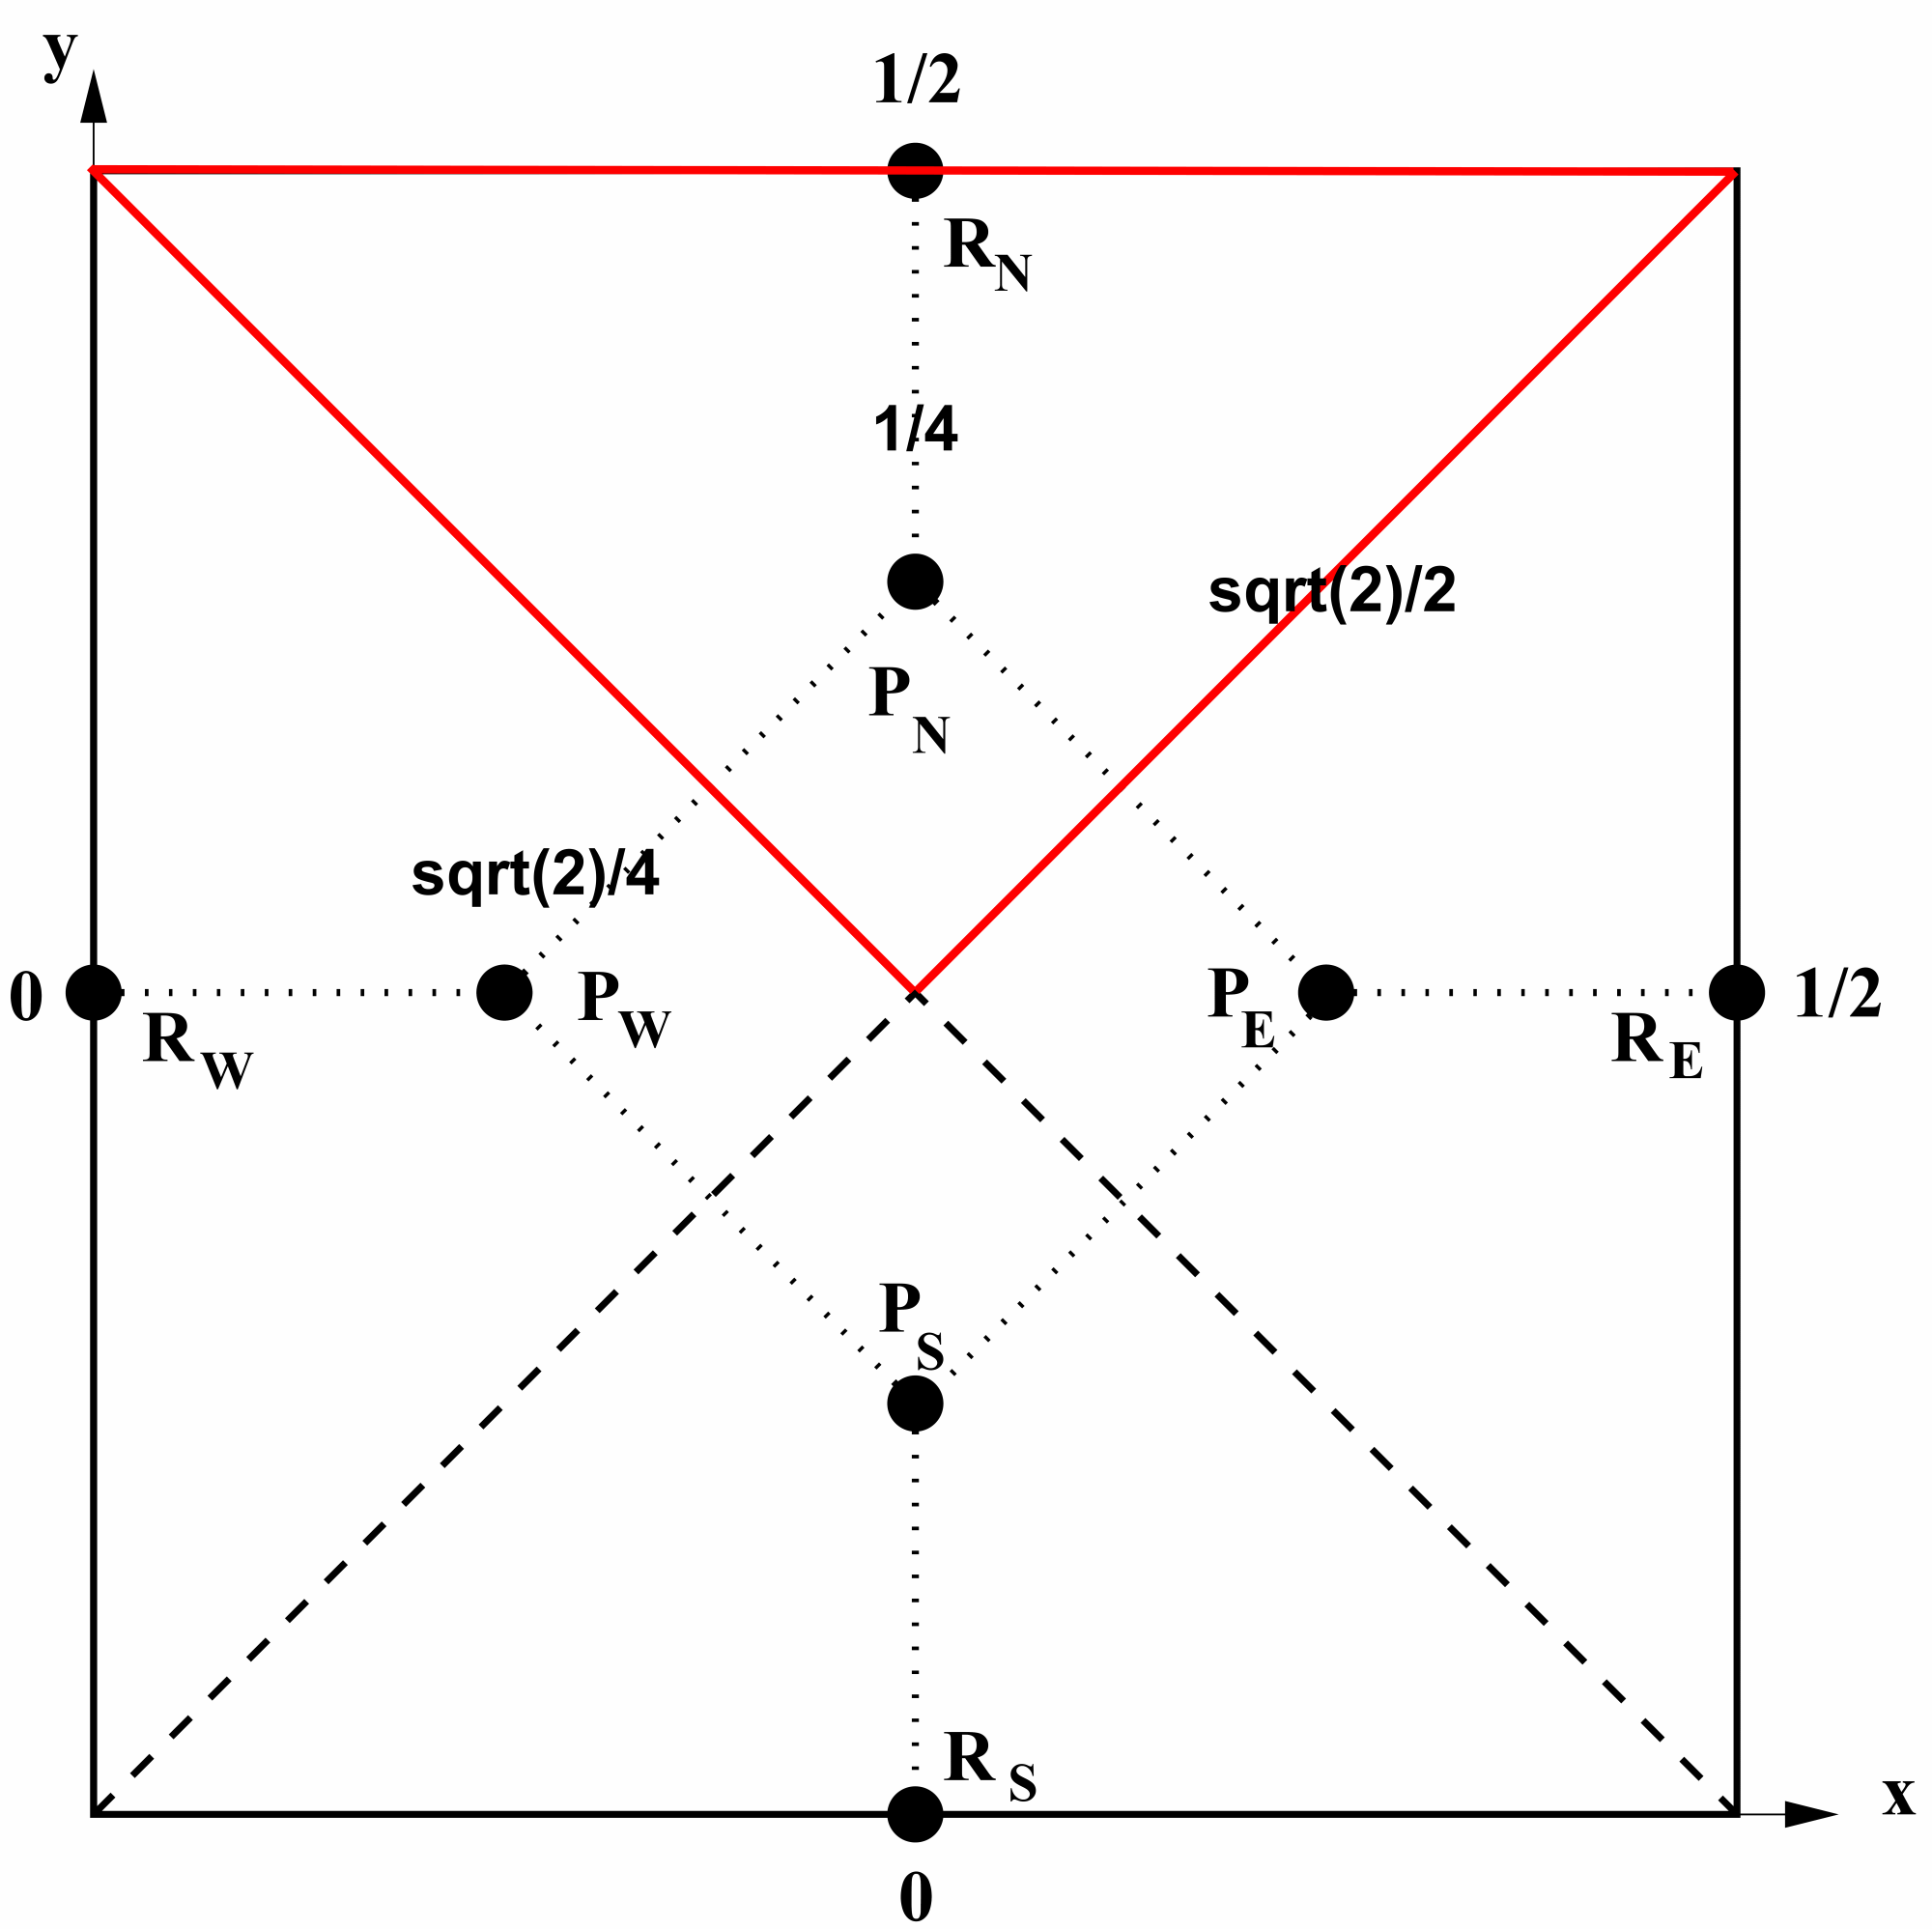
\includegraphics[width=6cm]{Content/02_numerics/FVM2.png}
\end{minipage}
\hfill
\begin{minipage}{12cm}

 $\frac{\tilde{u}(P_E)-\tilde{u}(P_N)}{1/4\cdot\sqrt{2}}\cdot\frac{\sqrt{2}}{2}+\frac{\tilde{u}(P_W)-\tilde{u}(P_N)}{1/4\cdot\sqrt{2}}\cdot\frac{\sqrt{2}}{2}+\frac{\tilde{u}(R_N)-\tilde{u}(P_N)}{1/4}\cdot 1=0$\\

 $(\tilde{u}_E-\tilde{u}_N)\cdot 2 + (\tilde{u}_W-\tilde{u}_N)\cdot 2 + (1/2-\tilde{u}_N)\cdot 4=0$\\

 $0\cdot\tilde{u}_S+2\cdot\tilde{u}_E+2\cdot\tilde{u}_W-8\cdot\tilde{u}_N+2=0$


\end{minipage}

\begin{minipage}{6cm}
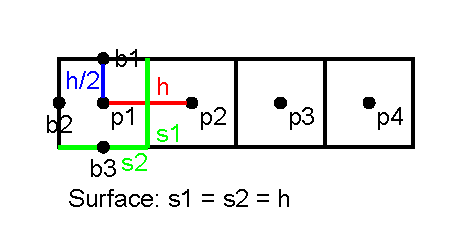
\includegraphics[width=6cm]{Content/02_numerics/fvm_beispiel.pdf}
\end{minipage}
\hfill
\begin{minipage}{12cm}

u1: $\frac{u(b_1) - u(p_1)}{h/2} \cdot h + \frac{u(b_2) - u(p_1)}{h/2} \cdot h +
\frac{u(b_3) - u(p_1)}{h/2} \cdot s_2 + \frac{u(p_2) - u(p_1)}{h} \cdot s_1 $\\
\colorbox{yellow}{Achtung wenns schnell gehen muss: $\frac{u(b_2) - u(p_1)}{h/2}
\cdot h = (u(b_2) - u(p_1)) \cdot 2$}

\end{minipage}

example with $\Delta u(x,y) \neq 0$ and two voronoi points: \\
The function $u(x,y)$ is defined on the square $\Omega =[0,3]\times [0,3]$. The function $u(x,y)$ satisfies in $\Omega$ $$  \Delta u(x,y)+4=0 $$ and $u(x,y)=0$ on the boundary of $\Omega$. Determine approximate values for $u(1,1)$ and $u(2,2)$. Use finite volumes à la Voronoi with Voronoi-points $(1,1)$ and $(2,2)$


\begin{minipage}{6cm}
  \begin{tikzpicture}

    \draw[thick,-latex] (0,0) -- (3.3,0) node[anchor=north](){${x}$};
    \draw[thick,-latex] (0,0) -- (0,3.3) node[anchor= west](){${y}$};


    \foreach \x in {0,1,...,3}  {   % for x-axis
      \draw [] (\x,0) -- (\x,-0.1) node[anchor=north](){0};
      \draw [] (0,\x) -- (-0.1,\x)  node[anchor=east](){0};
      \node[anchor=center] () at (\x,0) {\textbullet};
      \node[anchor=center] () at (0, \x) {\textbullet};
      \node[anchor=center] () at (3, \x) {\textbullet};
      \node[anchor=center] () at (\x, 3) {\textbullet};
    }


    \node[anchor=center, red] () at (1, 1) {\textbullet};
    \node[anchor=center, red] () at (2, 2) {\textbullet};
    \node[anchor=west, red] () at (1, 1) {$\tilde u_1$};
    \node[anchor=east, red] () at (2, 2) {$\tilde u_2$};

    \draw[green, thick] (1, 1) -- (2, 2);
    \draw[red, thick] (0, 0) -- (0, 3);
    \draw[red, thick] (0, 0) -- (3, 0);
    \draw[red, thick] (3, 0) -- (3, 3);
    \draw[red, thick] (0, 3) -- (3, 3);
    \draw[blue, thick] (1,1) -- (0,1);
    \draw[blue, thick] (2,2) -- (3,2);
    \draw[green, thick] (0,3) -- (3,0);


  \end{tikzpicture}

\end{minipage}
\hfill
\begin{minipage}{12cm}
$$ \frac{1}{2} \int_{0}^{3} \int_{0}^{3} -4 \,dxdy = -18 $$
Function integrated over the voronoi cell example 68 in the script
$$
\frac{0-\tilde u_1}{\textcolor{blue}{1}} \textcolor{red}{6} + \frac{\tilde u_2  -\tilde u_1}{\textcolor{green}{\sqrt{2}}} \textcolor{green}{3\sqrt{2}} = -18
$$
$$
\frac{0-\tilde u_2}{\textcolor{blue}{1}} \textcolor{red}{6} + \frac{\tilde u_1 -\tilde u_2}{\textcolor{green}{\sqrt{2}}} \textcolor{green}{3\sqrt{2}} = -18$$

$$ A = \begin{bmatrix}
-9 &  3\\
3 & -9
\end{bmatrix} \begin{pmatrix}
\tilde u_1 \\
\tilde u_2
\end{pmatrix}= \begin{pmatrix}
-18 \\
-18
\end{pmatrix}
$$


\end{minipage}


\clearpage
\section{FEM}

Der Vektorraum $\mathbb{V}$ hat undendlich viele Dimensionen. Falls wir n unabhängige Funktionen $v_1,\ldots,v_n$ wählen, dann spannen die Funktionen $a_1\cdot v_1(x)+\ldots+a_n\cdot v_n(x)$ einen n dimensionalen Teilraum $\mathbb{V}^{(n)}$  von $\mathbb{V}$ auf. Dabei gilt:\\

$\boxed{\tilde{u}^{(n)}=a_1\cdot v_1(x)+\ldots+a_n\cdot v_n(x)}$
\subsection{Das Verfahren von Ritz}
\textbf{Ritzsche Matrize: }
$R^{(n)}=\begin{bmatrix}
	R_{1,1}& R_{1,2}&\cdots\\
	R_{2,1}& R_{2,2}&\cdots\\
	\vdots & \vdots &\ddots\\
\end{bmatrix}$ \qquad mit \qquad $R_{j,k}^{(n)}=\int\limits_{0}^{1}{v_j'(x)\cdot
v_k'(x) dx}$\\
\textbf{Ritzscher Vektor: } 
$r^{(n)}=\begin{bmatrix}
	r_1\\
	r_2\\
	\vdots\\
\end{bmatrix}$ \qquad mit \qquad $r_{k}^{(n)}=\int\limits_{0}^{1}{f(x)\cdot v_k(x) dx}$\\

\textbf{Lösung nach Ritz:} $R^{(n)}\cdot a=r^{(n)}\qquad \Rightarrow \qquad a=\left\{R^{(n)}\right\}^{-1}\cdot r^{(n)}$
\subsection{Das Verfahren von Galerkin}
\textbf{Galerksche Matrize: }
$G^{(n)}=\begin{bmatrix}
	G_{1,1}& G_{1,2}&\cdots\\
	G_{2,1}& G_{2,2}&\cdots\\
	\vdots & \vdots &\ddots\\
\end{bmatrix}$ \qquad mit \qquad $G_{j,k}^{(n)}=\int\limits_{0}^{1}{\underbrace{(v_j''(x))}_{v_j \text{ in Form von DGL!}}\cdot v_k(x) dx}$\\
\textbf{Galerkscher Vektor: } 
$g^{(n)}=\begin{bmatrix}
	g_1\\
	g_2\\
	\vdots\\
\end{bmatrix}$ \qquad mit \qquad $g_{k}^{(n)}=\int\limits_{0}^{1}{f(x)\cdot v_k(x) dx}$\\

\textbf{Lösung nach Galerkin:} $G^{(n)}\cdot a+g^{(n)}=0\qquad \Rightarrow
\qquad a=\textcolor{red}{\mathbf{-}}\left\{G^{(n)}\right\}^{-1}\cdot g^{(n)}$ \quad nach Ritz $G^{(n)} = -R^{(n)} \quad g^{(n)} = r^{(n)}$\\

Die obige Matrix ist nur für die PDGL $-u''(x) = f(x)$ mit dem Ansatz
$\tilde{u}(x) = a_1 \cdot v_1(x) + a_2 \cdot v_2(x)$ gültig. Ansonsten muss ein
Gleichungssystem für $v_k$ = $v_1$ und $v_2$ aufgestellt werden (Beispiel
für DGL: $u''(x) + u(x) + x = 0$):\\
$\int\limits_{0}^{1}{(a_1 \cdot v_1''(x) + a_2 \cdot v_2''(x) + a_1 \cdot
v_1(x) + a_2 \cdot v_2(x) + x) \cdot v_k(x) dx} = 0 \rightarrow G_{j,k}^{(n)}=\int\limits_{0}^{1}(v_j''(x) + v_j(x))\cdot v_k(x) dx$

\subsection{Gewichtete Residuen}
Gewichtungsfunktionen: $\{w_1(x),\ldots,w_n(x)\}$

\textbf{Matrize (gewichtete Residuen): }
$M^{(n)}=\begin{bmatrix}
	M_{1,1}& M_{1,2}&\cdots\\
	M_{2,1}& M_{2,2}&\cdots\\
	\vdots & \vdots &\ddots\\
\end{bmatrix}$ \qquad mit \qquad $M_{j,k}^{(n)}=\int\limits_{0}^{1}{v_j''(x)\cdot w_k(x) dx}$\\
\textbf{Vektor (gewichtete Residuen): } 
$m^{(n)}=\begin{bmatrix}
	m_1\\
	m_2\\
	\vdots\\
\end{bmatrix}$ \qquad mit \qquad $m_{k}^{(n)}=\int\limits_{0}^{1}{f(x)\cdot w_k(x) dx}$\\

\textbf{Lösung der gewichteten Residuen:} $M^{(n)}\cdot a+m^{(n)}=0\qquad \Rightarrow \qquad a=\textcolor{red}{\mathbf{-}}\left\{M^{(n)}\right\}^{-1}\cdot m^{(n)}$

\subsection{Punktkollokation}
Im Sinne einer Punktkollokation (einzelne Punkte müssen zwischen wahrem Resultat und Approximation übereinstimmen) werden $n$ Stützstellen im Intervall von $[0,1]$ gewählt.\\

$\begin{bmatrix}
	v_1''(x_1)& v_2''(x_1)&\cdots\\
	v_1''(x_2)& v_2''(x_2)&\cdots\\
	\vdots& \vdots&\ddots
\end{bmatrix}\cdot
\begin{bmatrix}
a_1\\
a_2\\
\vdots
\end{bmatrix}
=\begin{bmatrix}
-f(x_1)\\
-f(x_2)\\
\vdots
\end{bmatrix}$\qquad Das Gleichungssystem nach a auflösen\\

Die obige Matrix ist nur für die PDGL $-u''(x) = f(x)$ mit dem Ansatz
$\tilde{u}(x) = a_1 \cdot v_1(x) + a_2 \cdot v_2(x)$ gültig. Ansonsten muss die
DGL mit den Ansatzfunktionen aufgestellt und an beiden Punkten eingesetzt
werden, um $a_1$ und $a_2$ zu bestimmen:\\
DGL: $u''(x) + u(x) = -x$ $\Rightarrow$ Gleichung an Punkt 1: $a_1 \cdot
v_1''(x_1) + a_2 \cdot v_2''(x_1) + a_1 \cdot v(x_1) + a_2 \cdot v(x_1) = - x_1$




\subsection{Bereichskollokation}
Im Gegensatz zur Punktkollokation müssen nicht einzelne Punkte sondern ganze Bereiche (Intervalle $I_k$) übereinstimmen. Für $-u''(x) = f(x)$ wird dieses Gleichungssystem aufgestellt.

$\begin{bmatrix}
	\int_{I_1} v_1'' & \int_{I_1} v_2''& \cdots\\
	\int_{I_2} v_1'' & \int_{I_2} v_2''& \cdots\\
	\vdots& \vdots&\ddots
\end{bmatrix}\cdot
\begin{bmatrix}
a_1\\
a_2\\
\vdots
\end{bmatrix}
=\begin{bmatrix}
-\int_{I_1} f(x)\\
-\int_{I_2} f(x)\\
\vdots
\end{bmatrix}$\qquad Das Gleichungssystem nach a auflösen


\subsection{Das Verfahren von Gauss (MSE)}

\textbf{Gausscher Matrize: }
$Q^{(n)}=\begin{bmatrix}
	Q_{1,1}& Q_{1,2}&\cdots\\
	Q_{2,1}& Q_{2,2}&\cdots\\
	\vdots & \vdots &\ddots\\
\end{bmatrix}$ \qquad mit \qquad $Q_{j,k}^{(n)}=\int\limits_{0}^{1}{v_j''(x)\cdot v_k''(x) dx}$\\
\textbf{Gausscher Vektor: } 
$q^{(n)}=\begin{bmatrix}
	q_1\\
	q_2\\
	\vdots\\
\end{bmatrix}$ \qquad mit \qquad $q_{k}^{(n)}=\int\limits_{0}^{1}{f(x)\cdot v_k''(x) dx}$\\

\textbf{Lösung nach Gauss:} $Q^{(n)}\cdot a+q^{(n)}=0\qquad \Rightarrow \qquad a=\textcolor{red}{\mathbf{-}}\left\{Q^{(n)}\right\}^{-1}\cdot q^{(n)}$

\subsection{Finite Elemente}

Die besprochenen Verfahren setzen die Wahl eines Satzes $v_1(x),\ldots,v_n(x)$ von Grundfunktionen voraus. Bei FEM wird mit lokalen Trägern (Grundfunktionen) gearbeitet, diese sind nur auf einem kleinen Intervall ungleich null. Der Vorteil dieses Vorgehens liegt darin, dass in einem Bereich nur ein Träger die Approximationsfunktion beeinflusst. Der Nachteil liegt in der hohen Anzahl der so benötigten Träger.\\

\textbf{WICHTIG:} Alle Verfahren werden mit einer Diskretisierung von $h=1/3$
vorgestellt.

\subsubsection{Knotenvariablen}
Als erstes werden auf dem Intervall $[0,1]$ $n$, normalerweise gleichverteilte, Knotenstellen eingeführt.

\begin{minipage}{11cm}
Dadurch wird das Intervall $[0,1]$ in Teilintervalle (Maschen) zerlegt.\\
 
Für $n=3$:\quad $I_1=[0,1/3]$\quad $I_1=[1/3,2/3]$\quad $I_1=[2/3,1]$\\

Als nächstes wird jeder Knotenstelle $x_k$ eine Ansatzvariable (Knotenvariable) zugeordnet.\\

Ansatz: \quad $\tilde{u}(0)=a_0$\quad $\tilde{u}(1/3)=a_1$\quad $\tilde{u}(2/3)=a_2$\quad $\tilde{u}(1)=a_3$\\

Zusatzbedingungen:
\begin{tabular}{llll}
$v_0(0)=1$&$v_0(1/3)=0$&$v_0(2/3)=0$&$v_0(1)=0$\\
$v_1(0)=0$&$v_1(1/3)=1$&$v_1(2/3)=0$&$v_1(1)=0$\\
$v_2(0)=0$&$v_2(1/3)=0$&$v_2(2/3)=1$&$v_2(1)=0$\\
$v_3(0)=0$&$v_3(1/3)=0$&$v_3(2/3)=0$&$v_3(1)=1$\\
\end{tabular}
\end{minipage}
\hfill
\begin{minipage}{8cm}
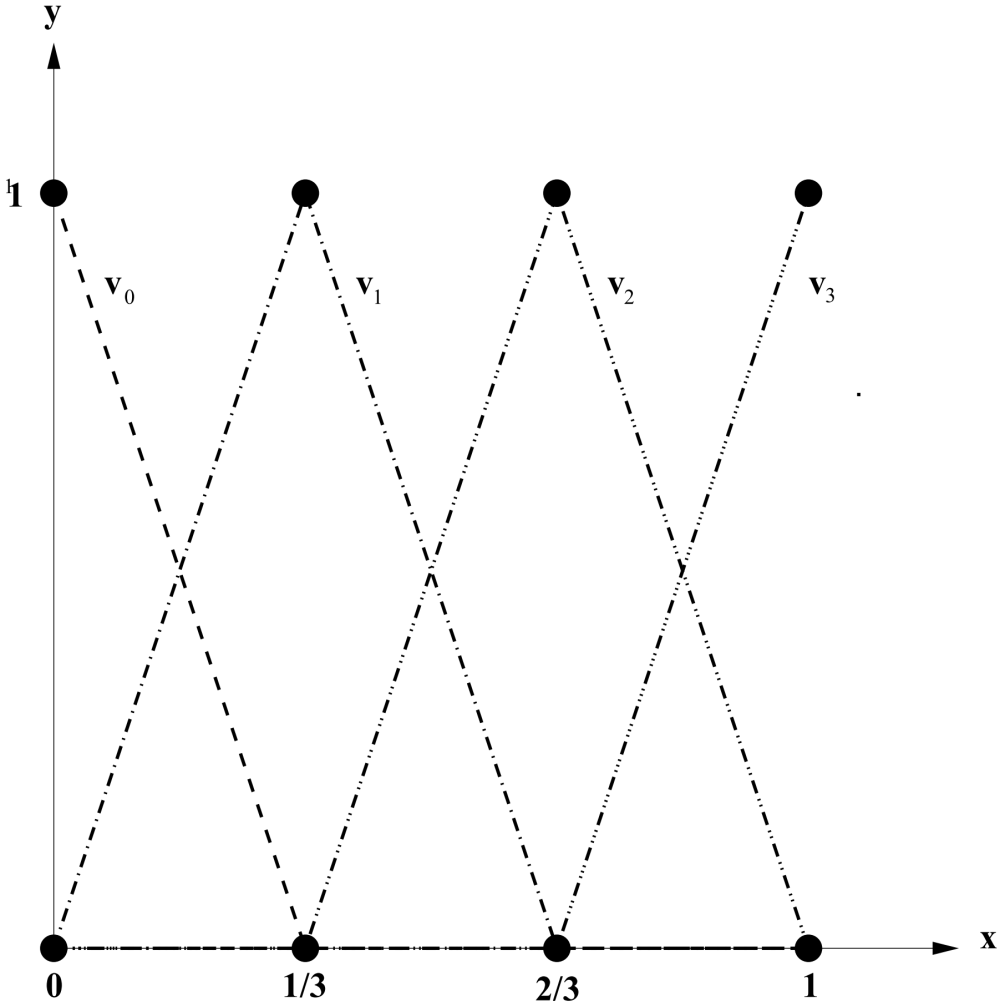
\includegraphics[width=8cm]{Content/02_numerics/Traeger1.png}
\end{minipage}


\subsubsection{Formfunktionen}
Die lokalen Grundfunktionen sollen aus Teilstücken einfacher Funktionen, z.B: Polynomen, die nur auf einer einzelnen Masche definiert sind zusammengesetzt werden.\\
Zwei mögliche Formfunktionen sind Beispielsweise:\quad $l_1(x)=1-x$\quad und \quad $l_2(x)=x$\\

\begin{minipage}{8cm}
	\begin{tabular}{lc|c|c}
	$t\in$&$[0,1/3]$&$[1/3,2/3]$&$[2/3,1]$\\
	\hline
	$v_0=$&$1-3x$&$0$&$0$\\
	$v_1=$&$3x$&$2-3x$&$0$\\
	$v_2=$&$0$&$-1+3x$&$3-3x$\\
	$v_3=$&$0$&$0$&$-2+3x$\\
	\end{tabular}
\end{minipage}
\hfill
\begin{minipage}{2cm}
$\Longrightarrow$
\end{minipage}
\hfill
\begin{minipage}{8cm}
	\begin{tabular}{lc|c|c}
	$t\in$&$[0,1/3]$&$[1/3,2/3]$&$[2/3,1]$\\
	\hline
	$v_0=$&$l_1(3x)$&$0$&$0$\\
	$v_1=$&$l_2(3x)$&$l_1(3x-1)$&$0$\\
	$v_2=$&$0$&$l_2(3x-1)$&$l_1(3x-2)$\\
	$v_3=$&$0$&$0$&$l_2(3x-2)$\\
	\end{tabular}
\end{minipage}
\subsubsection{Elementmatrizen}
Grundsätzlich kann die Ansatzvariable durch jedes Verfahren bestimmt werden.
Weil bei einer linearen Ansatzfunktion die zweite Ableitung trivial $(=0)$ ist die Wahl des Ritzschen Verfahren erzwungen.

Die Integrale werden maschenweise ausgewertet:\\

 $\int\limits_{0}^{1}{}=\int\limits_{0}^{1/3}{}+\int\limits_{1/3}^{2/3}{}+\int\limits_{2/3}^{1}{}$\\
 
Durch diesen Ansatz wird die Ritzsche Matrize über jede Masche einzeln berechnet und danach zur globalen Ritzschen Matrize aufsummier:\\

\qquad $R^{(4)}=R^{(4,1)}+R^{(4,2)}+R^{(4,3)}=
\begin{bmatrix}
	* & * & 0 & 0\\
	* & * & 0 & 0\\
	0 & 0 & 0 & 0\\
	0 & 0 & 0 & 0\\
\end{bmatrix}+
\begin{bmatrix}
	0 & 0 & 0 & 0\\
	0 & * & * & 0\\
	0 & * & * & 0\\
	0 & 0 & 0 & 0\\
\end{bmatrix}+
\begin{bmatrix}
	0 & 0 & 0 & 0\\
	0 & 0 & 0 & 0\\
	0 & 0 & * & *\\
	0 & 0 & * & *\\
\end{bmatrix}
$\\

Die mit $*$ bezeichneten $2\times 2$ Matrizen heissen Maschenmatrizen:\\

$M^{(4,1)}=M^{(4,2)}=M^{(4,3)}=
\begin{bmatrix}
	* & *\\
	* & *\\
\end{bmatrix}=3\cdot\begin{bmatrix}
	-1 & 1\\
	1 & -1\\
\end{bmatrix}\qquad\Rightarrow\qquad\boxed{M=\frac 1h\cdot
\underset{\text{\textbf{E}: Elementmatrize}}{\underbrace{\begin{bmatrix}
	-1 & 1\\
	1 & -1\\
\end{bmatrix}}}=\frac 1h\cdot \mathbf{E}}$\\

Die Elementmatrize wird nun in die entsprechende Ritzsche Matrize eingesetzt und überlagert. Für die Quantisierung von $h=1/3$ ergibt sich:\\

$R^{4}=
\begin{bmatrix}
	-3 & 3 & 0 & 0 \\
	3 & -3-3 & 3 & 0 \\
	0 & 3 & -3-3 & 3 \\
	0 & 0 & 3 & -3 \\
\end{bmatrix}=
\begin{bmatrix}
	-3 & 3 & 0 & 0 \\
	3 & -6 & 3 & 0 \\
	0 & 3 & -6 & 3 \\
	0 & 0 & 3 & -3 \\
\end{bmatrix}$\\

Der Ritzsche Vektor muss mittels Integration berechnet werden:\\

$r^4=
\begin{bmatrix}
	\int\limits_{0}^{1}{f(x)\cdot v_0(x)dx}\\
	\int\limits_{0}^{1}{f(x)\cdot v_1(x)dx}\\
	\int\limits_{0}^{1}{f(x)\cdot v_2(x)dx}\\
	\int\limits_{0}^{1}{f(x)\cdot v_3(x)dx}\\
\end{bmatrix}$\\

Das Ritzsche Gleichungssystem dazu ist: $\boxed{R^4\cdot a+r^4=0} \qquad\Rightarrow\qquad a=-\left\{R^4\right\}^{-1}\cdot r^4$\\

\textbf{Anfangsbedingungen:} Die Anfangsbedingungen $a_0$ und $a_n$ können direkt eingesetzt werden.\\

$a_0=10$\qquad$a_3=20$\\

$
	\begin{bmatrix}
		3 & -6 & 3 & 0 \\
		0 & 3 & -6 & 3 \\
	\end{bmatrix}\cdot
	\begin{bmatrix}
		10\\a_1\\a_2\\20
	\end{bmatrix}+r^4=0\qquad\Rightarrow\qquad
	\begin{bmatrix}
		-6 & 3 \\
		 3 & -6 \\
	\end{bmatrix}\cdot
	\begin{bmatrix}
		a_1\\a_2
	\end{bmatrix}+
	\begin{bmatrix}
		30\\60
	\end{bmatrix}+
	r^4=0
$\\

$
	\begin{bmatrix}
			a_1\\a_2
	\end{bmatrix}=
	\begin{bmatrix}
		-6 & 3 \\
	 	 3 & -6 \\
	\end{bmatrix}^{-1}\cdot
	\begin{bmatrix}
		-\left(r^4_1+3\cdot a_0\right)\\
		-\left(r^4_2+3\cdot a_3\right)\\
	\end{bmatrix}		
$

\subsubsection{Die Finite Elemente Handrechnung}
\textbf{Problemstellung:} $u''(x)+f(x)=0\qquad f(x)=20\qquad u(0)=10\qquad u(1)=20$\\

Die Approximation soll auf den \textbf{NICHT} gleichverteilten Intervallen: $[0,1/6]$,\quad $[1/6,1/2]$,\quad $[1/2,1]$\\

Die Entsprechenden Elementmatrizen E sind:\\

$
	\frac{1}{1/6}\begin{bmatrix}
		-1 & 1\\
		1 & -1
	\end{bmatrix}=
	\begin{bmatrix}
			-6 & 6\\
			6 & -6
	\end{bmatrix}\qquad
	\frac{1}{1/2-1/6}\begin{bmatrix}
		-1 & 1\\
		1 & -1
	\end{bmatrix}=
	\begin{bmatrix}
		-3 & 3\\
		3 & -3
	\end{bmatrix}\qquad
	\frac{1}{1-1/2}\begin{bmatrix}
		-1 & 1\\
		1 & -1
	\end{bmatrix}=
	\begin{bmatrix}
		-2 & 2\\
		2 & -2
	\end{bmatrix}
$\\
\\

\begin{minipage}{10cm}
Der Ritzsche Vektor und die Ritzsche Matrize sind:\\

$R^n=
\begin{bmatrix}
		-6 & 6 & 0 & 0\\
		6 & -9 & 3 & 0\\
		0 & 3 & -5 & 2\\
		0 & 0 & 2 & -2\\
\end{bmatrix}$

$
r^n=\begin{bmatrix}
		\int\limits_{0}^{1/6}{f(x)\cdot(1-6x)}dx\\
		\int\limits_{0}^{1/6}{f(x)\cdot(6x)}+\int\limits_{1/6}^{3/6}{f(x)\cdot(3/2-3x)}dx\\
		\int\limits_{1/6}^{3/6}{f(x)\cdot(3x-1/2)}+\int\limits_{3/6}^{1}{f(x)\cdot(2-2x)}dx\\
		\int\limits_{1/2}^{1}{f(x)\cdot(2x-1)}dx\\
\end{bmatrix}=
\begin{bmatrix}
	5/3\\
	5\\
	25/3\\
	5
\end{bmatrix}
$\end{minipage}
\hfill
\begin{minipage}{9cm}
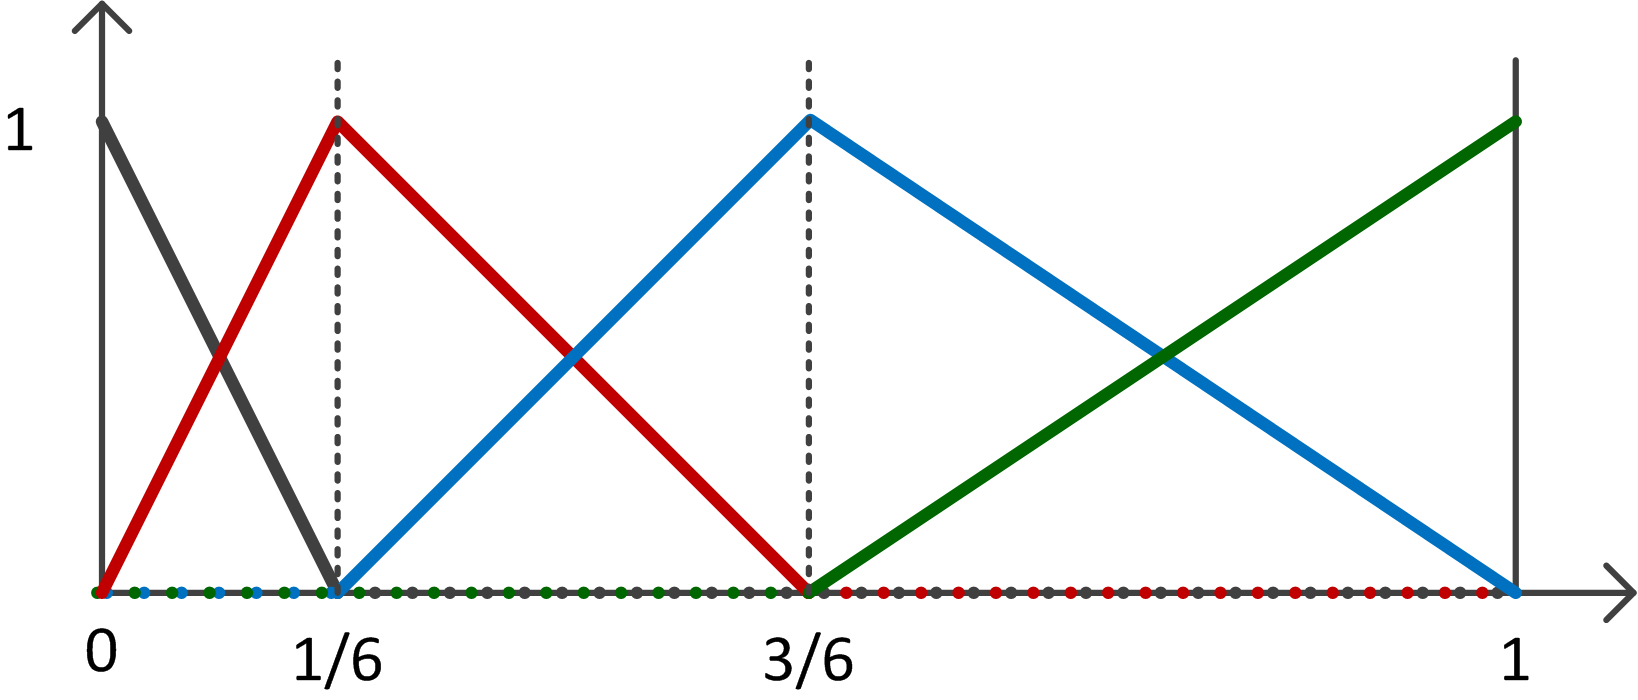
\includegraphics[width=9cm]{Content/02_numerics/FEMHand}
\end{minipage}\\

$R^n\cdot a +r^n=0 \qquad\Rightarrow\qquad
\begin{bmatrix}
	-6 & 6 & 0 & 0\\
	6 & -9 & 3 & 0\\
	0 & 3 & -5 & 2\\
	0 & 0 & 2 & -2\\
\end{bmatrix}\cdot
\begin{bmatrix}
	10\\
	a_1\\
	a_2\\
	20
\end{bmatrix}+
\begin{bmatrix}
	5/3\\
	5\\
	25/3\\
	5
\end{bmatrix}=
\begin{bmatrix}
	0\\
	0\\
	0\\
	0
\end{bmatrix}\qquad\Rightarrow\qquad
\begin{bmatrix}
	6 & -9 & 3 & 0\\
	0 & 3 & -5 & 2\\
\end{bmatrix}\cdot
\begin{bmatrix}
	10\\
	a_1\\
	a_2\\
	20
\end{bmatrix}+
\begin{bmatrix}
	5/3\\
	5\\
	25/3\\
	5
\end{bmatrix}=
\begin{bmatrix}
	0\\
	0\\
	0\\
	0
\end{bmatrix}	
$\\
\\

$\qquad\Rightarrow\qquad
\begin{bmatrix}
	-9 & 3\\
	3 & -5\\
\end{bmatrix}\cdot
\begin{bmatrix}
	a_1\\
	a_2\\
\end{bmatrix}+
\begin{bmatrix}
	6\cdot 10\\
	2\cdot 20\\
\end{bmatrix}+
\begin{bmatrix}
	5\\
	25/3\\
\end{bmatrix}
=0\qquad\Rightarrow\qquad
\begin{bmatrix}
	-9 & 3\\
	3 & -5\\
\end{bmatrix}\cdot
\begin{bmatrix}
	a_1\\
	a_2\\
\end{bmatrix}=
\begin{bmatrix}
	-65\\
	-145/3\\
\end{bmatrix}\qquad\Rightarrow\qquad
\begin{bmatrix}
	a_1\\
	a_2\\
\end{bmatrix}=
\begin{bmatrix}
	235/18\\
	35/2\\
\end{bmatrix}
$\\
\\
$
\qquad\Rightarrow\qquad \tilde{u}(x)=10\cdot v_0(x)+\frac{235}{18} v_1(x)+\frac{35}{2}\cdot v_2(x)+20\cdot v_3(x)=
$




\subsubsection{h-Strategie}

Die Grundidee der h-Strategie ist die Verfeinerung der Auflösung. Mit anderen Worten die Maschenbreite $h$ wird verkleinert. Um den ganzen Bereich dennoch abdecken zu können sind mehr Maschen notwendig.

\subsubsection{p-Strategie}
Bei der p-Strategie bleibt das Netz bestehen. Die Ansatzfunktionen sollen nun durch Polynome höherer Ordnung zusammengesetzt werden, dazu werden neue Knoten und Knotenvariablen eingeführt werden.\\

\textbf{Problemstellung:} $u''(x)+f(x)=0\qquad u(0)=a_0\qquad u(1)=a_6$\\

Die Approximation soll auf dem gleichverteilten Intervallen gelten: $[0,1/3]$,\quad $[1/3,2/3]$,\quad $[2/3,1]$\\

\begin{minipage}{4cm}
	Formfunktionen:\\

	$q_1(x)=(1-x)\cdot(1-2x)$\\
	$q_2(x)=4x\cdot(1-x)$\\
	$q_3(x)=-x\cdot(1-2x)$\\
	
	Elementmatrize: $\boxed{E=\frac{1}{3}
	\begin{bmatrix}
		-7& 8 & -1\\
		8& -16& 8\\
		-1& 8& -7	
	\end{bmatrix}}$\\
\end{minipage}
\hfill
\begin{minipage}{8cm}
	\begin{tabular}{lc|c|c}
		$x\in$&$[0,1/3]$&$[1/3,2/3]$&$[2/3,1]$\\
		\hline
		$v_0=$&$q_1(3x)$&$0$&$0$\\
		$v_1=$&$q_2(3x)$&$0$&$0$\\
		$v_2=$&$q_3(3x)$&$q_1(3x-1)$&$0$\\
		$v_3=$&$0$&$q_2(3x-1)$&$0$\\
		$v_4=$&$0$&$q_3(3x-1)$&$q_1(3x-2)$\\
		$v_5=$&$0$&$0$&$q_2(3x-2)$\\
		$v_6=$&$0$&$0$&$q_3(3x-2)$\\
	\end{tabular}
\end{minipage}
\hfill
\begin{minipage}{6cm}
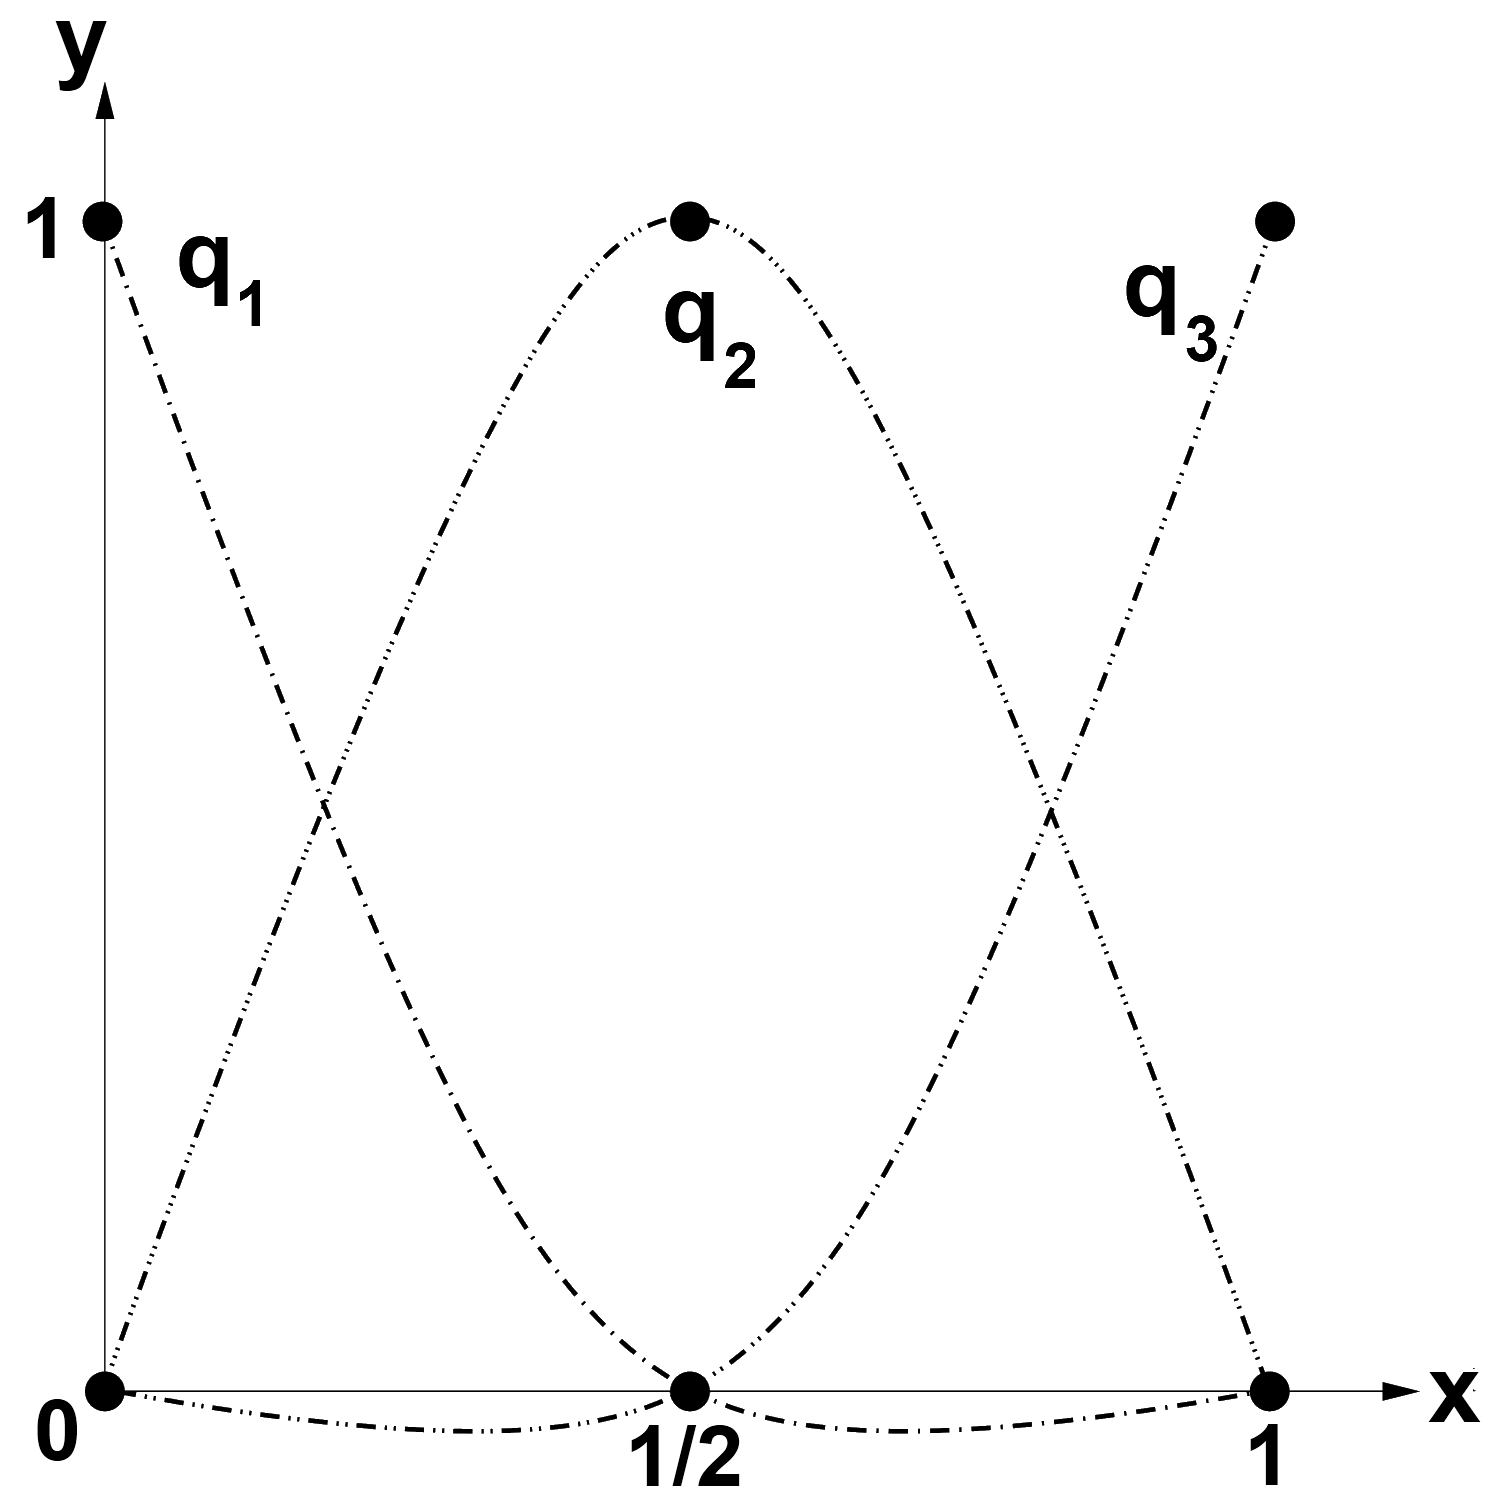
\includegraphics[width=6cm]{Content/02_numerics/FEM2Ord}
\end{minipage}\\

$\underset{\text{Ritzsche Matrize $R^{(8)}$ für } h=1/3}{\underbrace{\begin{bmatrix}
	-7& 8 & -1& 0& 0& 0& 0\\
	 8& -16& 8& 0& 0& 0& 0\\
	-1& 8& -14& 8& -1& 0& 0\\ 
	 0& 0& 8& -16& 8& 0& 0\\
	 0& 0& -1& 8& -14& 8& -1\\ 
	 0& 0& 0& 0& 8& -16& 8\\
	 0& 0& 0& 0& -1& 8& -7	
\end{bmatrix}}}\cdot\begin{bmatrix}
	a_0\\
	a_1\\
	a_2\\
	a_3\\
	a_4\\
	a_5\\
	a_6\\
\end{bmatrix}
+\underset{\text{Ritzscher Vektor $r^{(8)}$ für } h=1/3}{\underbrace{\begin{bmatrix}
	\int\limits_{0}^{1}{f(x)\cdot v_0(x)dx}\\
	\int\limits_{0}^{1}{f(x)\cdot v_1(x)dx}\\
	\int\limits_{0}^{1}{f(x)\cdot v_2(x)dx}\\
	\int\limits_{0}^{1}{f(x)\cdot v_3(x)dx}\\
	\int\limits_{0}^{1}{f(x)\cdot v_4(x)dx}\\
	\int\limits_{0}^{1}{f(x)\cdot v_5(x)dx}\\
	\int\limits_{0}^{1}{f(x)\cdot v_6(x)dx}\\
\end{bmatrix}}}=
\begin{bmatrix}
	0\\
	0\\
	0\\
	0\\
	0\\
	0\\
	0\\
	0\\
\end{bmatrix}
$\\

\textbf{Vorteil der p-Strategie gegenüber der h-Strategie:} Bei beiden Strategien steigt die Dimension der Systemmatrizen an. Es besteht jedoch die berechtigte Hoffnung, dass der Zuwachs der benötigt wird, um eine vergleichbare Genauigkeit zu errreichen, bei der p-Strategie weitaus geringer ist als bei der h-Strategie. 

\subsection{Konformität und Vollständigkeit}
Muss nun die Approximationslösung zweimal ableitbar sein, so gilt der Ansatz des letzten Abschnitt nicht mehr als konform.

Um die einmalige Differenzierbarkeit an den Knoten zu gewährleisten müssen neue Grundfunktionen gefunden werden.\\

$\tilde{u}(x)=a_0v_0(x)+a_1v_1(x)+a_2v_2(x)+a_3v_3(x)+\tilde{a}_0\tilde{v}_0(x)+\tilde{a}_1\tilde{v}_1(x)+\tilde{a}_2\tilde{v}_2(x)+\tilde{a}_3\tilde{v}_3(x)$\\

Zwei Grundfunktionen stellen den richtigen Wert and den Knoten sicher. Zwei weitere Grundfunktionen werden benötigt um die erste Ableitung (Steigung) an den Übergangknoten sicherzustellen, sie sorgen für die Vollständigkeit der Grundfunktionen. (Ohne die zwei weiteren Grundfunktionen wäre an den Übergangsknoten nur eine Steigung von Null möglich.)

\subsection{Hermetische Polynome dritter Ordnung}
Übereinstimmung bis zur 1.Ableitung an den Knotenpunkten\\

\textbf{Problemstellung:} $u''(x)+f(x)=0\qquad u(0)=a_0\qquad u'(0)=\tilde{a}_0 \qquad u(1)=a_3\qquad  u'(1)=\tilde{a}_3$\\

Die Approximation soll auf dem gleichverteilten Intervallen gelten: $[0,1/3]$,\quad $[1/3,2/3]$,\quad $[2/3,1]$\\

\begin{minipage}{4cm}
Formfunktionen:\\
$h_1(x)=2x^3-3x^2+1$\\
$h_2(x)=x^3-2x^2+x$\\
$h_3(x)=-2x^3+3x^2$\\
$h_4(x)=x^3-x^2$
\end{minipage}
\hfill
\begin{minipage}{8cm}
	\begin{tabular}{lc|c|c}
		$x\in$&$[0,1/3]$&$[1/3,2/3]$&$[2/3,1]$\\
		\hline
		$v_0=$&$h_1(3x)$&$0$&$0$\\
		$\tilde{v}_0=$&$\frac 13 h_2(3x)$&$0$&$0$\\
		$v_1=$&$h_3(3x)$&$h_1(3x-1)$&$0$\\
		$\tilde{v}_1=$&$\frac 13 h_4(3x)$&$\frac 13 h_2(3x-1)$&$0$\\
		$v_2=$&$0$&$h_3(3x-1)$&$h_1(3x-2)$\\
		$\tilde{v}_2=$&$0$&$\frac 13 h_4(3x-1)$&$\frac 13 h_2(3x-2)$\\
		$v_3=$&$0$&$0$&$h_3(3x-2)$\\
		$\tilde{v}_3=$&$0$&$0$&$\frac 13 h_2(3x-1)$\\
	\end{tabular}
\end{minipage}
\hfill
\begin{minipage}{6cm}
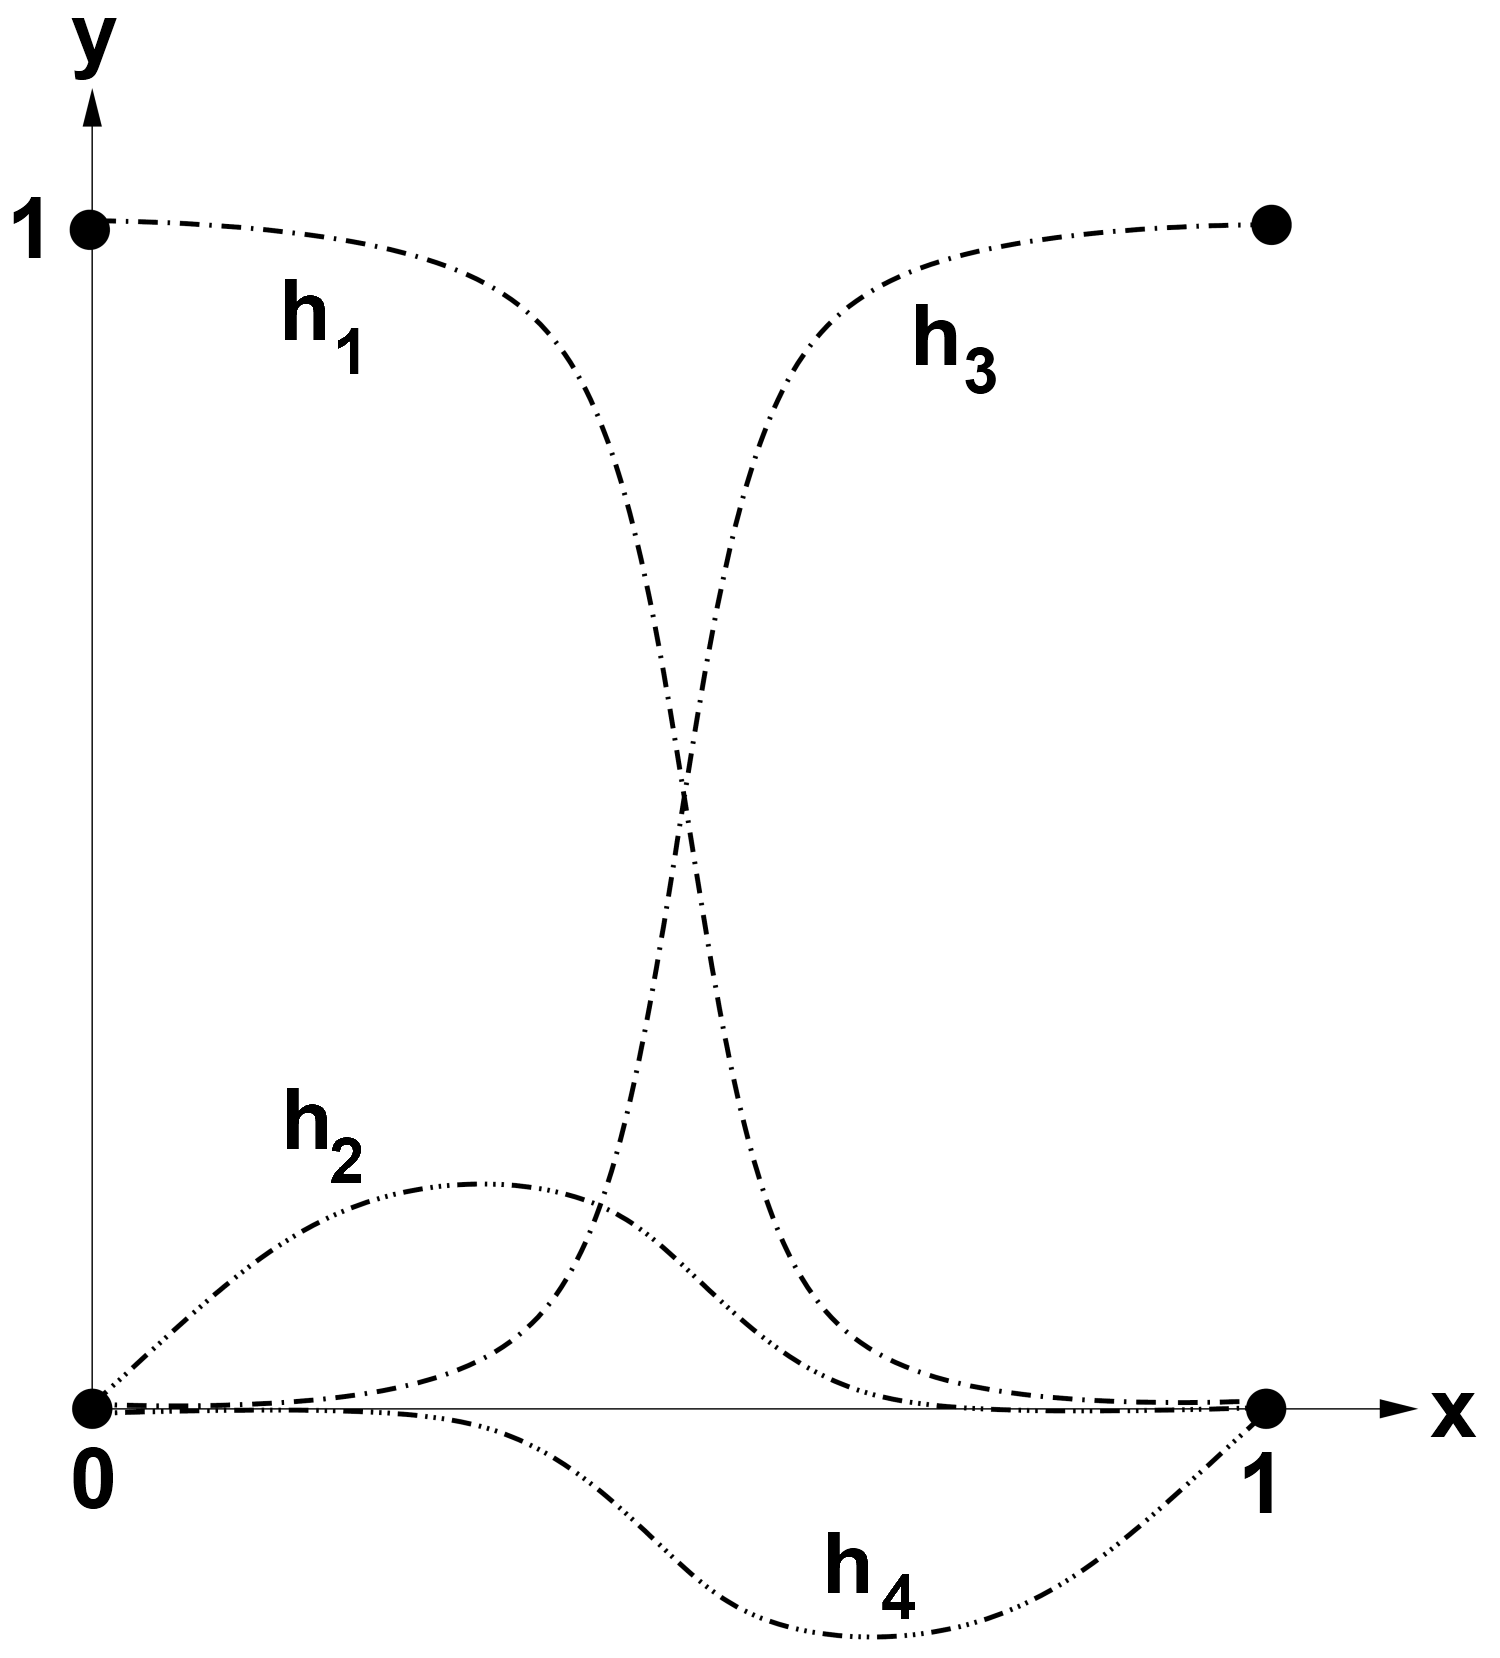
\includegraphics[width=6cm]{Content/02_numerics/FEM3Ord}
\end{minipage}\\
$E=\frac{1}{30}
\begin{bmatrix}
	-36 & -3 & 36 & -3\\
	-3 & -4 & 3 & 1\\
	36 & 3 & -36 & 3\\
	-3 & 1 & 3 & -4\\
\end{bmatrix}\qquad\Rightarrow\qquad
\boxed{M=\frac{1}{30\cdot h}
\begin{bmatrix}
	-36 & -3\cdot h & 36 & -3\cdot h\\
	-3\cdot h & -4\cdot h^2 & 3\cdot h & 1\cdot h^2\\
	36 & 3\cdot h & -36 & 3\cdot h\\
	-3\cdot h & 1\cdot h^2 & 3\cdot h & -4\cdot h^2\\
\end{bmatrix}}$\\
\\


$\underset{\text{Ritzsche Matrize $R^{(8)}$ für } h=1/3}{\underbrace{\frac{3}{30}\begin{bmatrix}
	-36 & -1 & 36 & -1 & 0  & 0  & 0  & 0 \\
	-1  & -4/9  & 1  & 1/9  & 0  & 0  & 0  & 0\\
	36  & 1  & -72  & 0  & 36  & -1  & 0  & 0\\
	-1  & 1/9  & 0  & -8/9  & 1  & 1/9  & 0  & 0\\
	0  & 0  & 36  & 1  & -72  & 0  & 36  & -1\\
	0  & 0  & -1  & 1/9  & 0  & -8/9  & 1  & 1/9\\
	0  & 0  & 0  & 0  & 36  & 1  & -36  & 1\\
	0  & 0  & 0  & 0  & -1  & 1/9  & 1  & -4/9\\
\end{bmatrix}}}\cdot\begin{bmatrix}
	a_0\\
	\tilde{a}_0\\
	a_1\\
	\tilde{a}_1\\
	a_2\\
	\tilde{a}_2\\
	a_3\\
	\tilde{a}_3\\
\end{bmatrix}
+\underset{\text{Ritzscher Vektor $r^{(8)}$ für } h=1/3}{\underbrace{\begin{bmatrix}
	\int\limits_{0}^{1}{f(x)\cdot v_0(x)dx}\\
	\int\limits_{0}^{1}{f(x)\cdot \tilde{v}_0(x)dx}\\
	\int\limits_{0}^{1}{f(x)\cdot v_1(x)dx}\\
	\int\limits_{0}^{1}{f(x)\cdot \tilde{v}_1(x)dx}\\
	\int\limits_{0}^{1}{f(x)\cdot v_2(x)dx}\\
	\int\limits_{0}^{1}{f(x)\cdot \tilde{v}_2(x)dx}\\
	\int\limits_{0}^{1}{f(x)\cdot v_3(x)dx}\\
	\int\limits_{0}^{1}{f(x)\cdot \tilde{v}_3(x)dx}\\
\end{bmatrix}}}=
\begin{bmatrix}
	0\\
	0\\
	0\\
	0\\
	0\\
	0\\
	0\\
	0\\
\end{bmatrix}
$\\







%\subsection{FEM für parabolische PDEs}

\newpage
\section{Fourierreihe}
  	Komplex: $$\boxed{f(t) = \sum\limits_{k = -\infty}^{\infty} c_k \cdot e^{j k
  	\omega_f t}}= \sum\limits_{k = 0}^{\infty} \left(c_k \cdot e^{j k \omega_f
  	t} + \overline{c_k} \cdot e^{-j k \omega_f t}\right) \quad
  	\boxed{c_k=\overline{c_{-k}}=\frac{1}{T}\int_0^T{f(t)\cdot
	e^{-jk\omega_f t}dt}}$$
	
	\vspace{0.5cm}
	
  	Reell: $$\boxed{f(t) = \frac{a_0}{2} + \sum\limits_{k=1}^{\infty} \left[a_k
  	\cos(k \omega_f t) + b_k \sin(k \omega_f t)\right]}=\frac{A_0}{2} +
  	\sum\limits_{k=1}^{\infty} A_k \cos(k \omega_f t + \varphi_k) \quad k\in
  	\mathbb{Z}$$	
	
	$$\boxed{a_0 =
	\frac{2}{T}\int\limits_0^{T} f(t)dt, \quad a_k = \frac{2}{T}\int\limits_0^{T} f(t)\cos(k \omega_f t) dt, \quad b_k =
	\frac{2}{T}\int\limits_0^{T} f(t)\sin(k \omega_f t) dt} \quad
	\boxed{\omega_f=\frac{2 \pi}{T}=2 \pi f}$$
	
	\vspace{0.5cm}

	$a_0$, $c_0$, $A_0$ sind \textit{Konstanten}, $\omega_f$ ist die
	\textit{Grundkreisfrequenz}, $a_k$ und $b_k$ sind die \textit{reellen
	Koeffizienten}, $c_k$ ist der \textit{komplexe Koeffizient}, $A_k$ ist die
	\textit{Amplitude} und $\varphi_k$ ist die \textit{Phase}.\\
	\fbox{
	\begin{tabular}{p{9cm}p{9cm}}
		$a_k = c_k + \bar{c_k} = 2\Real(c_k) = A_k \cos(\varphi_k)$ &
		$b_k = j(c_k + \bar{c_k}) = -2\Imag(c_k) = -A_k \sin(\varphi_k)$ \\ \\
		$c_k = \frac{a_k-jb_k}{2} = \frac{A_k}{2} e^{j\varphi_k}$ &
		$c_{-k} = \overline{c_k} = \frac{a_k+jb_k}{2} = \frac{A_k}{2} e^{-j\varphi_k}$ \\ \\
		$A_k = 2|c_k| = \sqrt{a_k^2+b_k^2}$
	\end{tabular}}\\

	\textbf{Berechnung von $\varphi_k$ aus $a_k$ und $b_k$}\\
	\begin{tabular}{|p{4cm}p{4cm}|p{3cm}p{3.5cm}|}
		\hline
		$a_k> 0:$ & $\varphi_k = -\arctan(\frac{b_k}{a_k})$ &
		$a_k<0:$ &	$\varphi_k = -\arctan(\frac{b_k}{a_k}) + \pi$\\
		\hline
		$a_k = 0; b_k > 0:$ &	$\varphi_k = -\frac{\pi}{2}$ &
		$a_k = 0; b_k < 0:$ &	$\varphi_k = \frac{\pi}{2}$\\
		\hline
		$a_k = b_k = 0:$ &	$\varphi_k = \text{nicht definiert}$ & & $\varphi_k =
		arg(c_k)$\\
		\hline
	\end{tabular}

	\subsection{Symmetrie}
		\begin{tabular}{|p{4.3cm}|p{4.3cm}|p{4.4cm}|p{4.4cm}|}
         	\hline
        	\textbf{gerade Funktion} & \textbf{ungerade Funktion} &
        	\textbf{Halbperiode 1} & \textbf{Halbperiode 2}\\
        	\hline
        	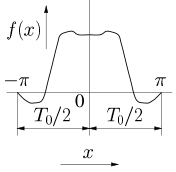
\includegraphics[width=3cm]{Content/Transformationen/gerade_funktion.png}&
        	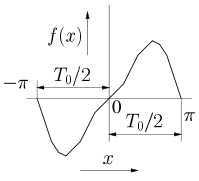
\includegraphics[width=3cm]{Content/Transformationen/ungerade_funktion.png}&   
 			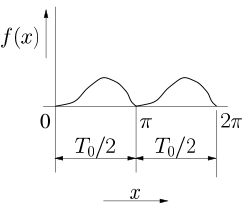
\includegraphics[width=3cm]{Content/Transformationen/halbperiode_1.png}&   
			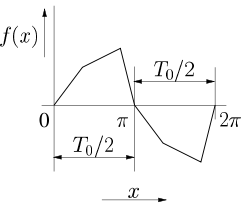
\includegraphics[width=3cm]{Content/Transformationen/halbperiode_2.png}\\
			\hline & & & \\			
   			$f(-t)=f(t)$ & $f(-t)=-f(t)$ & $f(t)=f(t+\pi)$ & $f(t)=-f(t+\pi)$\\
   			$b_k=0$ & $a_k=0$ & $a_{2k+1}=0$ & $a_{2k}=0$\\
   			$a_k = \frac{4}{T} \int\limits_0^{\frac{T}{2}} f(t) \cdot \cos(k \omega_f
   			t) dt$ &
   			$b_k =  \frac{4}{T} \int\limits_0^{\frac{T}{2}} f(t) \cdot
			\sin(k \omega_f t) dt$ &
			$b_{2k+1}=0$ & $b_{2k}=0$\\
			\hline
      	\end{tabular} 
     	
   \subsection{Spektern}
   	\begin{tabular}{p{6cm} p{6cm} p{6cm}}
   		Kosinus- Sinusamplitudenspektrum & 
   		Einseitiges Amplituden-/ Phasenspek. &
   		Zweiseitges Amplituden-/ Phasenspek. \\
   		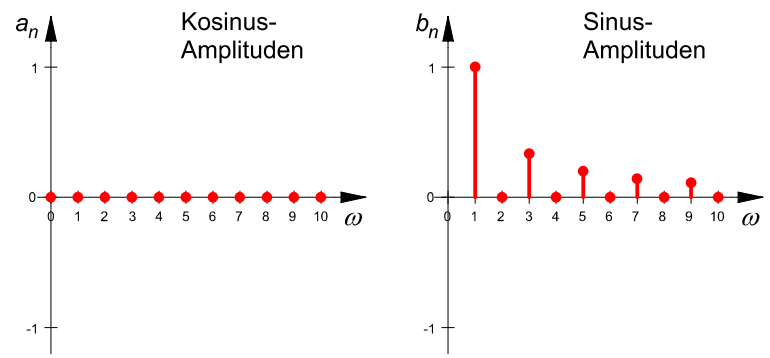
\includegraphics[width=5cm]{Content/Transformationen/cosSinSpectr.png} &
   		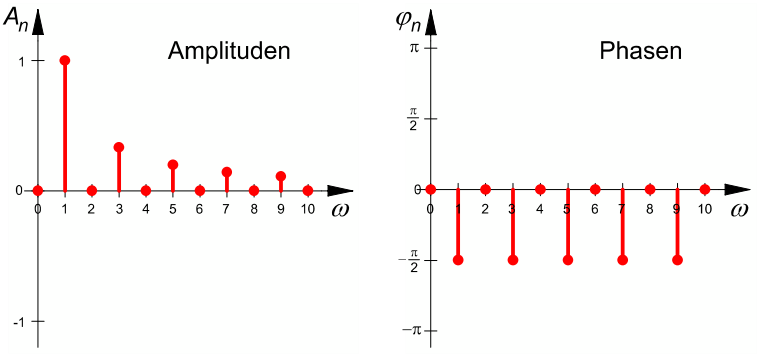
\includegraphics[width=5cm]{Content/Transformationen/EinseitigSpectr.png} &
   		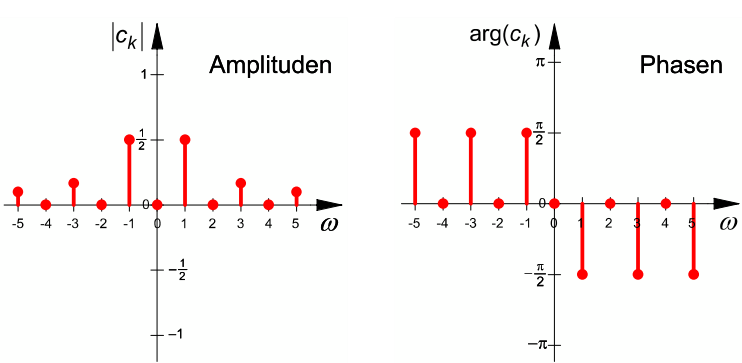
\includegraphics[width=5cm]{Content/Transformationen/ZweiseitigSpectr.png}
   	\end{tabular}
   	Das einseitige und zweiseitige Spektrum unterscheiden sich nur im
  	Amplitudendiagramm. Das Phasendiagramm f"ur positive $k$ ist identisch. Die
  	Amplidudenwerte sind h"alftig auf die pos. und neg. $k$ verteilt.
 
\section{Fourier Transform}
	$$\boxed{f(t) =  \frac{1}{2\pi}\int\limits_{-\infty}^{\infty}
	F(\omega)e^{j\omega t}d\omega}=\frac{1}{2
	\pi}\int\limits_{-\infty}^{\infty}[R(\omega) \cos(\omega t) + X(\omega)
	\sin(\omega t)]d\omega + \frac{j}{2 \pi}\int \limits_{-
	\infty}^{\infty}[R(\omega) \sin(\omega t)- X(\omega) \cos(\omega t)]d\omega$$

	$$\boxed{F(\omega) = \int\limits_{-\infty}^{\infty} f(t)e^{-j\omega t}dt}
	= R(\omega) - j X(\omega) \quad R(\omega) = \int\limits_{-\infty}^{\infty}
	f(t)\cos(\omega t)dt \quad \mbox{ and } \quad X(\omega)=
	\int\limits_{-\infty}^{\infty}f(t)\sin(\omega t)dt$$
	\begin{tabular}{lllll}
	 $ \sigma(t) \FT \frac{1}{j\omega}+\pi \cdot \delta(\omega) $ & \hspace{6mm} &
	 $ \frac{1}{\pi \cdot t} \FT -j \cdot sgn(\omega) $ & \hspace{6mm} &  \\
	 $ 1 \FT 2\pi \cdot \delta(t) \underbrace{\longleftrightarrow}_{Careful}
	 \delta(\omega) \FT 1 $ & & $ sgn(t) \FT \frac{2}{j\omega} $
	\end{tabular}

	\subsection{Properties}
		Fourier integral exists if $\int\limits_{-\infty}^{\infty}|f(t)| dt <
	\infty$\\
		\renewcommand{\arraystretch}{2}
		\begin{tabular}{|p{8cm}|l c l|}
        	\hline
        	Linearity &
        	$\alpha\cdot f(t) + \beta\cdot g(t)$ & $\FT$ & $\alpha\cdot F(\omega) +
        	\beta\cdot G(\omega)$\\
        	\hline
			Time reversal (reflection at the y-axis) &
			$f(-t)$ & $\FT$ & $F(-\omega) = F^*(\omega)$ \\
			\hline
  			Similarity &
  			$f(\alpha t)$ & $\FT$ & $\frac{1}{|\alpha|}F \left( \frac{\omega}{\alpha} \right)
  			\quad\alpha \in\mathbb{R}\setminus \{0\}$\\
  			\hline
  			Time-domain shift &
  			$f(t\pm t_0)$ & $\FT$ & $F(\omega)e^{\pm j\omega t_0}$\\
  			\hline
			Frequency-domain shift &
			$f(t)e^{\pm j\omega_0 t}$ & $\FT$ & $F(\omega\mp\omega_0)$\\
			\hline
			Time-domain differentiation &
			$\frac{\partial^n f(t)}{\partial t^n}$ & $\FT$ & $(j\omega)^n F(\omega)$\\
			\hline
			Time-domain integration &
			$\int\limits_{-\infty}^{t}f(\tau)d\tau $ & $\FT$ &
			$\frac{F(\omega)}{j\omega}+\pi F(0)\delta(\omega)$\\
			\hline
			Frequency-domain differentiation &
			$t^n f(t)$ & $\FT$ & $j^n \frac{\partial F(\omega)}{\partial \omega^n}$\\
			\hline
			Time-domain convolution &
			$f(t) \ast g(t)$ & $\FT$ & $F(\omega) \cdot G(\omega)$\\
			\hline
			Frequency-domain convolution &
			$f(t) \cdot g(t)$ & $\FT$ & $\frac{1}{2\pi}F(\omega) \ast G(j\omega)$\\
			\hline
			Exchange theorem (Duality) &
			$f(t)$ & $\FT$ & $F(\omega)\nonumber$ \\
 			& $F(t)$ & $\FT$ & $2\pi \cdot f(-\omega)$\\
 			\hline
 			Modulation &
 			$\cos(\alpha t) \cdot f(t)$ & $\FT$ & $\frac{1}{2}\cdot
 			\left[F(\omega-\alpha) + F(\omega+\alpha)\right]$\\
 			& $\sin(\alpha t) \cdot f(t)$ & $\FT$ & $\frac{1}{2j}\cdot \left[
 			F(\omega-\alpha) - F(\omega+\alpha)\right]$\\
 			\hline
        	Parseval's Theorem &
 			$\int\limits_{-\infty}^{\infty}f(t)g^{\ast}(t)dt $ & $=$ & $ \frac{1}{2\pi}
  			\int\limits_{-\infty}^{\infty}F(\omega)G^{\ast}(\omega)d\omega$\\
  			\hline
  			Bessel's Theorem &
  			$\int\limits_{-\infty}^{\infty}|f(t)|^2 dt $ & $=$ & $ \frac{1}{2\pi}
  			\int\limits_{-\infty}^{\infty}|F(\omega)|^2 d\omega$\\
  			\hline
			Initial values &
			$f(0)=\frac{1}{2\pi}\int\limits_{-\infty}^{\infty}F(\omega)d\omega
			$ && $ F(0)=\int\limits_{-\infty}^{\infty}f(t)dt$\\
			\hline
			Infinite sequence of $\delta$-impulses &
			$\sum\limits_{n=-\infty}^{\infty} \delta(t-n\cdot t_0)$ & $\FT$ &
			$\sum\limits_{n=-\infty}^{\infty}
			\frac{2\pi}{t_0}\delta(\omega-n\cdot \frac{2\pi}{t_0})$\\
			\hline
        \end{tabular}
		\renewcommand{\arraystretch}{1}

\section{Laplace Transformation}
	$$\boxed{F(s)=\int\limits_0^\infty f(t)e^{-st}dt} \qquad s=\sigma +j\omega$$\\
	- Definitionsbereich nur für \textbf{kausale} Systeme $\boxed{t\geq 0}$\\
	- Integrierbar über das Intervall $(0,\infty)$\\
	- Wachstum kleiner als der von eienr Exponentialfunktion $\boxed{\sigma > 0}$\\
	- $\sigma$ ist der Dämpfungsfaktor: $e^{-s}=e^{-\sigma} \cdot e^{-j\omega}$ \\
	- Fourier-Transformierte $F(\omega)$ kann durch die
	Laplace-Transformation $F(s)$ ausgedrückt werden.  \\
	- Fourier $\longleftrightarrow$ Laplace Umwandlungen nur wenn Polstelle
	($\sigma > 0$) dh. links von $j\omega$ Achse und kausal!\\
	- $f(0+)$: Entspricht der Anfangsbedingung zum Zeitpunkt > 0 (kausal).
  
 	\subsection{Eigenschaften}
 	    \label{sec:Laplace Umwandulungen}
  		\renewcommand{\arraystretch}{2}
		\begin{tabular}{|l|l c p{5.5cm}|}
        	\hline
        	Linearität & 
 			$\alpha\cdot f(t) + \beta\cdot g(t)$ & $\FT$ & $\alpha\cdot F(s) +
 			\beta\cdot G(s)$ \\
 			\hline
 			Verschiebung im Zeitbereich &
 			$f(t\pm t_0) $ & $\FT$ & $ F(s)e^{\pm t_0 s}$ \\
 			\hline
 			Dämpfung (Verschiebung im Frequenzbereich) &
 			$f(t)e^{\mp\alpha t}$ & $\FT$ & $F(s\pm\alpha)$ \\
 			\hline
 			"Ahnlichkeit&
 			$f(\alpha t)$ & $\FT$ & $\frac{1}{\alpha}F \left (\frac{s}{\alpha} \right )
 			\quad 0 <\alpha \in\mathbb{R}$ \\
 			\hline
 			Faltung im Zeitbereich &
 			$f(t) \ast g(t)$ & $\FT$ &
 			$F(s) \cdot G(s)$\\
 			\hline 			
 			Faltung im Frequenzbereich &
 			$f(t) \cdot g(t)$ & $\FT$ & $\frac{1}{2 \pi j} F(s) \ast G(s)$ \\
 			\hline
 			Differentiation im Zeitbereich &
 			$f'(t)$ & $\FT$ & $sF(s) - f(0+)$ \\ 
 			&
 			$f''(t)$ & $\FT$ & $s^2 F(s) - sf(0+) - f'(0+)$\\ 
 			&
 			$f^{(n)}(t)$ & $\FT$ & $s^nF(s) - s^{n-1}f(0+) - s^{n-2} f'(0+) - \ldots
 			-s f^{(n-2)}(0+) - f^{(n-1)}(0+)$ \\
 			\hline
 			Diffrentation im Frequenzbereich &
 			$(-t)^n f(t)$ & $\FT$ & $F^{(n)}(s)$ \\
 			\hline
 			Integration &
 			$\int\limits_0^t f(\tau)d\tau$ & $\FT$ & $\frac{F(s)}{s}$ \\
 			\hline
 			Anfangswert &
 			$\lim_{t\rightarrow 0} f(t)$ muss exist. & $=$ & $\lim_{s\rightarrow
 			\infty} sF(s)$ \\
 			\hline
 			Endwert &
 			$\lim_{t\rightarrow \infty} f(t)$ muss exist. & $=$ & 
 			$\lim_{s\rightarrow 0} sF(s)$ \\
 			\hline
       	\end{tabular}
		\renewcommand{\arraystretch}{1}
		
		\subsection{Von Laplace zu Fourier}
			$s \rightarrow j\omega$ \hspace{0.5cm}
			Dies kann nur gemacht werden wenn Polstelle ($\sigma > 0$) links von
			$j\omega$-Achse ist und das System kausal ist.
			
		\subsection{Rücktransformation (Komplexe Integration)}
			$$f(t)=\int\limits_{x-j\infty}^{x+j\infty}F(s) \cdot e^{st} \cdot ds$$
			
		\subsection{Vorgehen Rücktransformation}
		\begin{tabular}{ll}
  			1. Ansatz & Versuchen Zähler Gleichnamig mit Nenner machen un danach
  			kürzen (Korrekturen!) \\
  			2. Ansatz & Partitialbruchzerlegung
		\end{tabular}
			
		\newpage
		
		\subsection{Rücktransformation über Tabelle}
			\begin{center}
				$\sigma$ = Step function. When $1$ is transformed, $\sigma$ should be taken (so in the frequency domain, it is $\frac{1}{s}$).
\let\DS=\displaystyle
\renewcommand{\arraystretch}{2.5}
{ \[
\begin{array}{|@{\hspace{1cm}}c@{\hspace{1cm}}c@{\hspace{1cm}}c@{\hspace{1cm}}||c@{\hspace{1cm}}c@{\hspace{1cm}}c@{\hspace{1cm}}c@{\hspace{1cm}}|}
\hline
\sigma(t) & \FT & \DS\frac{1}{s} &&\sigma(t)\cdot t^2\cdot e^{\,\alpha\,t} & \FT & \DS\frac{2}{(s-\alpha)^3} \\
\hline
\sigma(t)\cdot t & \FT & \DS\frac{1}{s^2} &&\sigma(t)\cdot t^n\cdot e^{\,\alpha\,t} & \FT & \DS\frac{n!}{(s-\alpha)^{n+1}} \\
\hline
\sigma(t)\cdot t^2 & \FT & \DS\frac{2}{s^3} &&\sigma(t)\cdot\sin\,(\omega\,t) & \FT & \DS\frac{\omega}{s^2+\omega^2} \\
\hline
\sigma(t)\cdot t^n & \FT & \DS\frac{n!}{s^{n+1}} &&\sigma(t)\cdot\cos\,(\omega\,t) & \FT & \DS\frac{s}{s^2+\omega^2} \\
\hline
\sigma(t)\cdot e^{\,\alpha\,t} & \FT & \DS\frac{1}{s-\alpha} &&\delta(t) & \FT & 1(s) \\
\hline
\sigma(t)\cdot t\cdot e^{\,\alpha\,t} & \FT & \DS\frac{1}{(s-\alpha)^2} &&\delta(t-a) & \FT & e^{-a\,s} \\
\hline
\end{array} \] }

			\end{center}
			\vfill
		
				
\section{Mathe Grundlagen}	

	\subsection{Partialbruchzerlegung}
		
\[f(x)=\frac{x^2+20x+149}{x^3+4x^2-11x-30} \Rightarrow \; \begin{array}{l}\text{Factorize denominator using}\\
	\text{Horner's scheme, binomial, etc.}\end{array} \Rightarrow
	x^{3}+4x^{2}-11x-30=(x+2)(x^{2}+2x-15)=(x+2)(x+5)(x-3)\] Approach:
	\[f(x)=\frac{x^2+20x+149}{x^3+4x^2-11x-30}=\frac{A}{x-3} + \frac{B}{x+2} + \frac{C}{x+5}=
	\frac{A(x+2)(x+5)+B(x-3)(x+5)+C(x-3)(x+2)}{(x-3)(x+2)(x+5)}\]
	Set up a system of equations with arbitrary values of $x_i$ (preferably choose poles or 0,1,-1):
	\[\begin{array}{l}x_1=3:\;-9+60+149=A\cdot5\cdot8\;\;\;\Rightarrow A=5\\
	x_2=-2:\;-4-40+149=B(-5)\cdot3\; \Rightarrow B=-7\\
	x_3=-5:\;-25-100+149=C(-8)(-3) \Rightarrow C=1 \end{array} \Rightarrow
	f(x)=\frac{5}{x-3}-\frac{7}{x+2}+\frac{1}{x+5}\] Additional approaches for other types of terms:
	\[f(x)=\frac{5x^2-37x+54}{x^3-6x^2+9x}=\frac{A}{x}+\frac{B}{x-3}+\frac{C}{(x-3)^2}=\frac{A(x-3)^2+Bx(x-3)+Cx}{x(x-3)^2}\]
	\[f(x)=\frac{1.5x}{x^3-6x^2+12x-8}=\frac{A}{x-2}+\frac{B}{(x-2)^2}+\frac{C}{(x-2)^3}=\frac{A(x-2)^2+B(x-2)+C}{(x-2)^3}\]
	\[f(x)=\frac{x^2-1}{x^3+2x^2-2x-12}=\frac{A}{x-2}+\frac{Bx+C}{x^2+4x+6}=\frac{A(x^2+4x+6)+(Bx+C)(x-2)}{(x-2)(x^2+4x+6)}\]

\subsubsection{Horner's Scheme}
	\begin{minipage}[t]{9cm}
		- Arrows $\Rightarrow$ Multiplication\\
		- Numbers in each column are added\\
		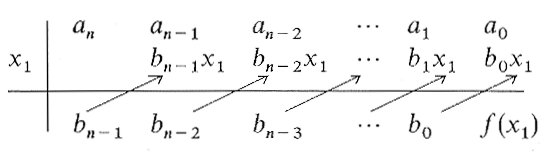
\includegraphics[width=6cm]{Content/04_calculation/hornerschema_1.png}\\
		$x_1 \Rightarrow$ Root (must be guessed!!)\\
		Top row = polynomial to be factored
	\end{minipage}
	\begin{minipage}[t]{9cm}
		\textbf{Example:}\\
		$f(x) = x^3-67x-126$\\
		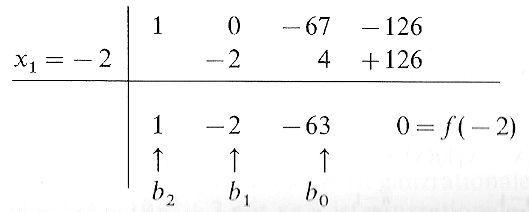
\includegraphics[width=6cm]{Content/04_calculation/hornerschema_2.png}\\
		$\Rightarrow f(x) = (x-x_1)(b_2x^2 + b_1x + b_0) = (x+2)(x^2-2x-63)$
	\end{minipage}

			
	\subsection{Trigonometrie}
			$\sin^2(b)+\cos^2(b)=1 \qquad \tan(b)=\frac{\sin(b)}{\cos(b)} \qquad \cosh(b)^2 - \sinh(b)^2 = 1 \qquad \tanh(b)=\frac{\sinh(b)}{\cosh(b)}$
\subsubsection{Funktionswerte für Winkelargumente}
	\renewcommand{\arraystretch}{1.5}
	\begin{minipage}{5cm}
		\begin{tabular}[c]{ |c|c||c|c|c| }
	    	\hline
			deg & rad & sin & cos & tan\\
			\hline
			0\symbol{23} & 0 & 0 & 1 & 0\\
			\hline
			30\symbol{23} & $\frac{\pi}{6}$ & $\frac{1}{2}$ & $\frac{\sqrt{3}}{2}$ &
			$\frac{\sqrt{3}}{3}$\\
			\hline
			45\symbol{23} & $\frac{\pi}{4}$ & $\frac{\sqrt{2}}{2}$ & $\frac{\sqrt{2}}{2}$
			& 1\\
			\hline
			60\symbol{23} & $\frac{\pi}{3}$ & $\frac{\sqrt{3}}{2}$ & $\frac{1}{2}$ &
			$\sqrt{3}$\\
			\hline			
		\end{tabular}			
	\end{minipage}
	\begin{minipage}{4.3cm}
		\begin{tabular}[c]{ |c|c||c|c|}
	    	\hline
			deg & rad & sin & cos\\
			\hline
			90\symbol{23} & $\frac{\pi}{2}$ & 1 & 0\\
			\hline	
			120\symbol{23} & $\frac{2\pi}{3}$ & $\frac{\sqrt{3}}{2}$ & $-\frac{1}{2}$ \\
			\hline
			135\symbol{23} & $\frac{3\pi}{4}$ & $\frac{\sqrt{2}}{2}$ & $-\frac{\sqrt{2}}{2}$\\
			\hline
			150\symbol{23} & $\frac{5\pi}{6}$ & $\frac{1}{2}$ & $-\frac{\sqrt{3}}{2}$\\
			\hline
		\end{tabular}			
	\end{minipage}
	\begin{minipage}{4.5cm}
		\begin{tabular}[c]{ |c|c||c|c| }
	    	\hline
			deg & rad & sin & cos\\
			\hline
			180\symbol{23} & $\pi$ & 0 & -1\\
			\hline	
			210\symbol{23} & $\frac{7\pi}{6}$ & $-\frac{1}{2}$ & $-\frac{\sqrt{3}}{2}$\\
			\hline
			225\symbol{23} & $\frac{5\pi}{4}$ & $-\frac{\sqrt{2}}{2}$ & $-\frac{\sqrt{2}}{2}$\\
			\hline
			240\symbol{23} & $\frac{4\pi}{3}$ & $-\frac{\sqrt{3}}{2}$ & $-\frac{1}{2}$\\
			\hline
		\end{tabular}			
	\end{minipage}
	\begin{minipage}{4.5cm}
		\begin{tabular}[c]{ |c|c||c|c| }
	    	\hline
			deg & rad & sin & cos\\
			\hline
			270\symbol{23} & $\frac{3\pi}{2}$ & -1 & 0\\
			\hline	
			300\symbol{23} & $\frac{5\pi}{3}$ & $-\frac{\sqrt{3}}{2}$ & $\frac{1}{2}$\\
			\hline
			315\symbol{23} & $\frac{7\pi}{4}$ & $-\frac{\sqrt{2}}{2}$ & $\frac{\sqrt{2}}{2}$\\
			\hline
			330\symbol{23} & $\frac{11\pi}{6}$ & $-\frac{1}{2}$ & $\frac{\sqrt{3}}{2}$\\
			\hline
		\end{tabular}			
	\end{minipage}
	\renewcommand{\arraystretch}{1}
	
\subsubsection{Quadrantenbeziehungen}
	\begin{tabbing}
    	xxxxxxxxxxxxxxxxxxxxxxxxxxxxxxxxxx \= \kill
	  	$\sin(-a)=-\sin(a)$ \> $\cos(-a)=\cos(a)$\\
		$\sin(\pi - a)=\sin(a)$ \> $\cos(\pi - a)=-\cos(a)$\\
		$\sin(\pi + a)=-\sin(a)$ \> $\cos(\pi +a)=-\cos(a)$\\
		$\sin\left(\frac{\pi}{2}-a \right)=\sin\left(\frac{\pi}{2}+a \right)=\cos(a)$ \>
		$\cos\left(\frac{\pi}{2}-a \right)=-\cos\left(\frac{\pi}{2}+a \right)=\sin(a)$  
    \end{tabbing}

	\textbf{Additionstheoreme}
		$\sin(a \pm b)=\sin(a) \cdot \cos(b) \pm \cos(a) \cdot \sin(b) \qquad
		\cos(a \pm b)=\cos(a) \cdot \cos(b) \mp \sin(a) \cdot \sin(b)$\\ 
		$\tan(a \pm b)=\dfrac{\tan(a) \pm \tan(b)}{1 \mp \tan(a) \cdot \tan(b)}$
		
	\subsubsection{Doppel- und Halbwinkel}	
		\begin{tabular}{ll}
			$\sin(2a)=2\sin(a)\cos(a)$ &
			$\cos(2a)=\cos^2(a)-\sin^2(a)=2\cos^2(a)-1=1-2\sin^2(a)$\\
			$\cos^2 \left(\frac{a}{2}\right)=\frac{1+\cos(a)}{2}$ &
			$\sin^2 \left(\dfrac{a}{2}\right)=\frac{1-\cos(a)}{2}$
		\end{tabular}\\
		
	\begin{minipage}[t]{9.5cm}	
		\subsubsection{Produkte}
			$\sin(a)\sin(b)=\frac{1}{2}(\cos(a-b)-\cos(a+b))$\\
			$\cos(a)\cos(b)=\frac{1}{2}(\cos(a-b)+\cos(a+b))$\\
			$\sin(a)\cos(b)=\frac{1}{2}(\sin(a-b)+\sin(a+b))$
		\subsubsection{Hyperbolic}
			$\sinh(z) = \frac{1}{2} \left( e^z - e^{-z} \right) \qquad \cosh(z) =
			\frac{1}{2} \left( e^z + e^{-z} \right) $
	\end{minipage}
	\hfill
	\begin{minipage}[t]{9.5cm}		
		\subsubsection{Summe und Differenz}
			$\sin(a)+\sin(b)=2 \cdot \sin \left(\frac{a+b}{2}\right) \cdot
			\cos\left(\frac{a-b}{2}\right)$\\
			$\sin(a)-\sin(b)=2 \cdot \sin \left(\frac{a-b}{2}\right) \cdot
			\cos\left(\frac{a+b}{2}\right)$\\
			$\cos(a)+\cos(b)=2 \cdot \cos \left(\frac{a+b}{2}\right) \cdot
			\cos\left(\frac{a-b}{2}\right)$\\
			$\cos(a)-\cos(b)=-2 \cdot \sin \left(\frac{a+b}{2}\right) \cdot
			\sin\left(\frac{a-b}{2}\right)$\\
			$\tan(a) \pm \tan(b)=\dfrac{\sin(a \pm b)}{\cos(a)\cos(b)}$
	\end{minipage}	
	
		
	\subsubsection{Euler}
	$sin(z)=\frac{e^{jz}-e^{-jz}}{2j} \hspace{2cm}
    cos(z)=\frac{e^{jz}+e^{-jz}}{2} \hspace{2cm}
    e^{j\varphi}=cjs(\varphi)=cos(\varphi)+j sin(\varphi)$
    
    \subsubsection{Komplex}
    \begin{tabular}{lll}
     	Betrag: & $ |z| = \sqrt{Re(z)^2 + Im(z)^2} = \sqrt{z \cdot \bar{z}}$\\ 
     	Konjugiertkomplex: & $z=z_1 + jz_2$ & $\bar{z}=z^*=z_1-jz_2$
     \end{tabular}
	
			
	\subsection{Taylor Polynom}
		$f(x_0+h)=f(x_0) + f'(x_0)h + \frac{f''(x_0)}{2}h^2 + \frac{f'''(x_0)}{3!}h^3 + \ldots + \frac{f^{(n)}(x_0)}{n!}h^n + R_n(x_0, h)$

	\subsection{Integralrechnung}	
	\begin{tabbing}
	     xxxxxxxxxxxxxxxxxxxxxxxxxxxxxxx \= xxx \= xxxxxxxxxxxxxxxxxxxxxxxxxxxxxxxxxxxxxxxxxxxxxxxxxxxxxxx\kill  
	     Integration\>\>$A=\int\limits_{a}^{b}{f(t)dt}=\left[F(t)\right]_a^b=F(b)-F(a)$\\[0.2cm]
	     Linearität\>		  
	   $\qquad\int{f(\alpha x+\beta )dx=\frac{1}{\alpha}\cdot F(\alpha x+
				\beta)+C}$\\[0.2cm]
		   Partielle Integration\>
	   $\qquad\int\limits_a^b{\underset{\Uparrow}{u}'(x)\cdot \underset{\Downarrow}{v}(x)dx}=\biggl[ u(x)\cdot v(x) \biggr]_a^b
	   -\int\limits_a^b{u(x)\cdot v'(x)dx}$\\[0.2cm]
	   Substitution (Rationalisierung)\>
	   $\qquad t=\tan\frac{x}{2}, \qquad dx=\frac{2dt}{1+t^2} \qquad 
	   \sin  x=\frac{2t}{1+t^2} \qquad \cos x=\frac{1-t^2}{1+t^2}
				\quad\int{R(\sin(x)\cos(x))dx}$\\ 
	   Allgemeine Substitution \> \>
				$\int\limits_{a}^{b}{f(x)dx}=\int\limits_{g^{-1}(a)}^{g^{-1}(b)}{f(g(t))\cdot
				g'(t)dt}\qquad t=g^{-1}(x)\qquad  \fbox{x=g(t)}\qquad dx=g'(t)\cdot dt$\\
	   Logarithmische Integration \>\>
	    $ \int{\frac{f'(x)}{f(x)}dx}=\ln|f(x)|+C	\qquad{(f(x)\neq 1)}$\\[0.2cm]
	  Spezielle Form des Integranden \>\>
		 		$\int{f'(x)\cdot (f(x))^{\alpha} dx}= f(x)^{\alpha +1}\cdot
		 		\frac{1}{\alpha+1}+C \qquad{(\alpha \neq -1)}$\\ 
	   Differentiation\>\>
		 		$\int \limits ^{b} _{a} {f'(t)dt}=f(b)-f(a)$\qquad
				$\frac{d}{dx} \int \limits ^{x} _{1} {f(t)dt}=f(x)$
	\end{tabbing}
	%\subsubsection{Einige unbestimmte Integrale}
	%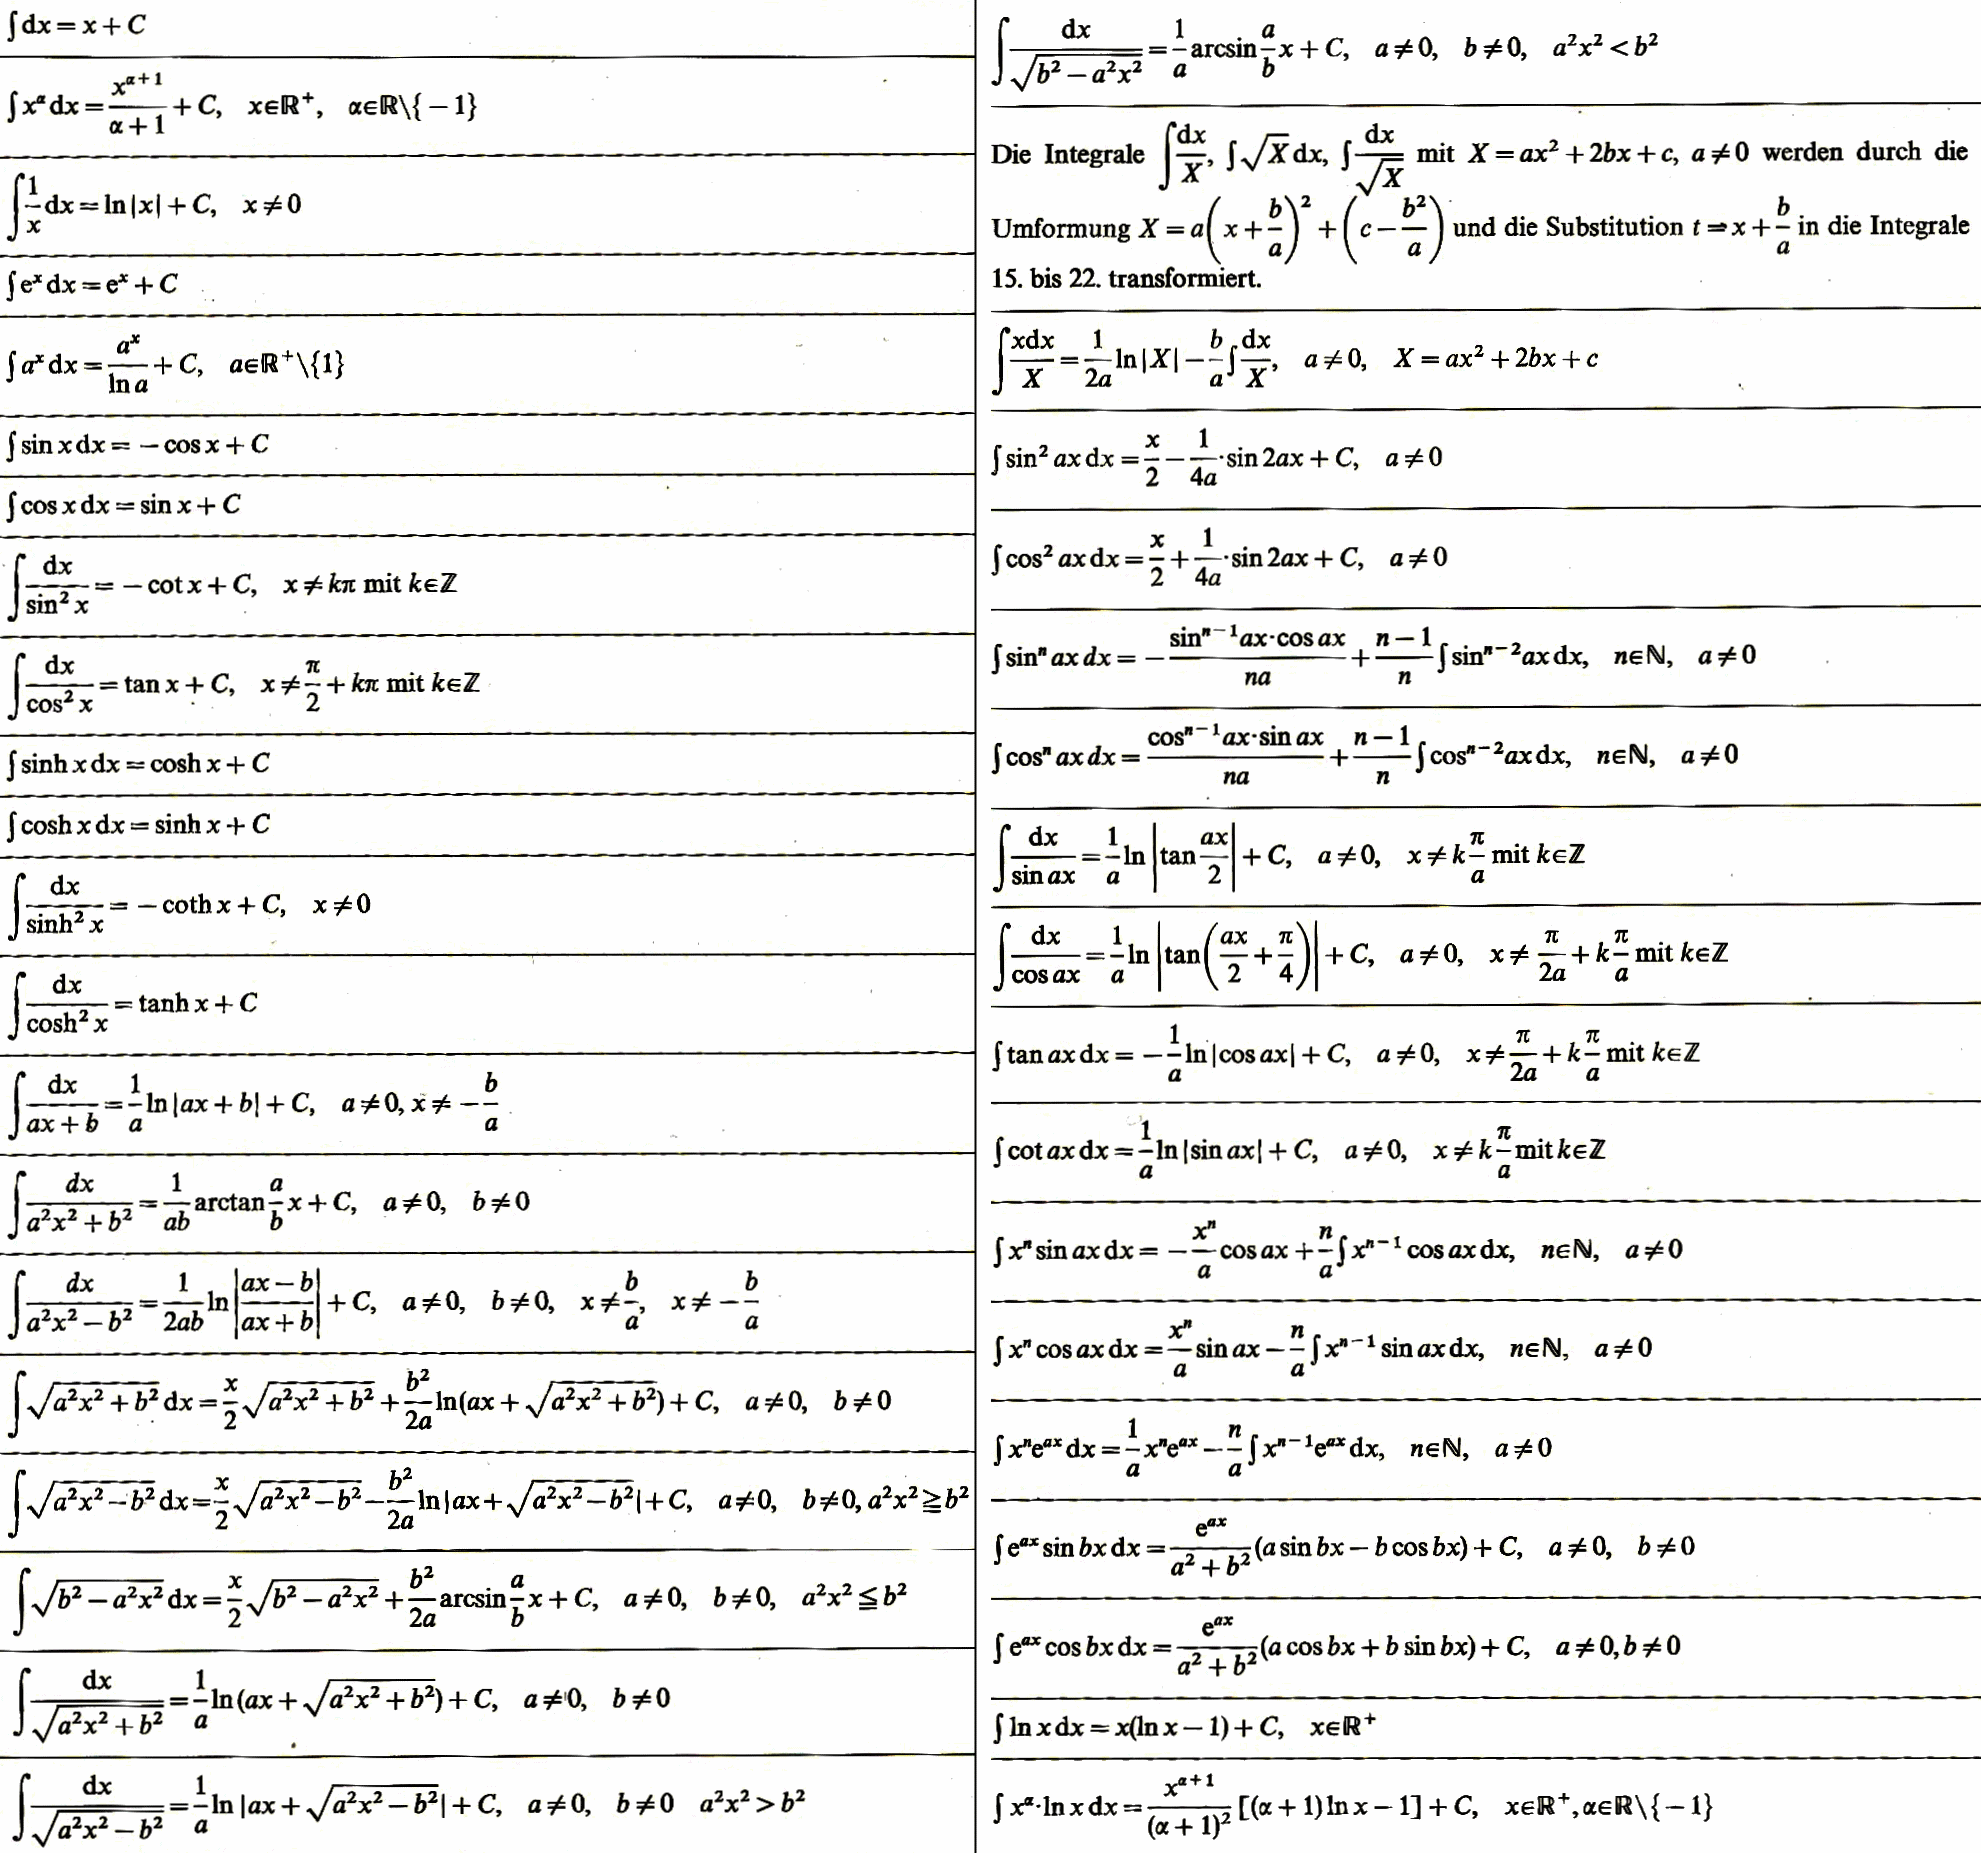
\includegraphics[width=19cm]{Content/04_calculation/integrale.png} 
	
	$\int \mathrm dx = x + C$\\
	$\int x^{\alpha} \mathrm dx = \frac{x^{\alpha + 1}}{\alpha + 1} + C$, $x \in
	\mathbb{R}^+$, $\alpha \in \mathbb{R} \textbackslash \{-1\}$\\
	$\int \frac{1}{x} \mathrm dx = \ln \lvert x \lvert + C$, $x \neq 0$\\
	$\int e^x \mathrm dx = e^x + C$\\
	$\int a^x \mathrm dx = \frac{a^x}{\ln(a)} + C$, $a \in \mathbb{R}^+
	\textbackslash \{1\}$\\
	$\int \sin x \mathrm dx = - \cos x + C$\\
	$\int \cos x \mathrm dx = \sin x + C$\\
	$\int \frac{\mathrm dx}{\sin^2 x} = -\cot(x) + C$, $x \neq k \pi$ mit $k \in
	\mathbb{Z}$\\
	$\int \frac{\mathrm dx}{\cos^2 x} = \tan(x) + C$, $x \neq \frac{\pi}{2} + k \pi$
	mit $k \in \mathbb{Z}$\\
	$\int \sinh(x) \mathrm dx = \cosh(x) + C$\\
	$\int \cosh(x) \mathrm dx = \sinh(x) + C$\\
	$\int \frac{\mathrm dx}{\sinh^2 x} = -\coth(x) + C$, $x \neq 0$\\
	$\int \frac{\mathrm dx}{\cosh^2 x} = \tanh(x) + C$, $x \neq 0$\\
	$\int \frac{\mathrm dx}{ax + b} = \frac{1}{a} \ln \lvert ax + b \lvert + C$, $a
	\neq 0$, $x \neq - \frac{b}{a}$\\
	$\int \frac{\mathrm dx}{a^2x^2 + b^2} = \frac{1}{ab} \arctan(\frac{a}{b} x) +
	C$, $a \neq 0$, $x \neq - \frac{b}{a}$ $x \neq -\frac{b}{a}$\\
	$\int \frac{\mathrm dx}{a^2x^2 - b^2} = \frac{1}{2ab} \ln \lvert \frac{ax -
	b}{ax + b} \lvert + C$, $a \neq 0$, $x \neq - \frac{b}{a}$ $x \neq
	-\frac{b}{a}$\\
	$\int \sqrt{a^2 x^2 + b^2} \mathrm dx = \frac{x}{2} \sqrt{a^2 x^2 + b^2} +
	\frac{b^2}{2a} \ln(ax + \sqrt{a^2 x^2 + b^2}) + C$, $a \neq 0$, $b \neq 0$\\
	$\int \sqrt{a^2 x^2 - b^2} \mathrm dx = \frac{x}{2} \sqrt{a^2 x^2 - b^2} +
	\frac{b^2}{2a} \ln \lvert ax + \sqrt{a^2 x^2 - b^2} \lvert + C$, $a \neq 0$, $b
	\neq 0$, $a^2 x^2 \geq b^2$\\
	$\int \sqrt{b^2 - a^2x^2} \mathrm dx = \frac{x}{2} \sqrt{b^2 - a^2x^2} +
	\frac{b^2}{2a} \arcsin(\frac{a}{b} x) + C)$, $a \neq 0$, $b \neq 0$,
	$a^2 x^2 \geq b^2$\\
	$\int \frac{\mathrm dx}{\sqrt{a^2 x^2 + b^2}} = \frac{1}{a} \ln(ax +
	\sqrt{a^2 x^2 + b^2}) + C$, $a \neq 0$, $b \neq 0$\\
	$\int \frac{\mathrm dx}{\sqrt{a^2 x^2 - b^2}} = \frac{1}{a} \ln(ax +
	\sqrt{a^2 x^2 - b^2}) + C$, $a \neq 0$, $b \neq 0$ $a^2 x^2 > b^2$\\
	$\int \frac{\mathrm dx}{\sqrt{b^2 - a^2 x^2}} = \frac{1}{a}
	\arcsin(\frac{a}{b} x) + C$, $a \neq 0$, $b \neq 0$, $a^2 x^2 < b^2$\\
	Die Integrale $\int \frac{dx}{X}$, $\int \sqrt{X} \; dx$, $\int
	\frac{dx}{\sqrt{X}}$ mit $X = ax^2 + 2bx + c$, $a \neq 0$, werden durch die
	Umformung $X = a \left(x + \frac{b}{a}\right)^2 + \left(c -
	\frac{b^2}{a}\right)$ und die Substitution $t = x + \frac{b}{a}$ in die
	Integrale 15. bis 22. transformiert.\\
	$\int \frac{x \; \mathrm dx}{X}= \frac{1}{2a} \ln \lvert X \lvert - \frac{b}{a}
	\int \frac{dx}{X}$, $a \neq 0$, $X = ax^2 + 2bx + c$\\
	$\int \sin^2(ax) \; \mathrm dx = \frac{x}{2} - \frac{1}{4a} \cdot \sin(2ax) +
	C$, $a \neq 0$\\
	$\int \cos^2(ax) \; \mathrm dx = \frac{x}{2} + \frac{1}{4a} \cdot \sin(2ax) +
	C$, $a \neq 0$\\
	$\int \sin^n(ax) \; \mathrm dx = \frac{\sin^{n-1}(ax) \cdot \cos(ax)}{na} +
	\frac{n-1}{n} \int \sin^{n-2}(ax) \mathrm dx$, $n \in \mathbb N$, $a \neq 0$\\
	$\int \cos^n(ax) \; \mathrm dx = \frac{cos^{n-1}(ax) \cdot \sin(ax)}{na} +
	\frac{n-1}{n} \int \cos^{n-2}(ax) \mathrm dx$, $n \in \mathbb N$, $a \neq 0$\\
	$\int \frac{dx}{\sin (ax)} = \frac{1}{a} \ln \lvert \tan(\frac{ax}{2}) \lvert +
	C$, $a \neq 0$, $x \neq k \frac{\pi}{a}$ mit $k \in \mathbb Z$\\
	$\int \frac{dx}{cos (ax)} = \frac{1}{a} \ln \lvert \tan(\frac{ax}{2} +
	\frac{\pi}{4}) \lvert + C$, $a \neq 0$, $x \neq \frac{\pi}{2a} + k
	\frac{\pi}{a}$ mit $k \in \mathbb Z$\\
	$\int \tan(ax) \mathrm dx = - \frac{1}{a} \ln \lvert \cos(ax) \lvert + C$, $a
	\neq 0$, $x \neq \frac{\pi}{2a} + k \frac{\pi}{a}$ mit $k \in \mathbb Z$\\
	$\int \cot(ax) \mathrm dx = \frac{1}{a} \ln \lvert \sin(ax) \lvert + C$, $a
	\neq 0$, $x \neq k \frac{\pi}{a}$ mit $k \in \mathbb Z$\\
	$\int x^n \sin(ax) \mathrm dx = - \frac{x^n}{a} \cos(ax) + \frac{n}{a} \int
	x^{n-1} \cos(ax) \mathrm dx$, $n \in \mathbb N$, $a \neq 0$\\
	$\int x^n \cos(ax) \mathrm dx = \frac{x^n}{a} \sin(ax) - \frac{n}{a} \int
	x^{n-1} \sin(ax) \mathrm dx$, $n \in \mathbb N$, $a \neq 0$\\
	$\int x^n e^{ax} \mathrm dx = \frac{1}{a} x^n e^{ax} - \frac{n}{a} \int
	x^{n-1} e^{ax} \mathrm dx$, $n \in \mathbb N$, $a \neq 0$\\
	$\int e^{ax} \sin(bx) \mathrm dx = \frac{e^{ax}}{a^2 + b^2} (a \cdot \sin(bx) -
	b \cdot \cos(bx)) + C$, $a \neq 0$, $b \neq 0$ \\
	$\int e^{ax} \cos(bx) \mathrm dx = \frac{e^{ax}}{a^2 + b^2} (a \cdot \cos(bx) +
	b \cdot \sin(bx)) + C$, $a \neq 0$, $b \neq 0$ \\
	$\int \ln(x) \mathrm dx = x(\ln(x) - 1) + C$, $x \in \mathbb R^+$\\
	$\int x^\alpha \cdot \ln(x) \mathrm dx = \frac{x^{\alpha + 1}}{(\alpha + 1)^2}
	[(\alpha + 1) \ln(x) - 1] + C$, $x \in \mathbb R^+$, $\alpha \in \mathbb R
	\textbackslash \{-1\}$\\
	
			
	\subsection{Differentialgleichungen}
		
	\subsubsection{Linear Differential Equation of 1. Order}
	\begin{tabular}{lll}
	\textbf{Form:} $ y'+f(x)y = g(x) $ &
	\textbf{Procedure:} $y=y_H+y_p$ &
	$y_H=k \cdot e^{-\int f(x) dx}$ where $k=y_0$\\ & &
	$y_p=k \cdot e^{-\int f(x) dx}$ where $k=\int(g(x) \cdot e^{\int f(x) dx}) dx$
	\end{tabular}

	\subsubsection{Linear Differential Equation 2nd Order with Constant Coefficients}
	\begin{tabular}{p{8cm}p{8cm}}
	\textbf{Form:} $y''+a_1\cdot y'+a_0\cdot y=f(x)$  &
	\textbf{Forcing Term:} $f(x)$\\
	\textbf{Homogeneous Differential Equation:} $f(x)=0$ &
	\textbf{Inhomogeneous Differential Equation:} $f(x)\neq 0$
	\end{tabular}

	\subsubsection{General Solution of a Homogeneous ODE:\quad\subsubadd{$\quad
	Y_H$}}
	\textbf{Characteristic Polynomial}
	$\qquad\underline{\lambda^2+a_1\cdot\lambda+a_0=0}$ \hspace{1cm}of
	$\qquad\underline{y''+a_1\cdot y'+a_0\cdot y=0}$
	$\qquad(\lambda_{1,2} = -\frac{a_1}{2} \pm \frac{\sqrt{a_1^2 - 4a_0}}{2})$\\ \\
	\begin{tabular}{p{8cm}p{8cm}}
	If $\lambda_1\neq \lambda_2$ and $\lambda_{1,2} \in R$:&
	$Y_H=Ae^{\lambda_1x}+Be^{\lambda_2x}$\\
	If $\lambda_1=\lambda_2$ and $\lambda_{1,2} \in R$:    &
	$Y_H=e^{\lambda_1x}(A+B\cdot x)$\\
	If $\lambda_{1,2}=-\frac{a_1}{2}\pm j\alpha$:          &
	$Y_H=e^{-\frac{1}{2}a_1x}(A\cos(\alpha x) +B\sin(\alpha x))$\\
	\end{tabular}\\

	\subsubsection{General Solution of an Inhomogeneous ODE:\quad\subsubadd{$y=Y_H+y_P$}}

	\textbf{Basic Solution Method of an Inhomogeneous ODE:\quad\subsubadd{$\quad y_P$}}\\
	Homogeneous ODE: $y''+a_1\cdot y'+a_0\cdot y=0$  for which ($g(x)=Y_H$ homogeneous solution)  $g(x_0)=0$  and
	$g'(x_0)=1$  holds, is:\\
	$$y_P(x)=\int\limits_{x_o}^{x} g(x+x_0-t)\cdot f(t)dt$$\\
	the particular solution of $y''+a_1\cdot y'+a_0\cdot y=f(x)$\\

	\textbf{The Approach of an Inhomogeneous ODE in the Form of
	The Forcing Term:\quad\subsubadd{$\quad y_P$}}\\

	 $f(x)=p_n(x)$\hspace{9cm}($p_n(x)$
	and $q_n(x)$ are polynomials of the same degree)\\
	\begin{tabular}{p{8cm}p{4cm}}
	Case a: $a_0\neq 0$:          & $y_P = q_n(x)$\\
	Case b: $a_0 = 0 , a_1\neq 0$:& $y_P=x\cdot q_n(x)$\\
	Case c: $a_0=a_1=0$:          & $y_P=x^2\cdot q_n(x)$\\
	\end{tabular}\\
	\\

	$f(x)=e^{bx}\cdot p_n(x)$\\
	\begin{tabular}{p{8cm}p{4cm}}
	Case a: $b$ not a root of the characteristic polynomial:    &
	$y_P=e^{bx}\cdot q_n(x)$\\
	Case b: $b$ a simple root of the characteristic polynomial: &
	$y_P=e^{bx}\cdot x \cdot q_n(x)$\\
	Case c: $b$ a double root of the characteristic polynomial:&
	$y_P=e^{bx}\cdot x^2\cdot q_n(x)$\\
	\end{tabular}\\
	\\

	$f(x)=e^{cx}\cdot (p_n(x)\cos(bx)+q_n(x)\sin(bx))$\\
	\begin{tabular}{p{8cm}p{8cm}}
	Case a: $c+jb$ not a solution of the characteristic equation:    &
	$y_P=e^{cx}\cdot (r_n(x)\cos(bx)+s_n(x)\sin(bx))$\\
	Case b: $c+jb$ a solution of the characteristic equation: &
	$y_P=e^{cx}\cdot x\cdot(r_n(x)\cos(bx)+s_n(x)\sin(bx))$\\
	\end{tabular}\\
	\\

	\textbf{Superposition Principle}

	$f(x)=c_1f_1(x)+c_2f_2(x)$\\
	\begin{tabular}{p{8cm}p{4cm}}
	$y_1$ is a specific solution of the ODE &
	$y''+a_1\cdot y'+a_0\cdot y=c_1f_1(x)$ \\
	$y_2$ is a specific solution of the ODE &
	$y''+a_1\cdot y'+a_0\cdot y=c_2f_2(x)$ \\
	then:                          &
	$y_P=c_1y_1+c_2y_2$\\
	\end{tabular}


	\newpage

	\subsubsection{Linear Differential Equation of nth Order with Constant Coefficients}
	\begin{tabular}{p{4cm}p{12cm}}
	\textbf{Form:} &
	$y^{(n)}+a_{n-1}\cdot y^{(n-1)}+\ldots +a_0\cdot y=f(x)$ $\Leftrightarrow$ $\sum\limits_{k=0}^na_ky^{(k)}=f(x)$\\
	\end{tabular}

	\textbf{Homogeneous Solutions}\\
	\begin{tabular}{lll}
	Case a: r real solutions $\lambda$:
		& $y_1=e^{\lambda x}$, $y_2=xe^{\lambda x}$, \ldots
		,$y_r=x^{r-1}e^{\lambda x}$
		& Strong damping/creeper case\\
	Case b: $k$ complex solutions $\lambda=\alpha +j\beta$:
		&$y_1=e^{\alpha x}\cos(\beta x)$, $y_{3}=e^{\alpha x}x^1\cos(\beta
	x),...$ (odd)
		& Weak damping /\\
		&$y_{2}=e^{\alpha x}\sin(\beta x)$, $y_{4}=e^{\alpha
	x}x^{1}\sin(\beta x),...$ (even)
		& Oscillation case\\
	\end{tabular}

	Degrees of freedom $(A,B,C, ...)$ and additional $x^{n}$ should not be forgotten!!!

	\textbf{Most General Solution of the Particular Part:}\\
	$$\underbrace{\sum_{k=0}^n a_k y^{(k)}}_{f(y,y',y'',\ldots)} = \underbrace{e^{\alpha x} (p_{m1}(x) \cos (\beta x) + q_{m2}(x) \sin (\beta x))}_{\text{Forcing term}}$$
	Distinguish solutions of the characteristic polynomial ($\lambda$):\hspace{5.5cm}with m = max(m1, m2)\\
	\begin{tabular}{p{8cm}p{8.5cm}}
	Case a: $\alpha + j\beta \neq \lambda$, then &
	$y_P = e^{\alpha x}(r_m(x)\cos(\beta x) + s_m(x) \sin(\beta x))$\\
	Case b: $\alpha + j\beta$  is a u-fold solution of $\lambda$, then &
	$y_P = e^{\alpha x} x^u (r_m(x) \cos(\beta x) + s_m(x) \sin(\beta x))$\\
	&
	u-fold resonance

	\end{tabular}

	\textbf{Basic Solution Method}\\
	\begin{tabular}{p{12cm}p{5cm}}
	$\begin{pmatrix}
	g(x_0)=  & 0 & = & c_1g_1(x_0)+c_2g_2(x_0)+\ldots +c_n(x_0)\\
	g'(x_0)= & 0 & = & c_1g_1'(x_0)+c_2g_2'(x_0)+\ldots +c_ng_n'(x_0)\\
	\vdots  & \vdots & \\
	g^{(n-1)}(x_0)= & 1 & = & c_1g_1^{(n-1)}(x_0)+c_2g_2^{(n-1)}(x_0)+\ldots
	+c_ng_n^{(n-1)}(x_0)
	\end{pmatrix}$ &
	\begin{minipage}[t]{5cm}
	Results in $c_1,\ldots ,c_n$ for\\
	$y_{P}(x)=\int_{x_0}^x{g(x+x_0-t)f(t)dt}$
	\end{minipage}
	\end{tabular}


	\subsubsection{Linear Differential Equation Systems of First Order with Constant Coefficients}
	\begin{tabular}{p{8cm}p{8cm}}
	\textbf{Form:}&
	$\dot{x}=ax+by+f(t) \leftrightarrow y=\frac{1}{b}(\dot{x}-ax-f(t))$\\
	&
	$\dot{y}=cx+dy+g(t)$\\
	\textbf{The general solution results from the ODE:}&
	$\ddot{x}-(a+d)\dot{x}+(ad-bc)x=\dot{f}(t)-d \cdot f(t)+b \cdot g(t)$\\
	\end{tabular}

	$\ddot{x}, \dot{x}, \dot{y}$ are each differentiated with respect to $t$!

	\subsubsection{Solving ODEs with Laplace Transformation}
		To solve an ODE with Laplace (causal!), the equation must first be transformed into the Laplace domain.
		After that, the equation can be solved algebraically.
		The result must then be transformed back into the original domain through inverse transformation.  \\

		Note:\\
		- $H(s)=\frac{1}{p(s)}$ where $p(s)$ represents the characteristic polynomial

		\textbf{Stability}\\
			A system is stable if the root of the characteristic polynomial $p(s)$ lies in the left half-plane:\\
			$$Re[p(s)] < 0$$


	\subsubsection{Common DEs}
	  \label{sec:dgls}
	  \begin{tabular}{ll | ll}
	    DE & Solution & DE & Solution\\[0.2cm]
        $\dfrac{dx}{dt} =0$
        & $C$
 	    & $\dfrac{dx}{dt} =1$
 	    & $t + C$\\[0.2cm]
	    $\dfrac{dx}{dt} = y$
	    & $t \cdot y + C$
	    & $\dfrac{dx}{dt} = kx$
	    & $C e^{kt}$\\[0.2cm]
	    $\dfrac{d u}{dt} = \sin(t)$
	    & $C - \cos(t)$
	    & $\dfrac{d^2 x}{dt^2} = k^2x$
	    & $A*\cosh(kt) + B*\sinh(kt) = \dfrac{1}{2}((A+B)e^{kt} + (A-B)e^{-kt})$\\[0.2cm]
	    $\dfrac{d^2 x(t)}{dt^2} = -\omega^2 x(t)$
	    & $A \cos(\omega t) + B \sin(\omega t)$
	    & &
	  \end{tabular}

	\subsection{Differential-Rechnung}
	  $f'(x_0)=\lim\limits_{\Delta x\rightarrow 0}
	  \frac{f(x_0+\Delta)x-f(x_0)}{\Delta x}$\\
		\begin{tabular}{llll}
			Kettenregel:	& $f\big(g(x)\big)'$ &$=$ & $g'(x)\cdot f'\big(g(x)\big)$
			oder $\frac{d f(g(x))}{dx} = f'(g(x)) \cdot g'(x)$\\[0.1cm] Produktregel:	&
			$\left(f(x)\cdot g(x)\right)'$ &$=$ & $f'(x)\cdot g(x) + f(x)\cdot g'(x)$\\[0.1cm] Quotientenregel:& $\frac{f(x)}{g(x)}$ &$=$ & $\frac{f'(x)g(x)-f(x)g'(x)}{g^2(x)}$\\
		\end{tabular}
		
	\subsection{Diverses}	
	\begin{minipage}[t]{9.5cm}
		\subsubsection{Quadratische Lösungsformel}
			$ax^2+bx+c=0\quad\Rightarrow\quad x_{1,2}=\frac{-b\pm\sqrt{b^2-4ac}}{2a}$
	\end{minipage}
	\hfill
	\begin{minipage}[t]{9.5cm}
		\subsubsection{Determinanten}
			$\det\left(
			\begin{bmatrix}
				a_{11}&a_{12}\\
				a_{21}&a_{22}\\
			\end{bmatrix}\right)=
			\begin{vmatrix}
				a_{11}&a_{12}\\
				a_{21}&a_{22}\\
			\end{vmatrix}=a_{11}a_{22}-a_{12}a_{21}$
	\end{minipage}\\
	
	
	\begin{minipage}[t]{9.5cm}
		\subsubsection{Matrizeninversion}
			$A=\begin{bmatrix}
						a_{11}&a_{12}\\
						a_{21}&a_{22}\\
				\end{bmatrix}\quad\Rightarrow\quad
			A^{-1}=\frac{1}{det(A)}
			\begin{bmatrix}
				a_{22}&-a_{12}\\
				-a_{21}&a_{11}\\
			\end{bmatrix}$
	\end{minipage}
	\hfill
	\begin{minipage}[t]{9.5cm}
		\subsubsection{Eigenwerte/ Eigenvektoren}
			Eigenwert: $\det(A-\lambda I)\quad\Rightarrow\quad \lambda i$\\
			Eigenvektor: $(A-\lambda_i I)v=0\quad\Rightarrow\quad v_i\qquad(\text{Für jedes }\lambda_i)$\\
			Definition: $ A\cdot \underline{v} = \lambda \cdot \underline{v} $
	\end{minipage}
	
	
	\begin{minipage}[t]{9.5cm}
		\subsubsection{TI-89}
			\textbf{Gleichung für mehrere Werte}\\
			$(3x+y^2) \mid x=1 \text{ and } y=2 \to Resultat$\\
			\textbf{Matrizeneditor}
			\begin{itemize}
			  \item APPS / Data/Matrix Editor
			  \item New
			  \item Type: Matrix
			  \item Variable, Row, Column definieren
			  \item Werte eingeben
			\end{itemize}
			
			\textbf{Gespeicherte Variabeln löschen}
			\begin{itemize}
			\item Explorer: 2nd / VAR-LINK
			\item Variable anwählen
			\item löschen: DEL
			\item Löschen Bestätigen: ENTER
			\end{itemize}
			
	\end{minipage}
	


\end{document}
